\appendix
\chapter{}
\addcontentsline{toc}{chapter}{Anhang}

\section{Notebook Neural Style Transfer}
\label{sec:nootebook_neural_style_transfer}
\begin{longlisting}
\begin{minted}{python}
from tqdm import tqdm_notebook
import matplotlib.pyplot as plt
import datetime

import torch
import torch.optim as optim
import torch.nn as nn

import torchvision.models as models

from csfnst.utils import load_image, plot_image_tensor, save_image_tensor
from csfnst.utils import rename_network_layers, replace_network_layers, get_criterion
from csfnst.losses import PerceptualLoss


output_image_file = '../images/output/htw-test.jpg'
style_image_file = 'license-checked/the_scream.jpg'
content_image_file = '../images/content/htw-768x768.jpg'

use_lbfgs = True
force_cpu = True
use_random_noise = False
content_image_size = 128
style_image_size = 768
epochs = 10

device = torch.device('cuda' if torch.cuda.is_available() and not force_cpu else 'cpu')
content_image = load_image(content_image_file, size=content_image_size, normalize=False).to(device)
style_image = load_image(f'../images/style/{style_image_file}', size=style_image_size, normalize=False).to(device)

if use_random_noise:
    output_image = torch.rand(content_image.shape[0], content_image.shape[1], content_image.shape[2]).to(device)
else:
    output_image = content_image.clone().to(device)

config = {
    'loss_network': 'vgg16',
    'content_weight': 1,
    'style_weight': 1e8,
    'total_variation_weight': 1e-5,
    'style_image': style_image_file,
    'style_image_size': style_image_size,
    'content_layers': ['relu3_3'],
    'style_layers': ['relu1_2', 'relu2_2', 'relu3_3', 'relu4_3']
}

criterion = get_criterion(config, device='cpu' if force_cpu else 'cuda')
optimizer = optim.LBFGS([output_image]) if use_lbfgs else optim.Adam([output_image], lr=1e-1)


content_image.unsqueeze_(0)
output_image.unsqueeze_(0)
output_image.requires_grad_()

content_loss_history = []
style_loss_history = []
total_variation_loss_history = []
loss_history = []

progress_bar = tqdm_notebook(range(epochs))

if use_lbfgs:
    for epoch in progress_bar:
        def closure():
            output_image.data.clamp_(0, 1)
            optimizer.zero_grad()

            loss = criterion(output_image, content_image)
            loss.backward()
            
            content_loss_history.append(criterion.content_loss_val)
            style_loss_history.append(criterion.style_loss_val)
            total_variation_loss_history.append(criterion.total_variation_loss_val)
            loss_history.append(criterion.loss_val)

            progress_bar.set_description(f'Loss: {loss.item():,.2f}')

            return loss

        optimizer.step(closure)
else:
    for epoch in progress_bar:
        output_image.data.clamp_(0, 1)
        optimizer.zero_grad()

        loss = criterion(output_image, content_image)
        loss.backward()
        
        content_loss_history.append(criterion.content_loss_val)
        style_loss_history.append(criterion.style_loss_val)
        total_variation_loss_history.append(criterion.total_variation_loss_val)
        loss_history.append(criterion.loss_val)

        progress_bar.set_description(f'Loss: {loss.item():,.2f}')

        optimizer.step()


content_image.squeeze_()

output_image.detach_()
output_image.squeeze_()
output_image.data.clamp_(0, 1)

fig, axes = plt.subplots(1, 3)
fig.set_size_inches(18, 20)

plot_image_tensor(content_image, ax=axes[0])
plot_image_tensor(style_image, ax=axes[1])
plot_image_tensor(output_image, ax=axes[2])

save_image_tensor(output_image, output_image_file)


fig, axes = plt.subplots(1, 1, figsize=(18, 20))  
axes.plot(content_loss_history, label='Content Loss')
axes.plot(style_loss_history, label='Style Loss')
axes.plot(total_variation_loss_history, label='Total Variation Loss')
axes.plot(loss_history, label='Loss')
plt.legend()
plt.show()
\end{minted}
\captionof{lstlisting}{Notebook zur Durchführung des Neural Style Transfer Algorithmus}
\label{lst:notebook_neural_style_transfer}
\end{longlisting}


\section{Script Activation-Functions}
\label{sec:script_activation_functions}
\begin{longlisting}
\begin{minted}{python}
def get_activation_fn(name):
    activation_fn_map = {
        'ELU': lambda: nn.ELU(),
        'ReLU': lambda: nn.ReLU(),
        'RReLU': lambda: nn.RReLU(),
        'PReLU': lambda: nn.PReLU(),
        'SELU': lambda: nn.SELU(),
        'CELU': lambda: nn.CELU(),
        'ReLU6': lambda: nn.ReLU6(),
        'Hardtanh': lambda: nn.Hardtanh(min_val=0.0, max_val=1.0),
        'Sigmoid': lambda: nn.Sigmoid(),
        'None': lambda: None
    }

    return activation_fn_map[name]()
\end{minted}
\captionof{lstlisting}{Activation-Functions}
\label{lst:script_activation_functions}
\end{longlisting}

\section{Script ConvBlock}
\label{sec:script_conv_block}
\begin{longlisting}
\begin{minted}{python}
class ConvBlock(nn.Module):
    def __init__(self, in_channels, out_channels, kernel_size=3, stride=1, activation_fn='None'):
        super(ConvBlock, self).__init__()

        self.conv = nn.Conv2d(in_channels, out_channels, kernel_size, stride)
        self.norm = nn.InstanceNorm2d(out_channels, affine=True)
        self.activation_fn = get_activation_fn(activation_fn)

    def forward(self, x):
        x = self.norm(self.conv(x))
        x = self.activation_fn(x) if self.activation_fn else x

        return x
\end{minted}
\captionof{lstlisting}{ConvBlock}
\label{lst:script_conv_block}
\end{longlisting}

\section{Script ResidualBlock}
\label{sec:script_residual_block}
\begin{longlisting}
\begin{minted}{python}
class ResidualBlock(nn.Module):
    def __init__(self, in_channels, out_channels, inner_channels=None, kernel_size=3, activation_fn='None'):
        super(ResidualBlock, self).__init__()

        inner_channels = inner_channels if inner_channels else in_channels

        self.conv1 = nn.Conv2d(in_channels, inner_channels, kernel_size)
        self.conv2 = nn.Conv2d(inner_channels, out_channels, kernel_size)

        self.pad1 = nn.ReflectionPad2d(padding=kernel_size // 2)
        self.pad2 = nn.ReflectionPad2d(padding=kernel_size // 2)

        self.norm1 = nn.InstanceNorm2d(inner_channels, affine=True)
        self.norm2 = nn.InstanceNorm2d(out_channels, affine=True)

        self.activation_fn = get_activation_fn(activation_fn)

    def forward(self, x):
        identity = x

        x = self.norm1(self.conv1(self.pad1(x)))
        x = self.activation_fn(x) if self.activation_fn else x
        x = self.norm2(self.conv2(self.pad2(x)))

        return x + identity
\end{minted}
\captionof{lstlisting}{ResidualBlock}
\label{lst:script_residual_block}
\end{longlisting}

\section{Script UpsampleBlock}
\label{sec:script_upsample_block}
\begin{longlisting}
\begin{minted}{python}
class UpSampleBlock(nn.Module):
    def __init__(self, in_channels, out_channels, kernel_size=3, stride=1, scale_factor=None,
                 activation_fn='None'):
        super(UpSampleBlock, self).__init__()

        self.scale_factor = scale_factor

        self.conv = ConvBlock(
            in_channels=in_channels,
            out_channels=out_channels,
            kernel_size=kernel_size,
            stride=stride,
            activation_fn=activation_fn
        )

    def forward(self, x):
        if self.scale_factor:
            x = F.interpolate(x, mode='nearest', scale_factor=self.scale_factor)

        return self.conv(x)
\end{minted}
\captionof{lstlisting}{UpsampleBlock}
\label{lst:script_upsample_block}
\end{longlisting}

\section{Script TransformerNet}
\label{sec:script_transformer_net}
\begin{longlisting}
\begin{minted}{python}
class TransformerNet(nn.Module):
    def __init__(self, channel_multiplier=32, bottleneck_size=5, bottleneck_type=BottleneckType.RESIDUAL_BLOCK,
                 expansion_factor=6, final_activation_fn='None', intermediate_activation_fn='None'):
        super(TransformerNet, self).__init__()

        self.pad = nn.ReflectionPad2d(padding=20)

        self.down1 = ConvBlock(3, channel_multiplier, kernel_size=9, stride=1, activation_fn=intermediate_activation_fn)
        self.down2 = ConvBlock(channel_multiplier, channel_multiplier * 2, kernel_size=5, stride=2,
                               activation_fn=intermediate_activation_fn)
        self.down3 = ConvBlock(channel_multiplier * 2, channel_multiplier * 4, kernel_size=5, stride=2,
                               activation_fn=intermediate_activation_fn)

        if bottleneck_type == BottleneckType.RESIDUAL_BLOCK:
            self.bottleneck = nn.Sequential(*[
                ResidualBlock(channel_multiplier * 4, channel_multiplier * 4, activation_fn=intermediate_activation_fn)
                for _ in range(bottleneck_size)
            ])
        else:
            raise ValueError('Wrong value for bottleneck_type')

        self.up1 = UpSampleBlock(channel_multiplier * 4, channel_multiplier * 2, kernel_size=5, scale_factor=2,
                                 activation_fn=intermediate_activation_fn)
        self.up2 = UpSampleBlock(channel_multiplier * 2, channel_multiplier, kernel_size=5, scale_factor=2,
                                 activation_fn=intermediate_activation_fn)
        self.up3 = ConvBlock(channel_multiplier, 3, kernel_size=9, activation_fn=final_activation_fn)

    def forward(self, x):
        x = self.pad(x)
        x = self.down3(self.down2(self.down1(x)))
        x = self.bottleneck(x)
        return self.up3(self.up2(self.up1(x)))
\end{minted}
\captionof{lstlisting}{TransformerNet}
\label{lst:script_transformer_net}
\end{longlisting}

\chapter{}

\section{Netzwerkarchitekturen}
\begin{table}[H]
    \centering
    \begin{tabular}{ |c|c|c|c| }
        \hline
        \textbf{Name} & \textbf{Bottleneck Size $ s $} & \textbf{Multiplkator $ m $} & \textbf{Anzahl lernbarer Parameter} \\ \hline
        Netzwerk 1 & 5 & 32 & 2.007.881     \\ \hline
        Netzwerk 2 & 5 & 16 & 507.305       \\ \hline
        Netzwerk 3 & 5 & 8  & 129.497       \\ \hline
        Netzwerk 4 & 5 & 4  & 33.713        \\ \hline

        Netzwerk 5 & 4 & 32 & 1.712.073     \\ \hline
        Netzwerk 6 & 4 & 16 & 433.129       \\ \hline
        Netzwerk 7 & 4 & 8  & 110.841       \\ \hline
        Netzwerk 8 & 4 & 4  & 28.993        \\ \hline

        Netzwerk 9  & 3 & 32 & 1.416.265    \\ \hline
        Netzwerk 10 & 3 & 16 & 358.953      \\ \hline
        Netzwerk 11 & 3 & 8  & 92.185       \\ \hline
        Netzwerk 12 & 3 & 4  & 24.273       \\ \hline

        Netzwerk 13 & 2 & 32 & 1.120.457    \\ \hline
        Netzwerk 14 & 2 & 16 & 284.777      \\ \hline
        Netzwerk 15 & 2 & 8  & 73.529       \\ \hline
        Netzwerk 16 & 2 & 4  & 19.553       \\ \hline
    \end{tabular}
    \caption{Unterschiedliche Netzwerkgrößen und ihre Parameter}
    \label{tab:networks}
\end{table}

\section{Performanz-Test mit 1920 * 1080 (Full HD) Pixel Bildern}
\begin{table}[H]
    \centering
    \begin{tabular}{ |c|c|c|c|c| }
        \hline
        \textbf{Name} & \textbf{XPS 15 - CPU} & \textbf{XPS 15 - GPU} & \textbf{Jetson TX2 - CPU} & \textbf{Jetson TX2 - GPU}   \\ \hline
        Network  1 & 9,53208                                & \textcolor{danger}{nicht durchführbar} & \textcolor{danger}{nicht durchführbar} & \textcolor{danger}{nicht durchführbar} \\ \hline
        Network  2 & 4,10052                                & \textcolor{danger}{nicht durchführbar} & \textcolor{danger}{nicht durchführbar} & 0,86413                                \\ \hline
        Network  3 & 1,77594                                & \textcolor{danger}{nicht durchführbar} & \textcolor{danger}{nicht durchführbar} & 0,48424                                \\ \hline
        Network  4 & 0,89486                                & 0,04353                                & \textcolor{danger}{nicht durchführbar} & 0,35886                                \\ \hline
        Network  5 & 8,81463                                & \textcolor{danger}{nicht durchführbar} & \textcolor{danger}{nicht durchführbar} & \textcolor{danger}{nicht durchführbar} \\ \hline
        Network  6 & 3,79047                                & \textcolor{danger}{nicht durchführbar} & \textcolor{danger}{nicht durchführbar} & 0,70640                                \\ \hline
        Network  7 & 1,66949                                & \textcolor{danger}{nicht durchführbar} & \textcolor{danger}{nicht durchführbar} & 0,39689                                \\ \hline
        Network  8 & 0,83914                                & 0,01236                                & \textcolor{danger}{nicht durchführbar} & 0,30227                                \\ \hline
        Network  9 & 8,10067                                & \textcolor{danger}{nicht durchführbar} & \textcolor{danger}{nicht durchführbar} & 0,67149                                \\ \hline
        Network 10 & 3,49074                                & \textcolor{danger}{nicht durchführbar} & \textcolor{danger}{nicht durchführbar} & 0,51339                                \\ \hline
        Network 11 & 1,52498                                & \textcolor{danger}{nicht durchführbar} & \textcolor{danger}{nicht durchführbar} & 0,30213                                \\ \hline
        Network 12 & 0,79769                                & 0,00532                                & \textcolor{danger}{nicht durchführbar} & 0,24884                                \\ \hline
        Network 13 & 7,37850                                & \textcolor{danger}{nicht durchführbar} & \textcolor{danger}{nicht durchführbar} & 0,37438                                \\ \hline
        Network 14 & 3,18989                                & \textcolor{danger}{nicht durchführbar} & \textcolor{danger}{nicht durchführbar} & 0,25658                                \\ \hline
        Network 15 & 1,46334                                & \textcolor{danger}{nicht durchführbar} & \textcolor{danger}{nicht durchführbar} & 0,21752                                \\ \hline
        Network 16 & 0,75117                                & 0,00454                                & \textcolor{danger}{nicht durchführbar} & 0,19545                                \\ \hline
    \end{tabular}
    \caption{Berechnungsgeschwindigkeit in Sekunden für Bilder der Größe 1920 * 1080 Pixel}
    \label{tab:1920x1080}
\end{table}

\section{Performanz-Test mit 1024 * 768 Pixel Bildern}
\begin{table}[H]
    \centering
    \begin{tabular}{ |c|c|c|c|c| }
        \hline
        \textbf{Name} & \textbf{XPS 15 - CPU} & \textbf{XPS 15 - GPU} & \textbf{Jetson TX2 - CPU} & \textbf{Jetson TX2 - GPU}   \\ \hline
        Network  1 & 3,35983                                & \textcolor{danger}{nicht durchführbar} & \textcolor{danger}{nicht durchführbar} & 0,73296                                \\ \hline
        Network  2 & 1,40631                                & 0,04695                                & \textcolor{danger}{nicht durchführbar} & 0,38569                                \\ \hline
        Network  3 & 0,63503                                & 0,02816                                & 28,13781                               & 0,31154                                \\ \hline
        Network  4 & 0,32738                                & 0,01726                                & 9,17026                                & 0,27334                                \\ \hline
        Network  5 & 3,17060                                & \textcolor{danger}{nicht durchführbar} & \textcolor{danger}{nicht durchführbar} & 0,53276                                \\ \hline
        Network  6 & 1,31797                                & 0,01821                                & \textcolor{danger}{nicht durchführbar} & 0,31762                                \\ \hline
        Network  7 & 0,59221                                & 0,00632                                & 26,26611                               & 0,30870                                \\ \hline
        Network  8 & 0,30782                                & 0,00552                                & 8,74099                                & 0,22172                                \\ \hline
        Network  9 & 2,90782                                & \textcolor{danger}{nicht durchführbar} & \textcolor{danger}{nicht durchführbar} & 0,34536                                \\ \hline
        Network 10 & 1,22248                                & 0,01569                                & \textcolor{danger}{nicht durchführbar} & 0,25033                                \\ \hline
        Network 11 & 0,55174                                & 0,00525                                & 24,38772                               & 0,23672                                \\ \hline
        Network 12 & 0,28889                                & 0,00493                                & 8,26189                                & 0,20012                                \\ \hline
        Network 13 & 2,69121                                & \textcolor{danger}{nicht durchführbar} & \textcolor{danger}{nicht durchführbar} & 0,23276                                \\ \hline
        Network 14 & 1,14871                                & 0,01272                                & \textcolor{danger}{nicht durchführbar} & 0,18833                                \\ \hline
        Network 15 & 0,51133                                & 0,00468                                & 22,53269                               & 0,17650                                \\ \hline
        Network 16 & 0,27009                                & 0,00436                                & 7,84484                                & 0,17443                                \\ \hline
    \end{tabular}
    \caption{Berechnungsgeschwindigkeit in Sekunden für Bilder der Größe 1024 * 768 Pixel}
    \label{tab:1024x768}
\end{table}

\section{Performanz-Test mit 640 * 480 Pixel Bildern}
\begin{table}[H]
    \centering
    \begin{tabular}{ |c|c|c|c|c| }
        \hline
        \textbf{Name} & \textbf{XPS 15 - CPU} & \textbf{XPS 15 - GPU} & \textbf{Jetson TX2 - CPU} & \textbf{Jetson TX2 - GPU}   \\ \hline
        Network  1 & 1,33538                                & 0,05155                                & \textcolor{danger}{nicht durchführbar} & 0,50566                                \\ \hline
        Network  2 & 0,53889                                & 0,02326                                & 36,90058                               & 0,25883                                \\ \hline
        Network  3 & 0,25448                                & 0,01054                                & 10,93982                               & 0,24857                                \\ \hline
        Network  4 & 0,13798                                & 0,00717                                & 3,70690                                & 0,23639                                \\ \hline
        Network  5 & 1,23604                                & 0,01890                                & \textcolor{danger}{nicht durchführbar} & 0,30614                                \\ \hline
        Network  6 & 0,50666                                & 0,00579                                & 34,34460                               & 0,27297                                \\ \hline
        Network  7 & 0,23769                                & 0,00571                                & 10,35927                               & 0,21817                                \\ \hline
        Network  8 & 0,12903                                & 0,00536                                & 3,52992                                & 0,32184                                \\ \hline
        Network  9 & 1,13755                                & 0,01991                                & \textcolor{danger}{nicht durchführbar} & 0,24380                                \\ \hline
        Network 10 & 0,46090                                & 0,00502                                & 31,71307                               & 0,19767                                \\ \hline
        Network 11 & 0,22101                                & 0,00480                                & 9,62866                                & 0,24432                                \\ \hline
        Network 12 & 0,12269                                & 0,00458                                & 3,37524                                & 0,17682                                \\ \hline
        Network 13 & 1,05401                                & 0,01383                                & \textcolor{danger}{nicht durchführbar} & 0,17912                                \\ \hline
        Network 14 & 0,43314                                & 0,00441                                & 29,12002                               & 0,16645                                \\ \hline
        Network 15 & 0,20557                                & 0,00414                                & 8,90912                                & 0,16807                                \\ \hline
        Network 16 & 0,11306                                & 0,00395                                & 3,14229                                & 0,17277                                \\ \hline
    \end{tabular}
    \caption{Berechnungsgeschwindigkeit in Sekunden für Bilder der Größe 640 * 480 Pixel}
    \label{tab:640x480}
\end{table}


\section{Loss: The Starry Night}
\begin{figure}[H]
	\centering
	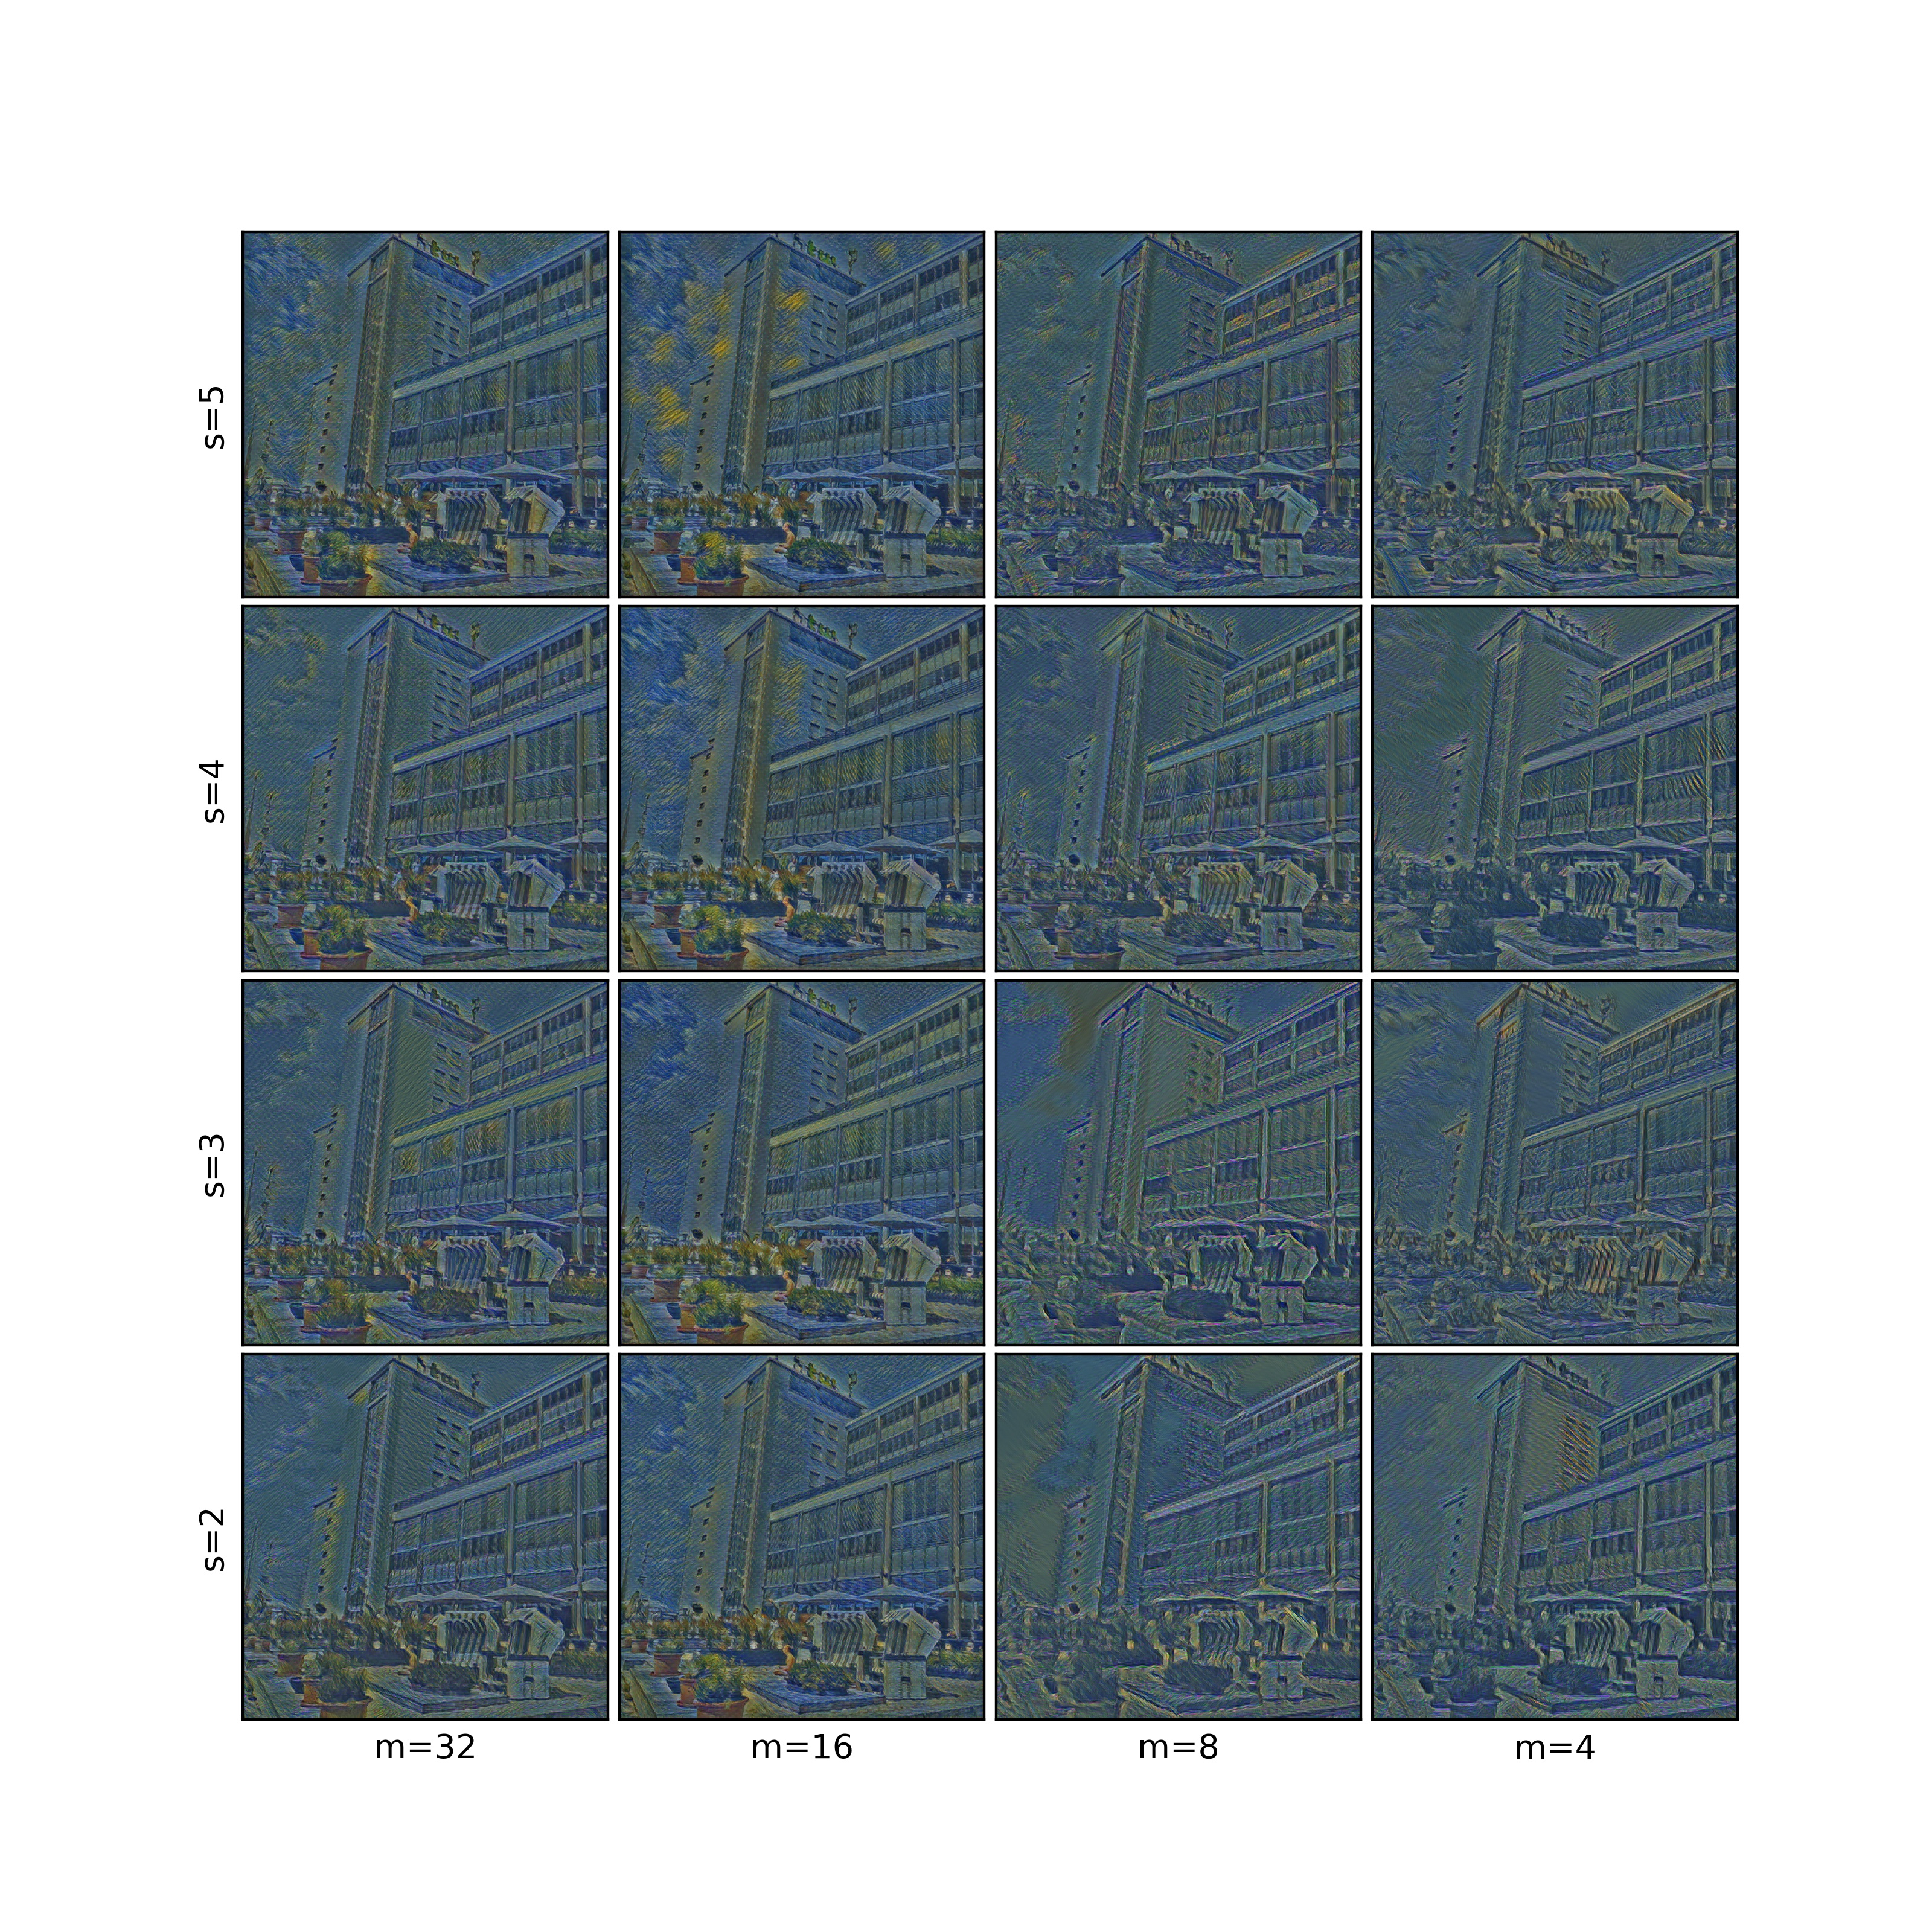
\includegraphics[width=1.00\textwidth]{resources/content/experiments/fast_image_grid_experiment1.jpg}
	\caption{Loss: The Starry Night}
	\label{img:loss_the_starry_night}
\end{figure}

\section{Loss: The Scream}
\begin{figure}[H]
	\centering
	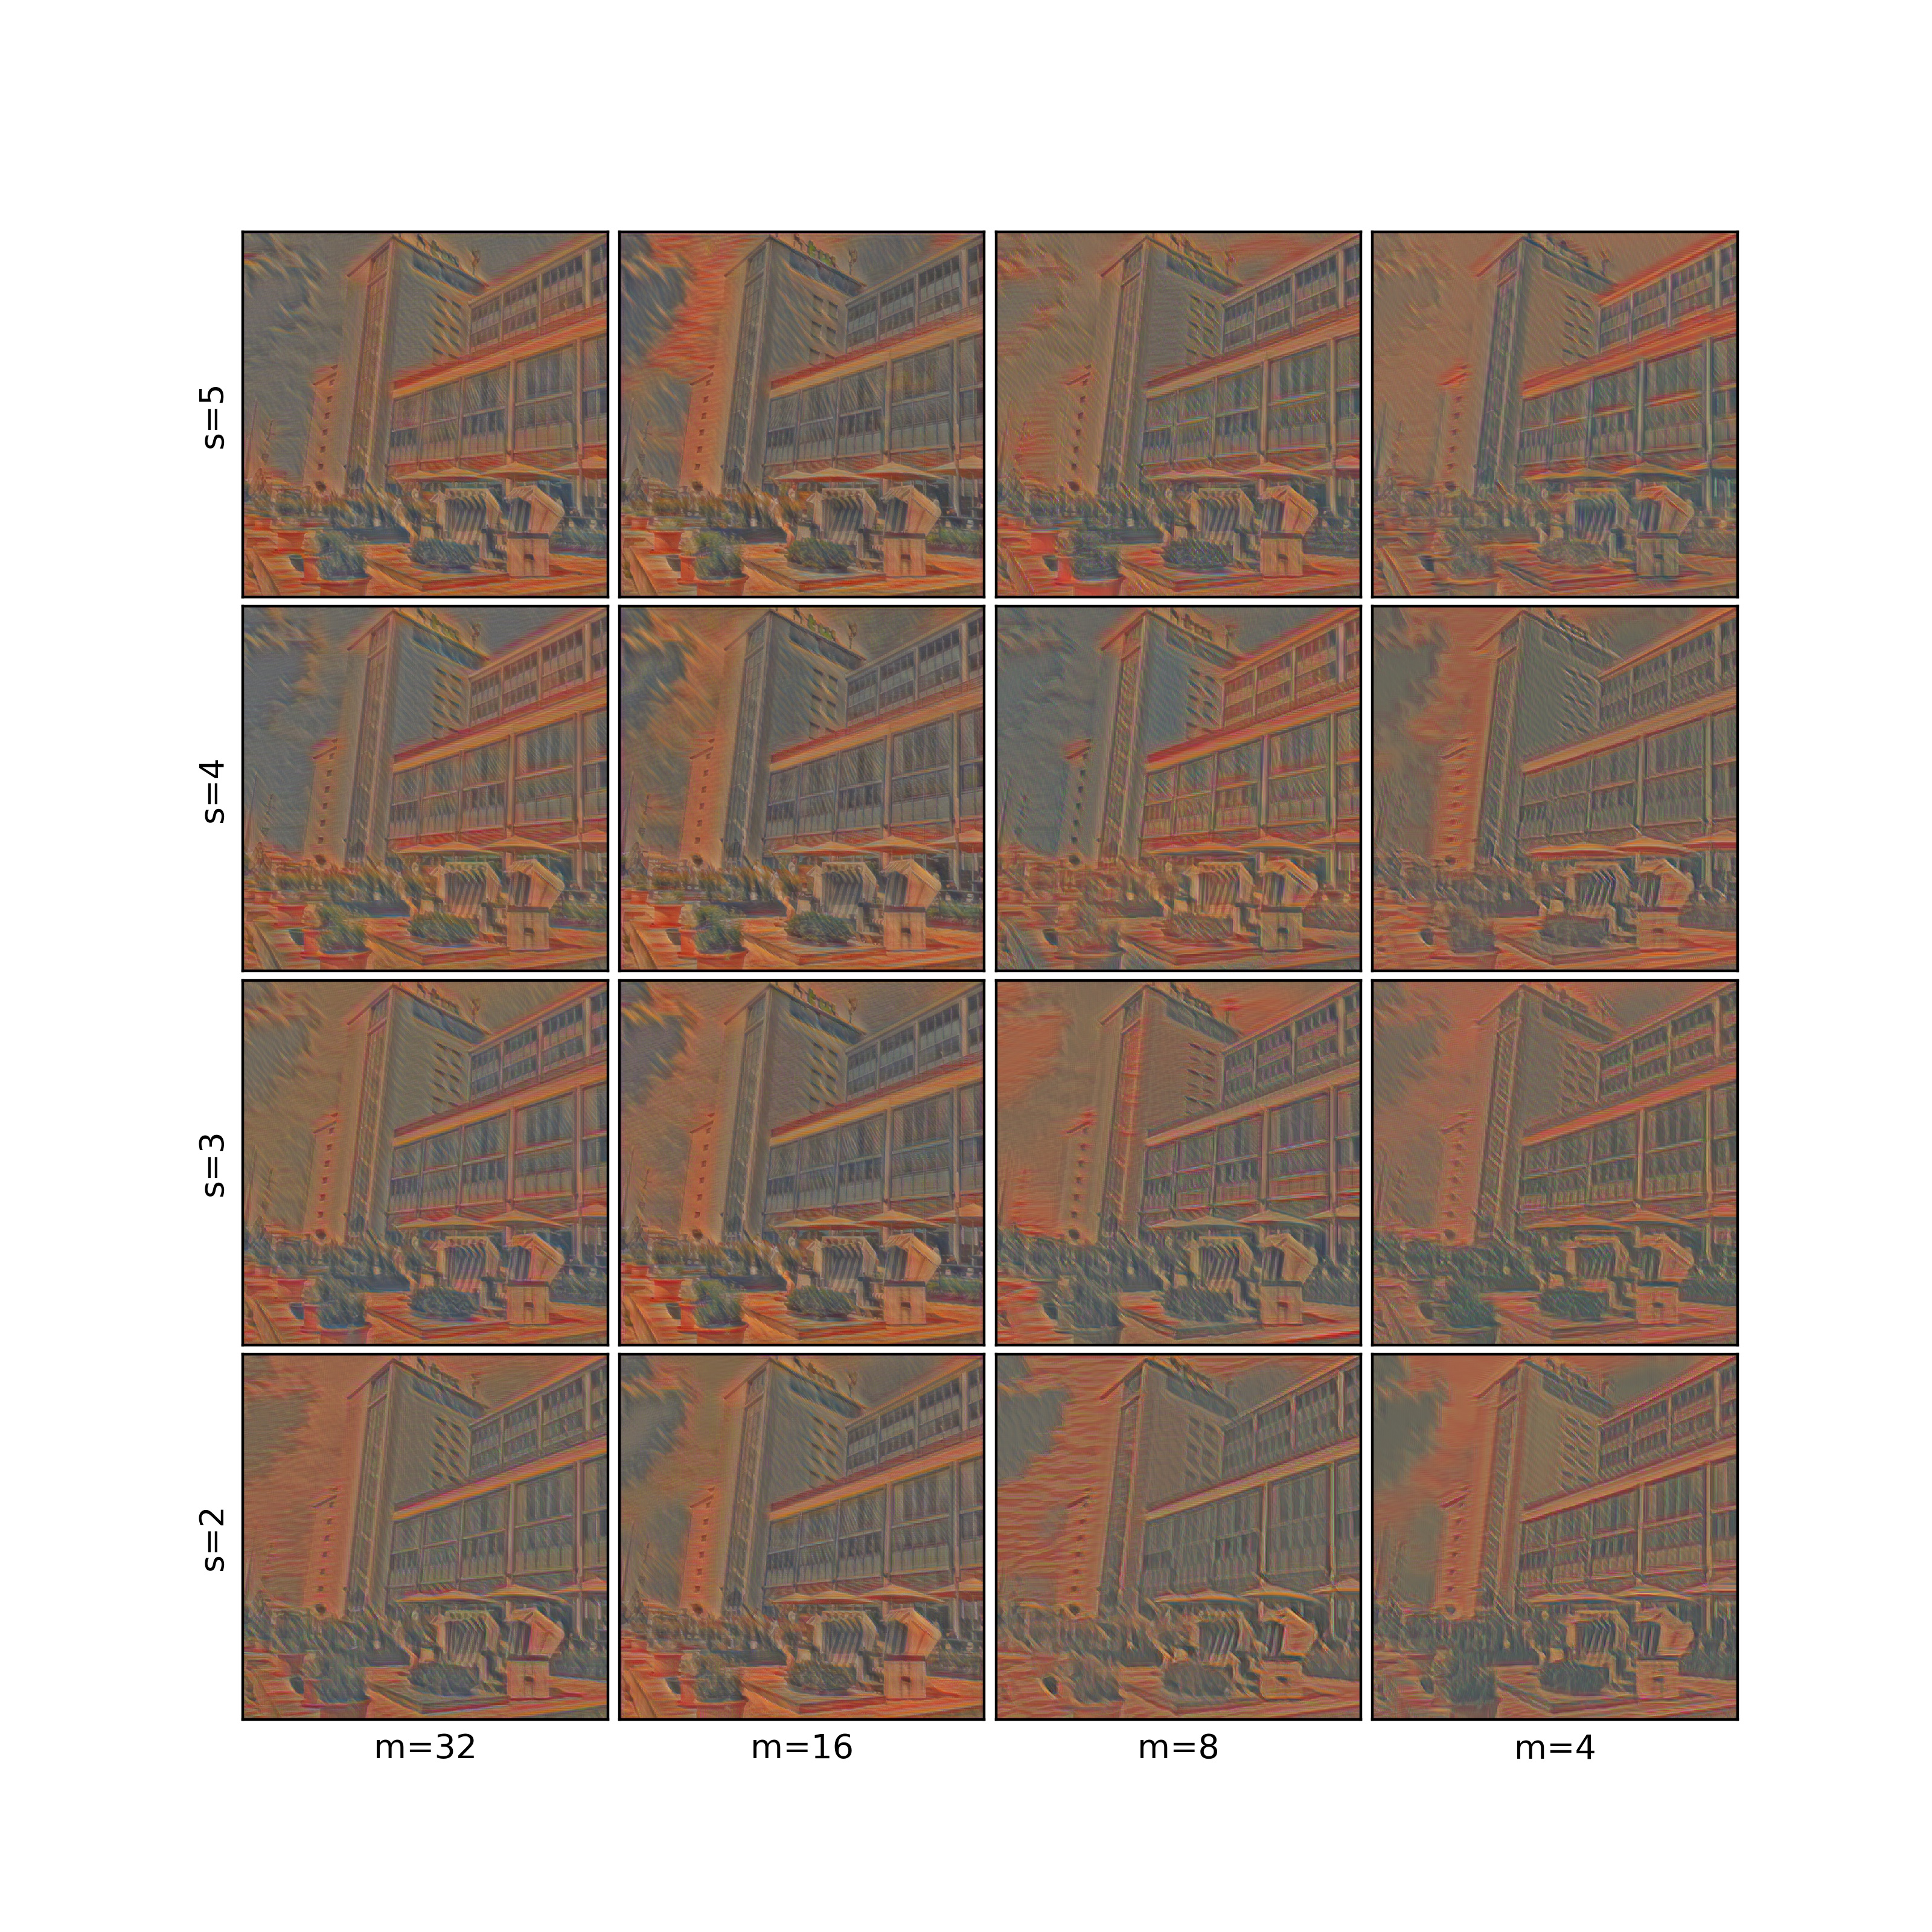
\includegraphics[width=1.00\textwidth]{resources/content/experiments/fast_image_grid_experiment2.jpg}
	\caption{Loss: The Scream}
	\label{img:loss_the_scream}
\end{figure}

\section{Ergebnisse: The Starry Night}
\begin{figure}[H]
	\centering
	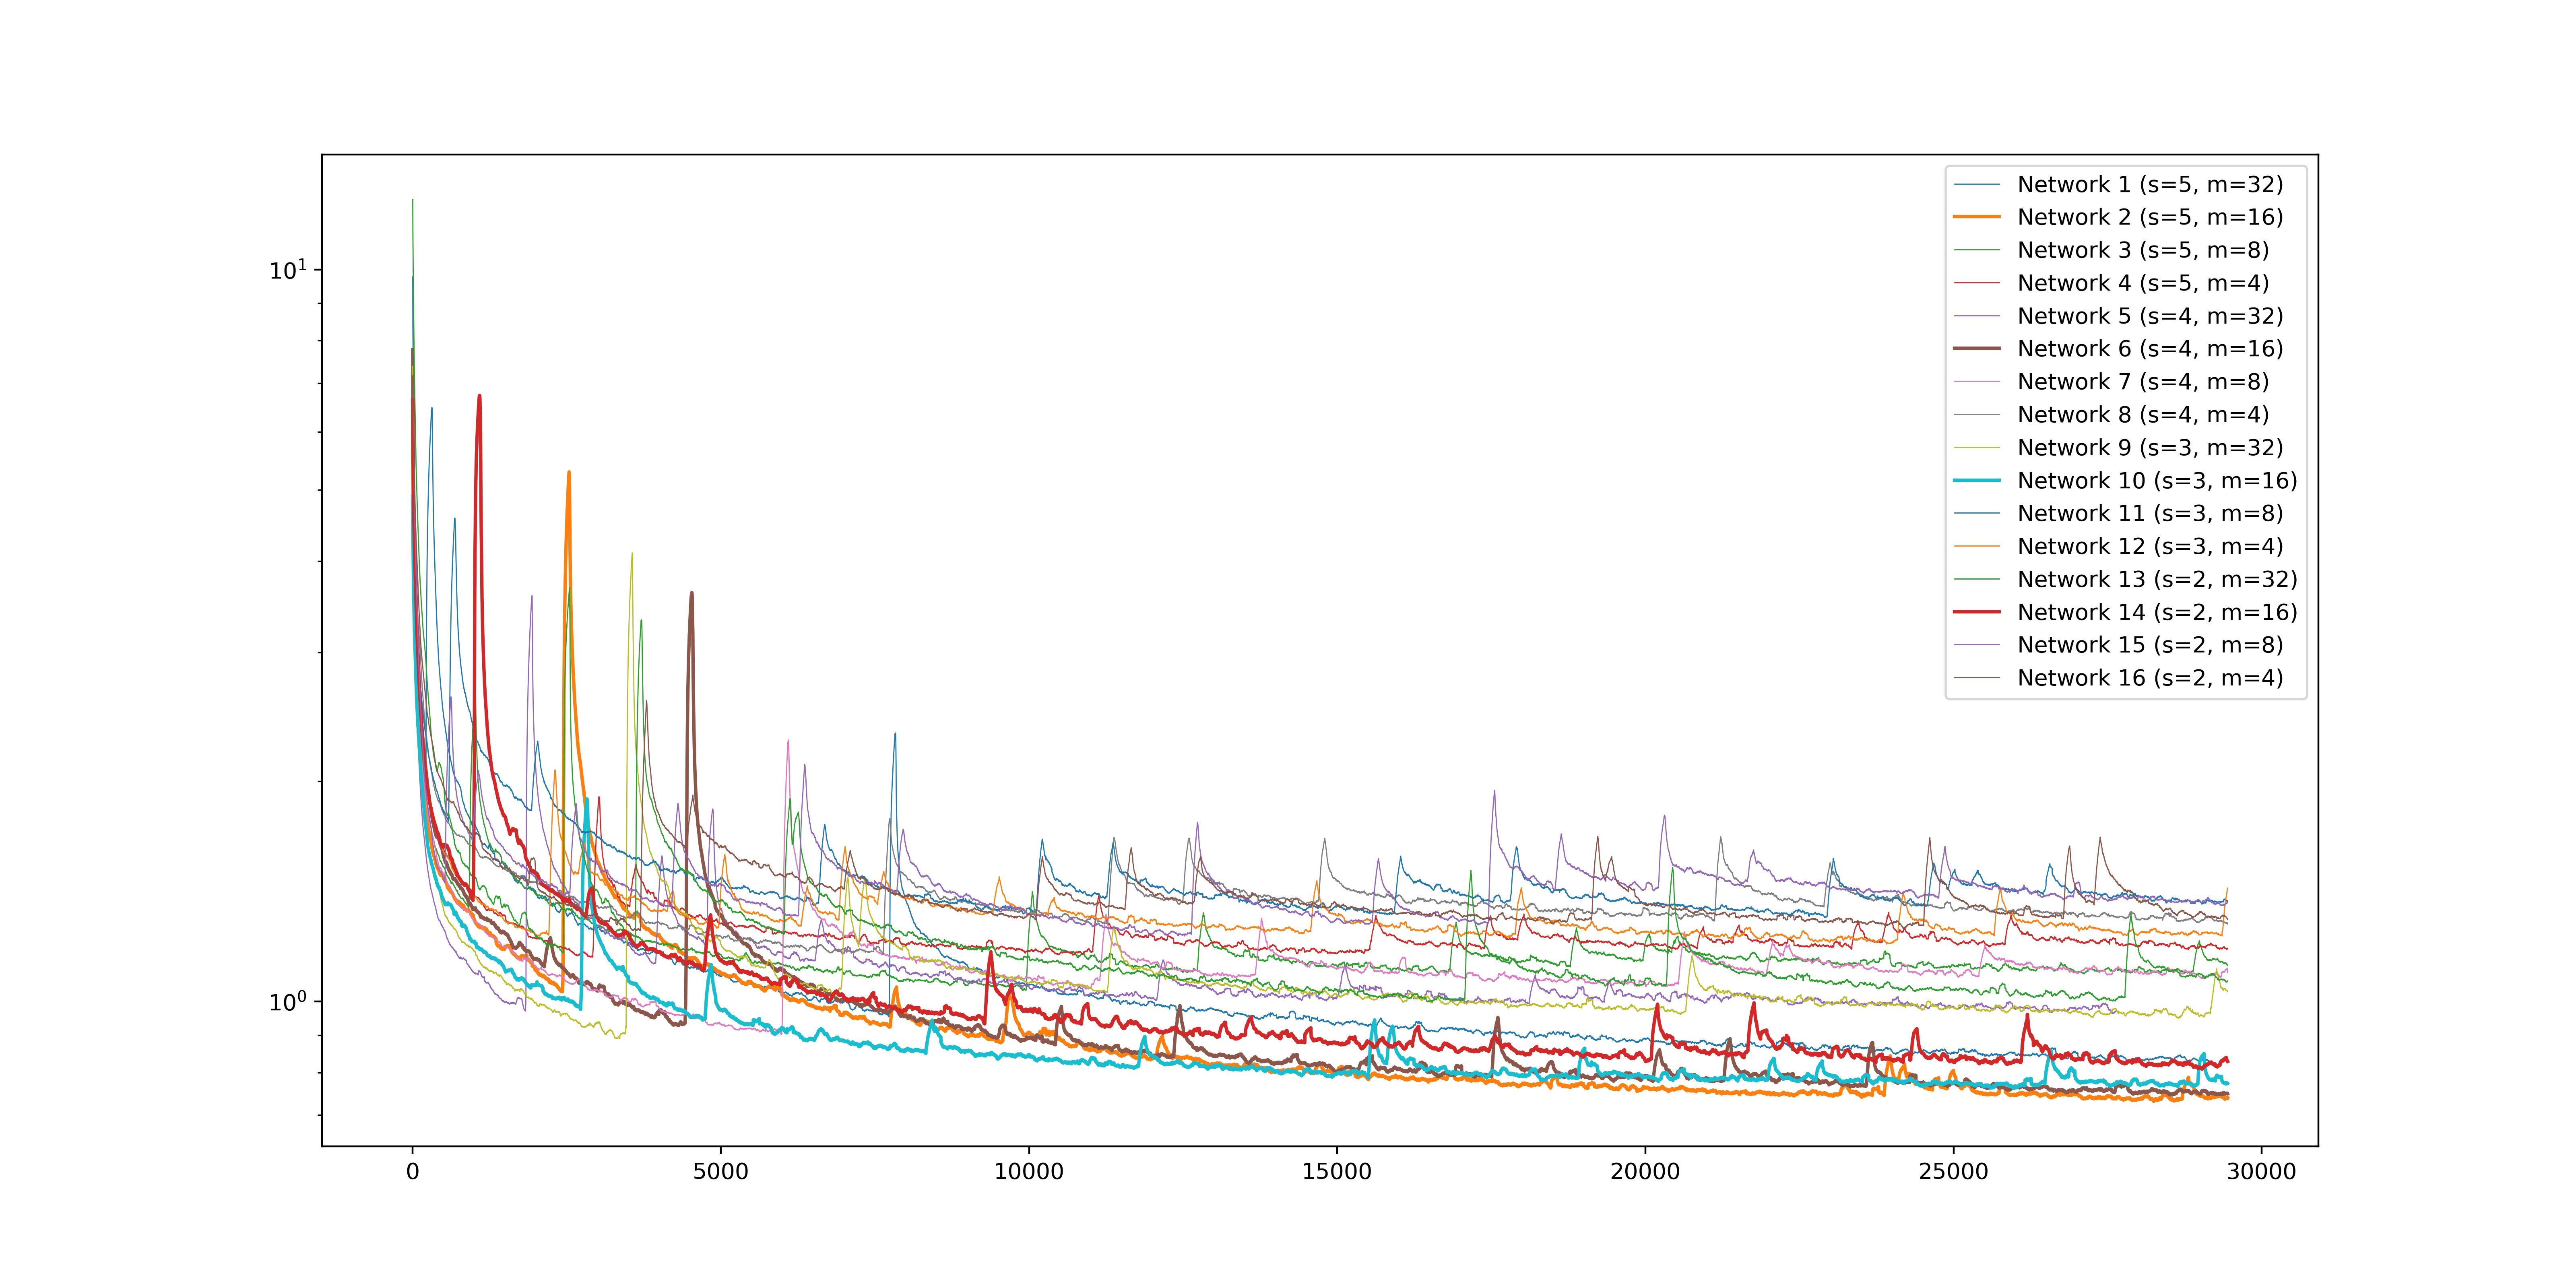
\includegraphics[width=1.00\textwidth]{resources/content/experiments/fast_loss_plot_experiment1.jpg}
	\caption{Ergebnisse: The Starry Night}
	\label{img:results_the_starry_night}
\end{figure}

\section{Ergebnisse: The Scream}
\begin{figure}[H]
	\centering
	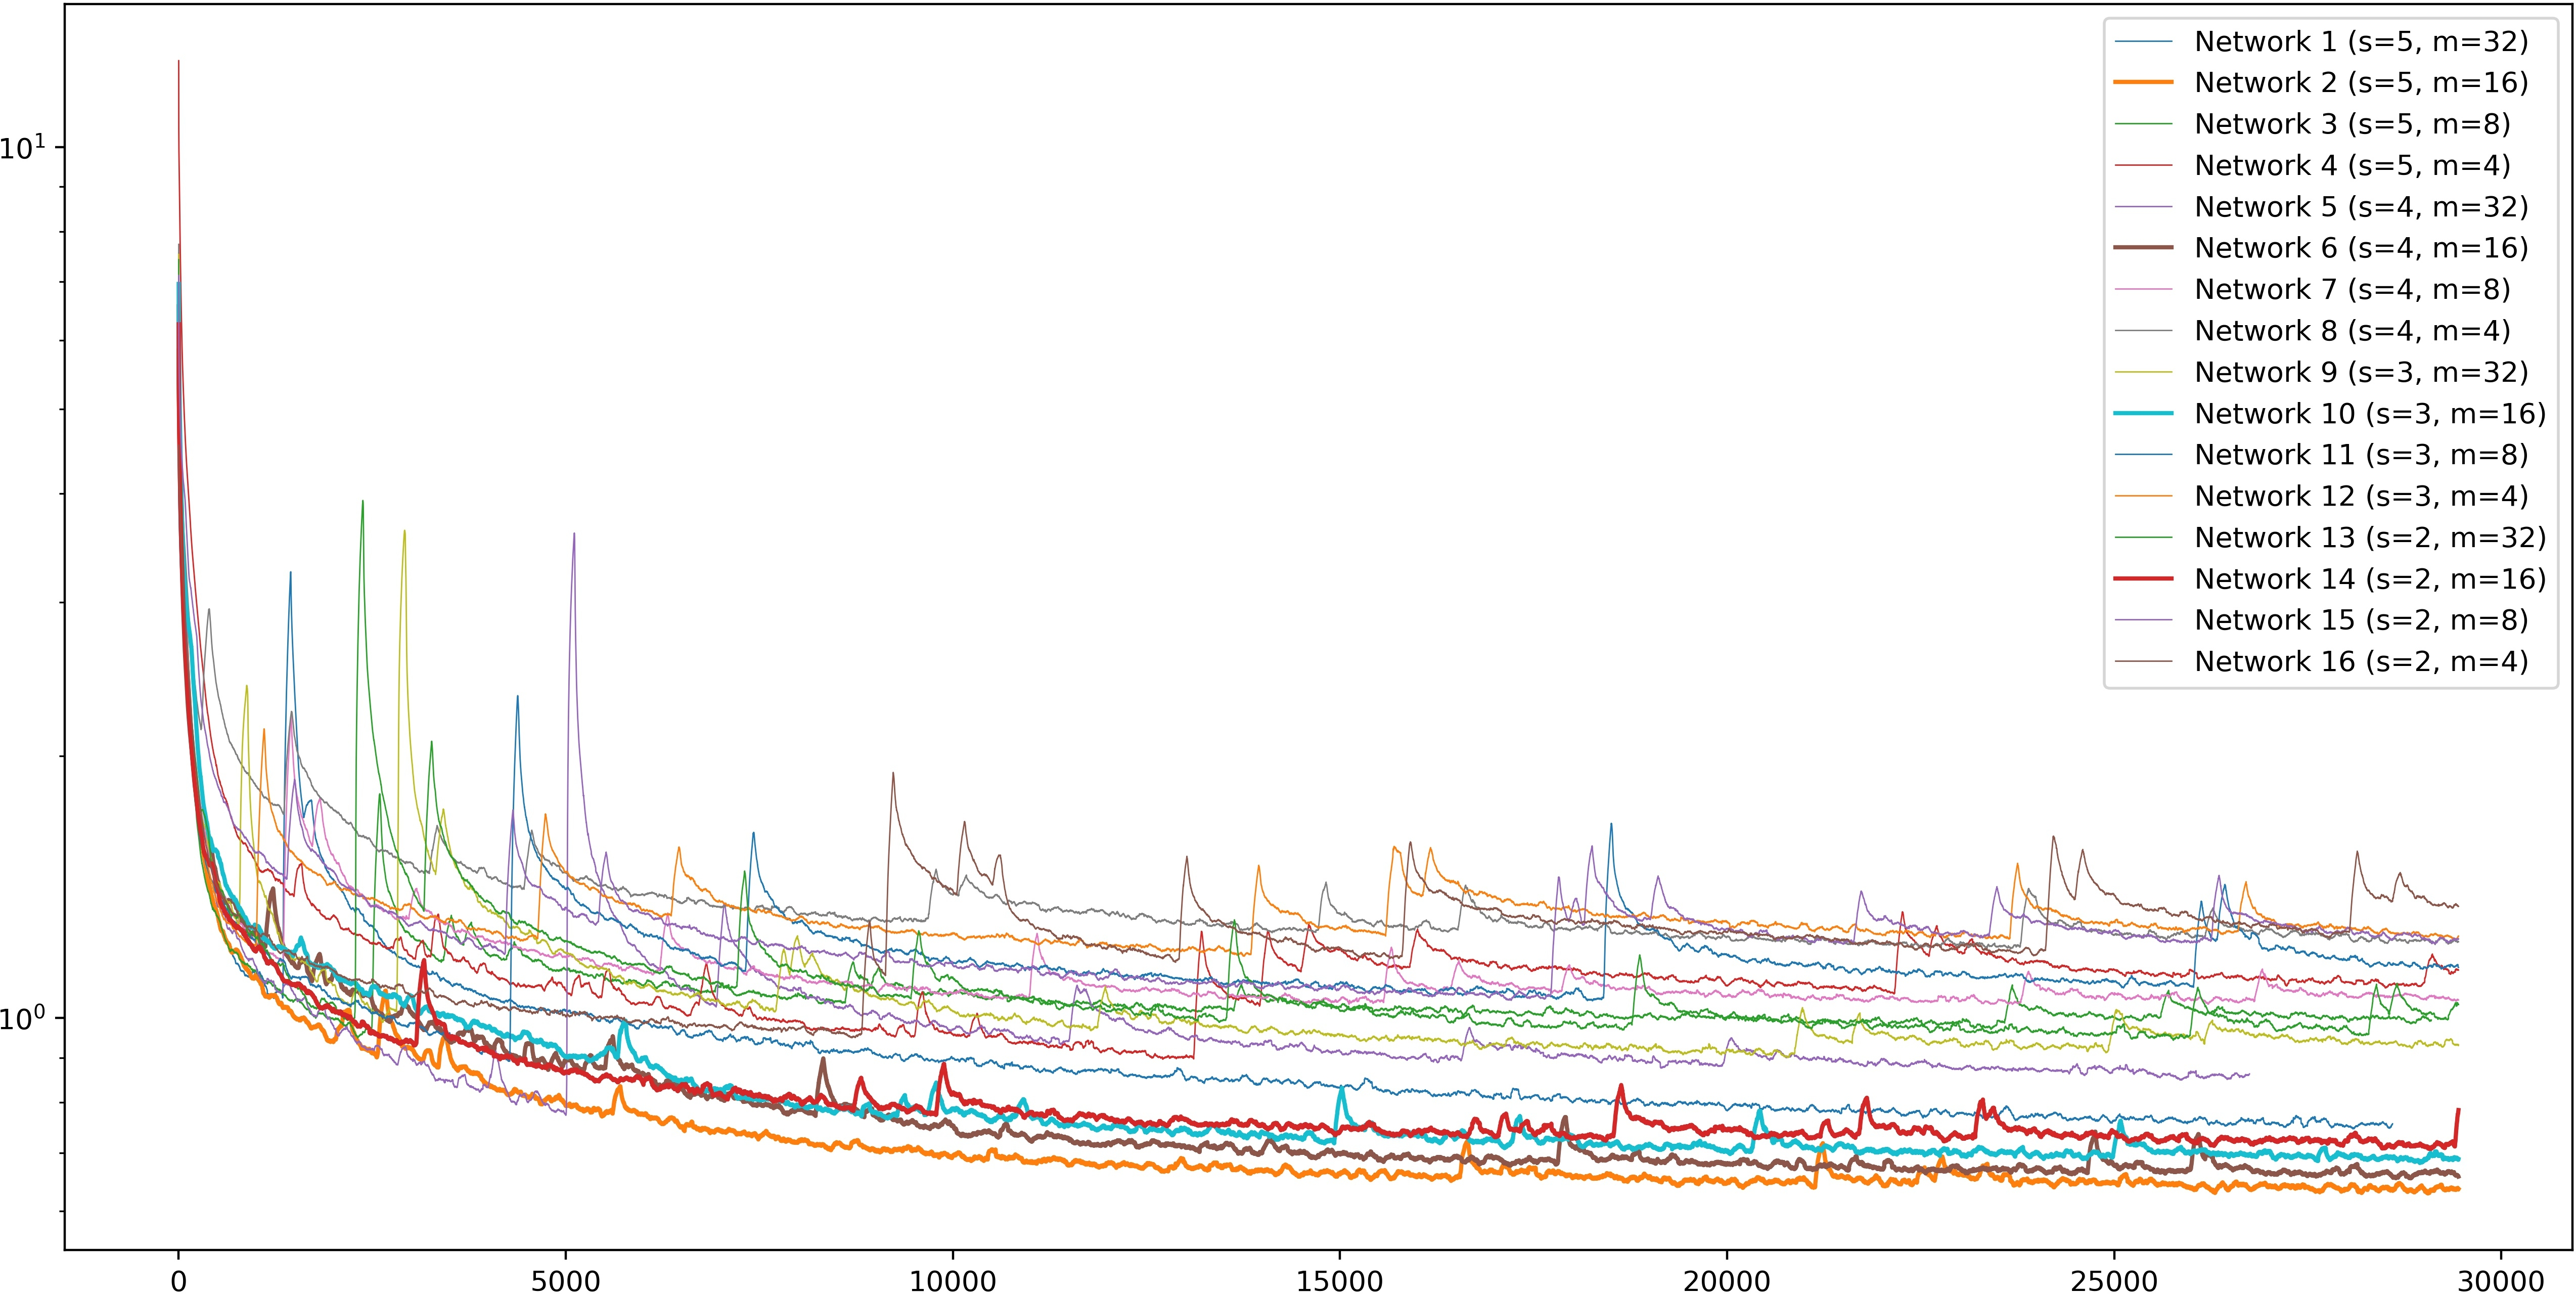
\includegraphics[width=1.00\textwidth]{resources/content/experiments/fast_loss_plot_experiment2.jpg}
	\caption{Ergebnisse: The Scream}
	\label{img:results_the_scream}
\end{figure}

\section{Trainierte Modelle}
\begin{figure}[H]
    \centering

    \begin{subfigure}[h]{0.32\textwidth}
        \centering
        \quad
    \end{subfigure}
    \begin{subfigure}[h]{0.32\textwidth}
        \centering
        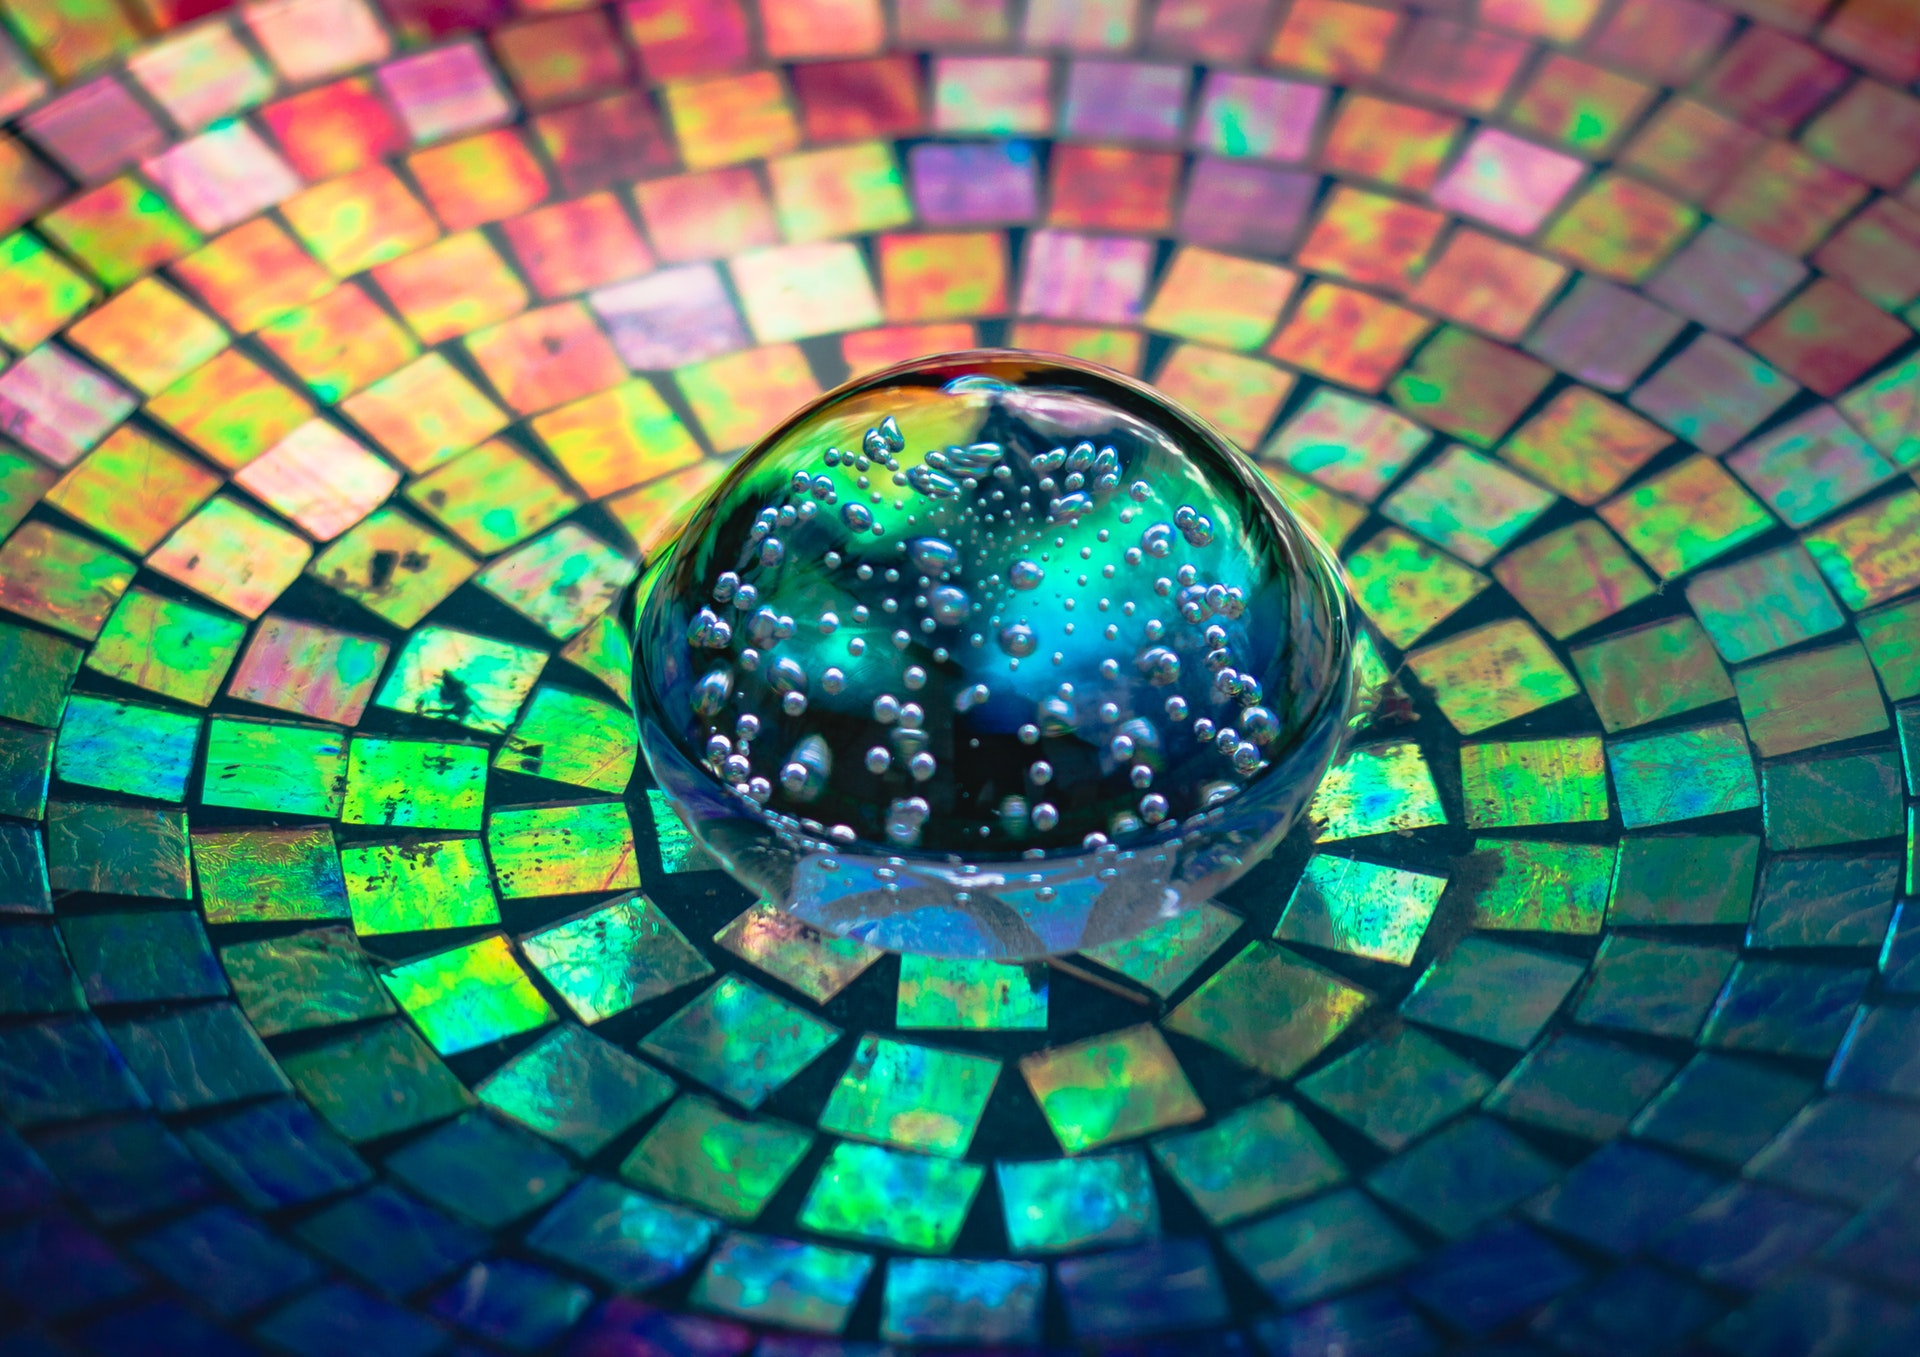
\includegraphics[width=\textwidth]{resources/content/style/crystal_glass_on_a_colorful_background.jpg}
    \end{subfigure}
    \begin{subfigure}[h]{0.32\textwidth}
        \centering
        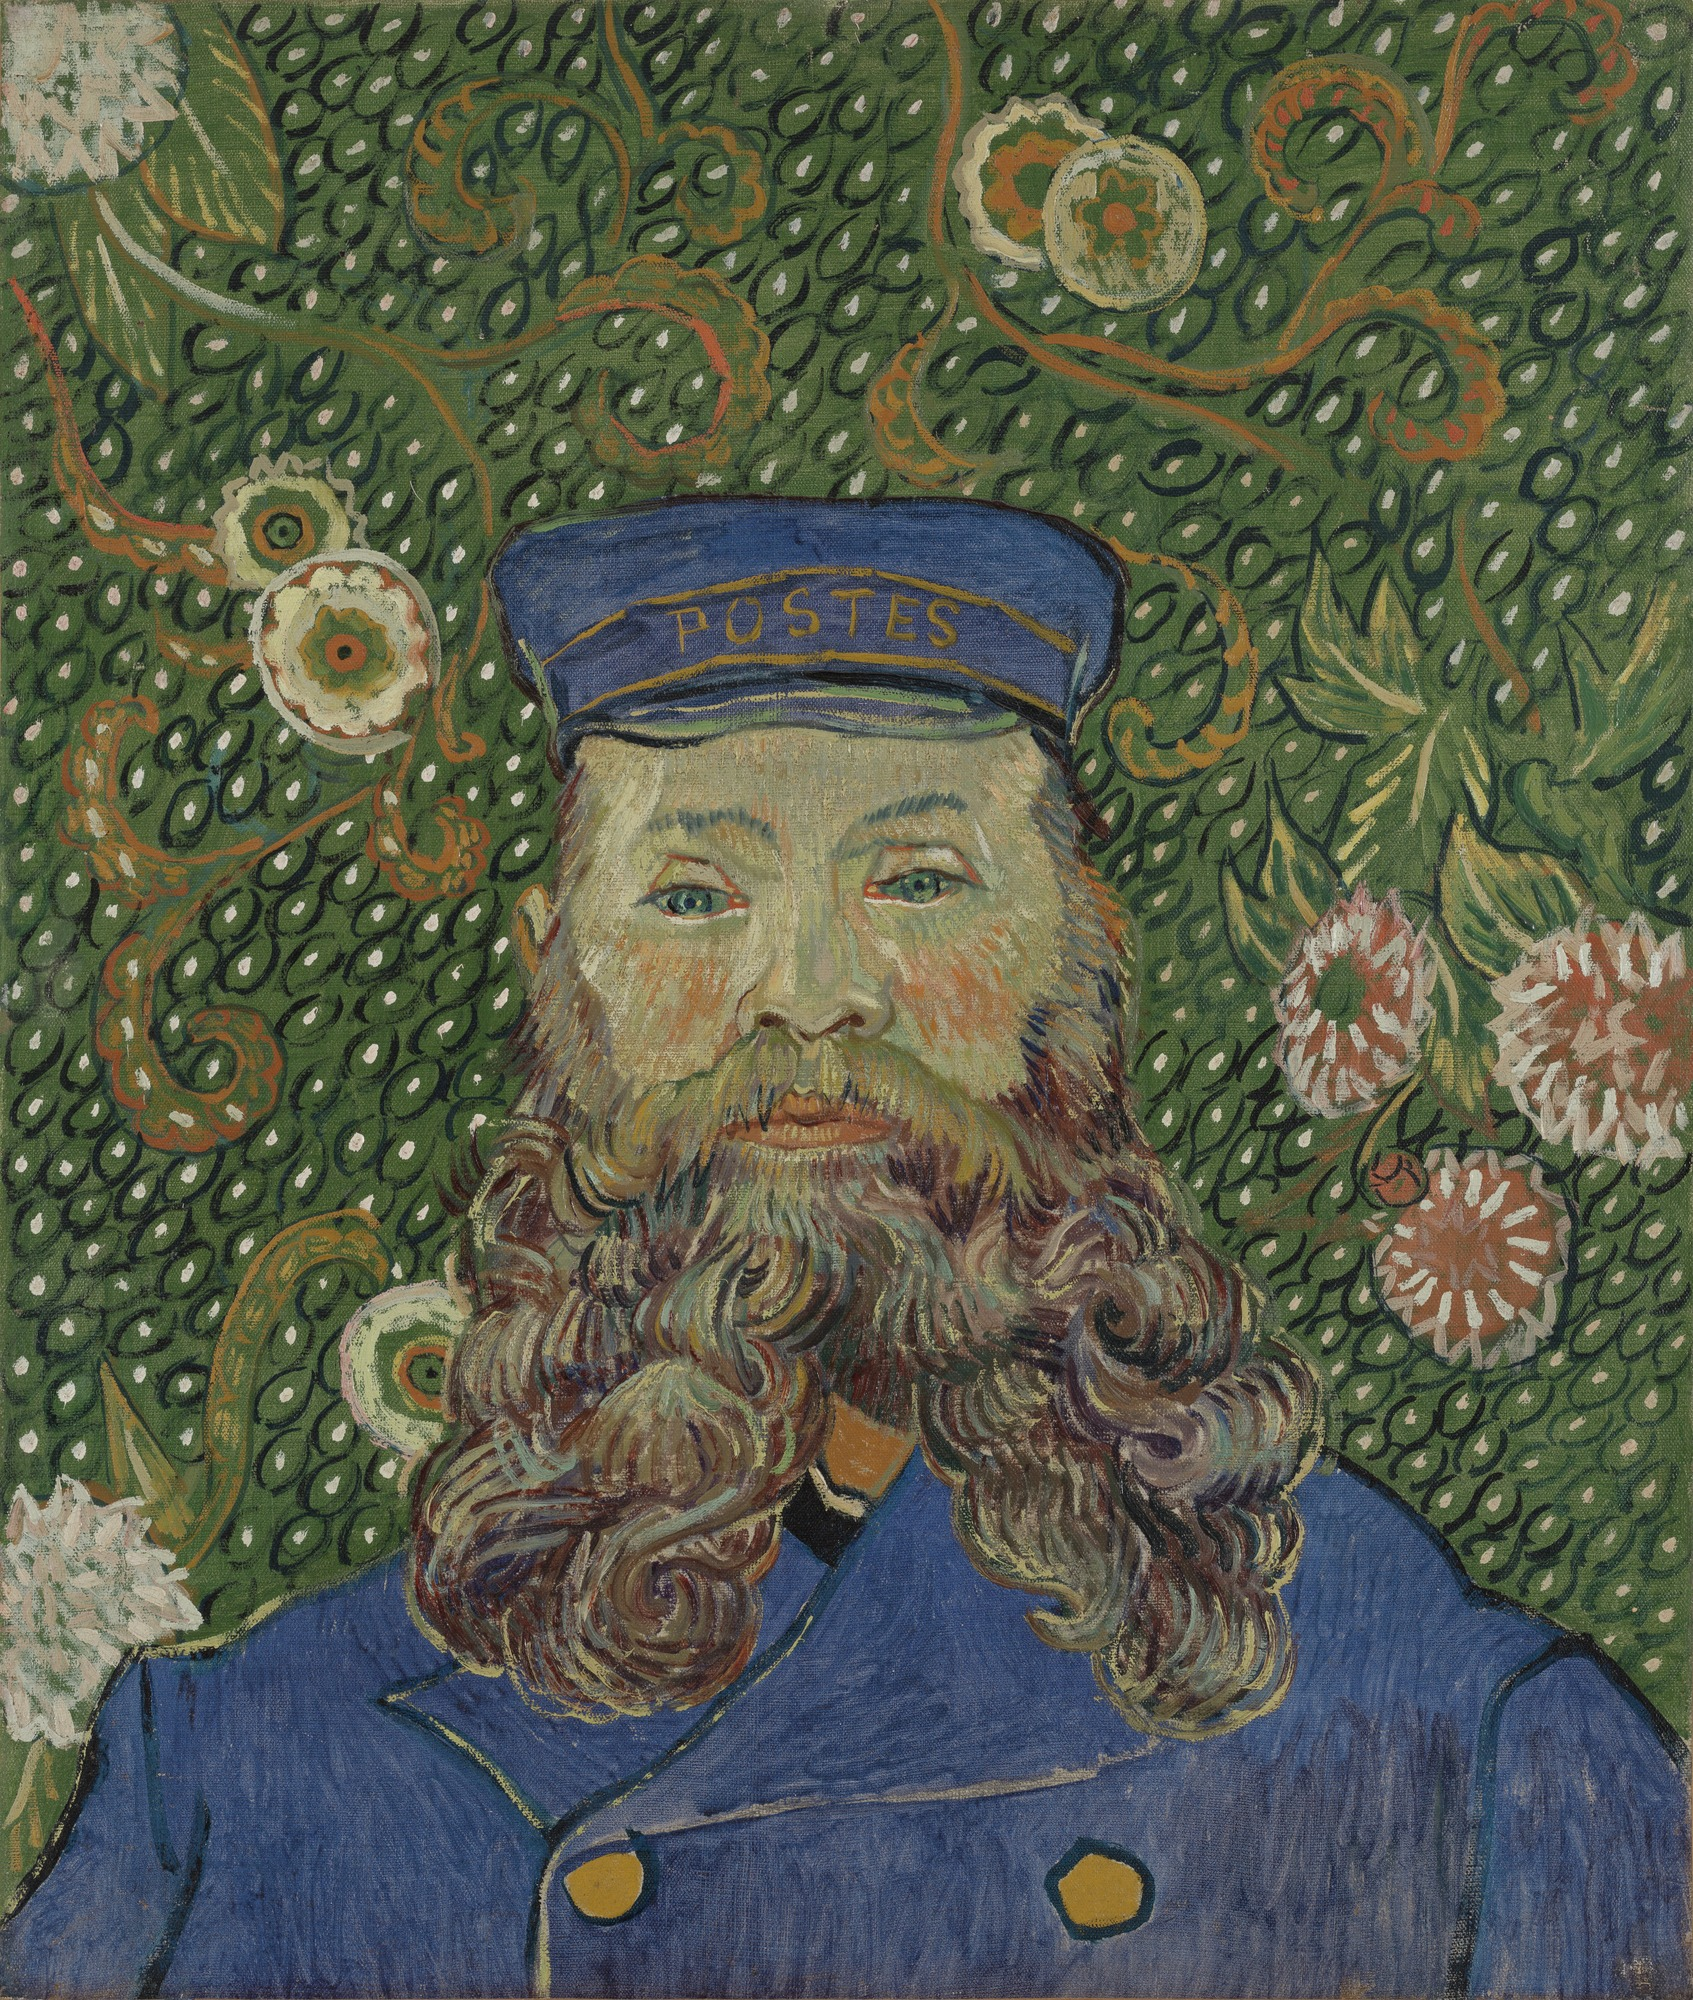
\includegraphics[width=\textwidth]{resources/content/style/portrait_of_joseph_roulin.jpg}
    \end{subfigure}


    \begin{subfigure}[h]{0.32\textwidth}
        \centering
        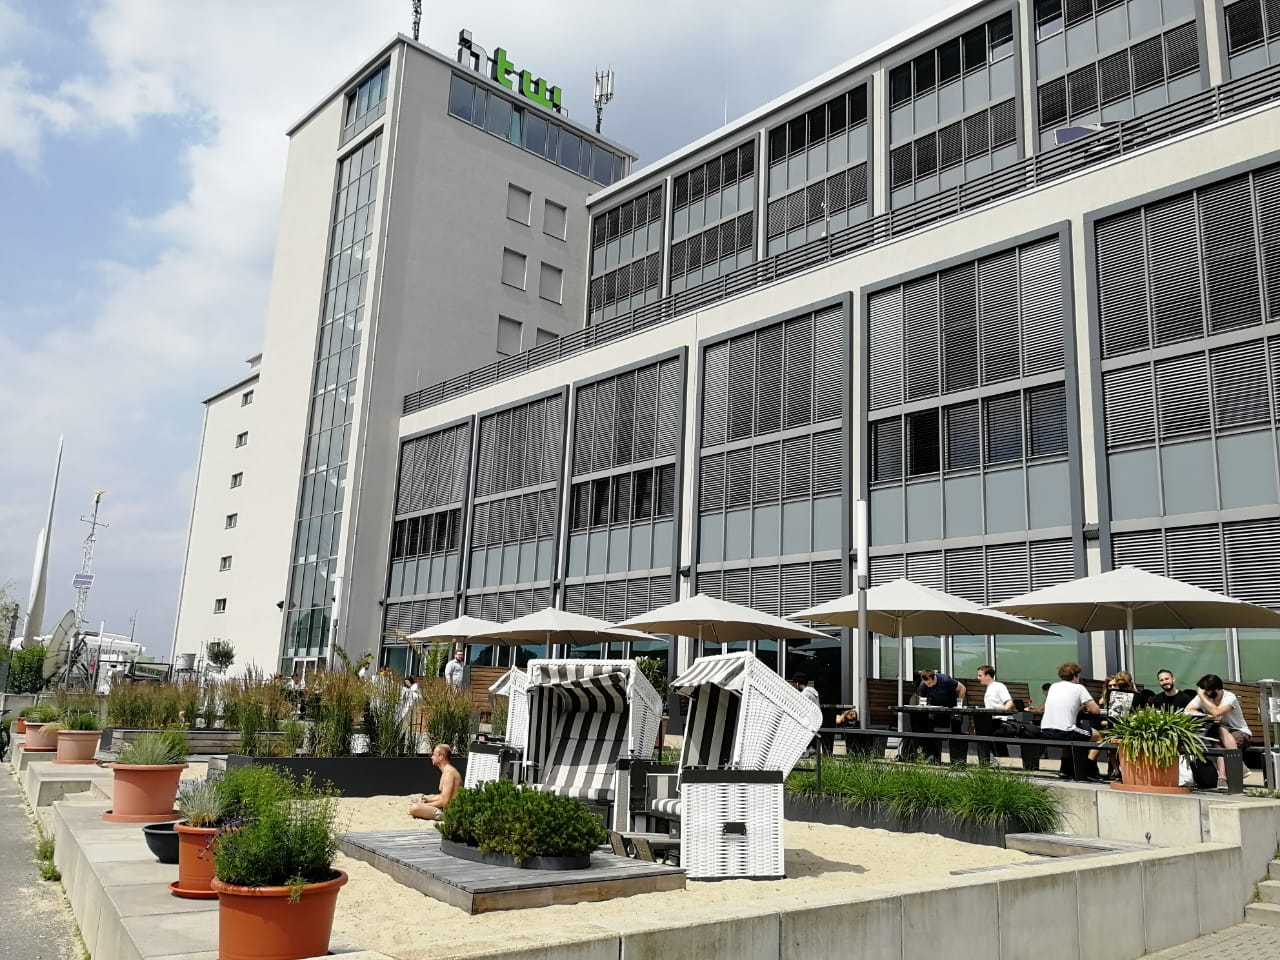
\includegraphics[width=\textwidth]{resources/content/content/htw.jpg}
    \end{subfigure}
    \begin{subfigure}[h]{0.32\textwidth}
        \centering
        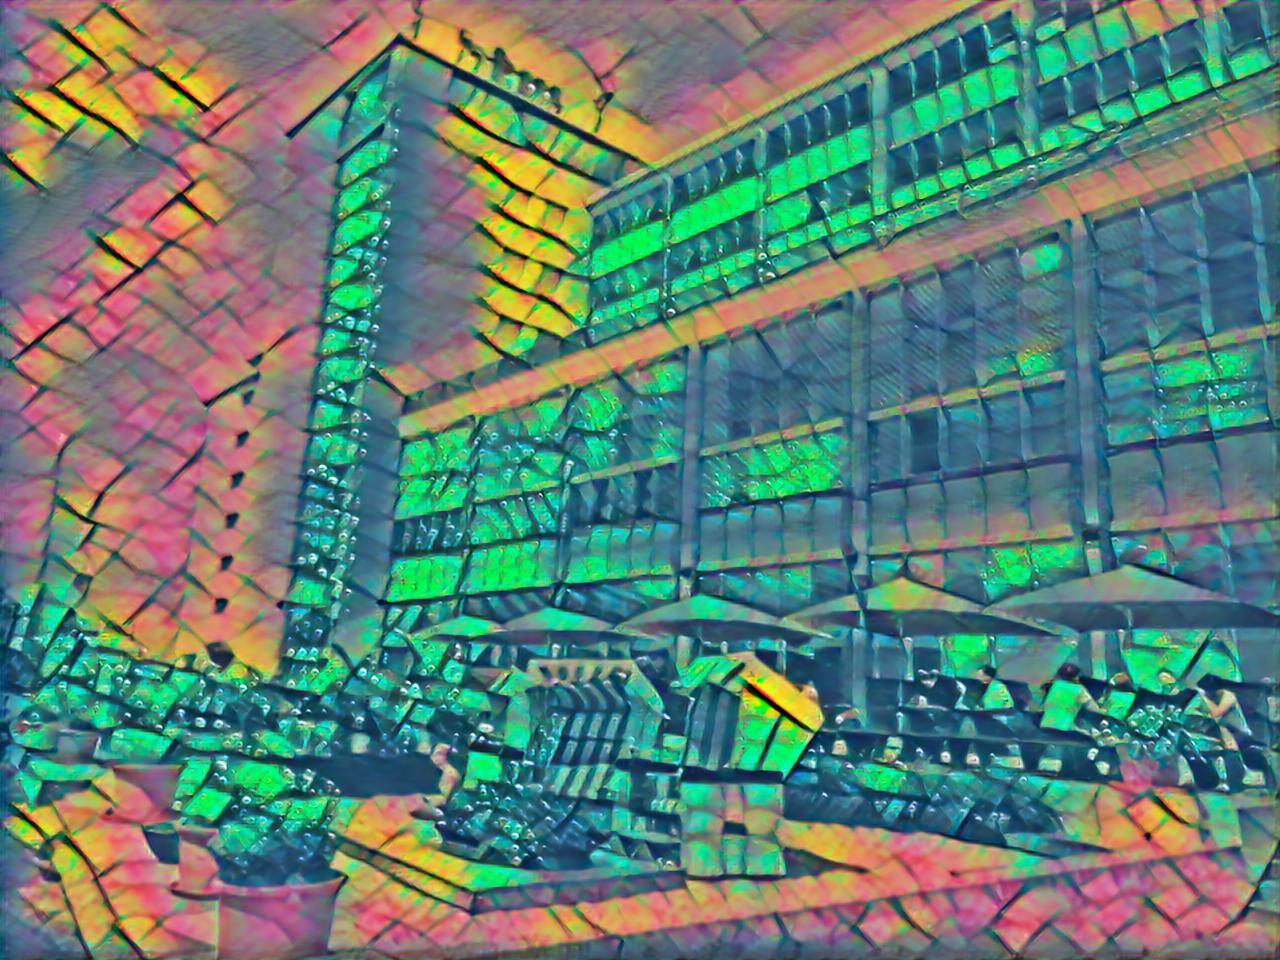
\includegraphics[width=\textwidth]{resources/content/experiments/htw-vgg16_crystal_glass_on_a_colorful_background.jpg}
    \end{subfigure}
    \begin{subfigure}[h]{0.32\textwidth}
        \centering
        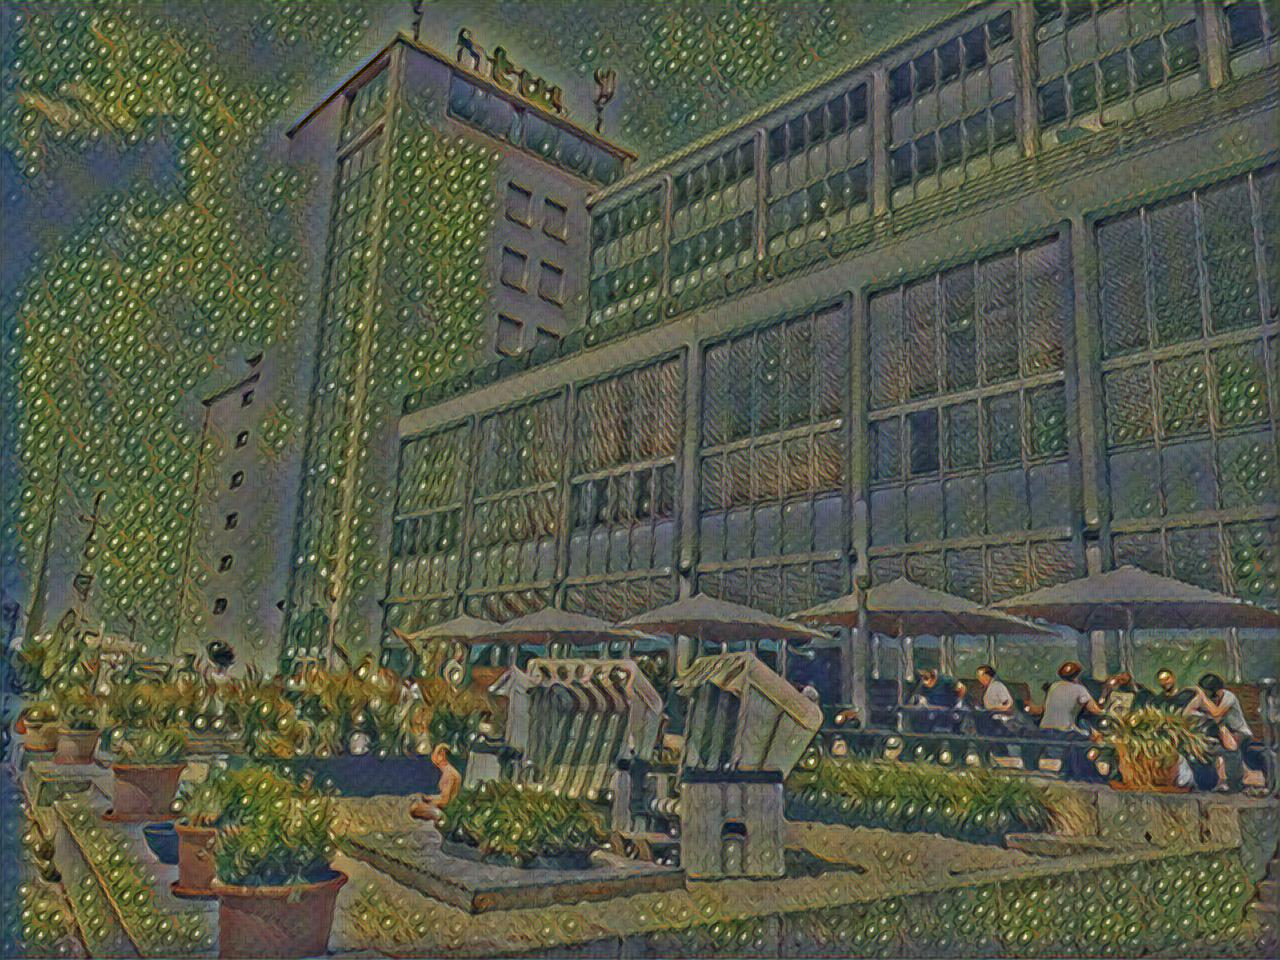
\includegraphics[width=\textwidth]{resources/content/experiments/htw-vgg16_portrait_of_joseph_roulin.jpg}
    \end{subfigure}


    \begin{subfigure}[h]{0.32\textwidth}
        \centering
        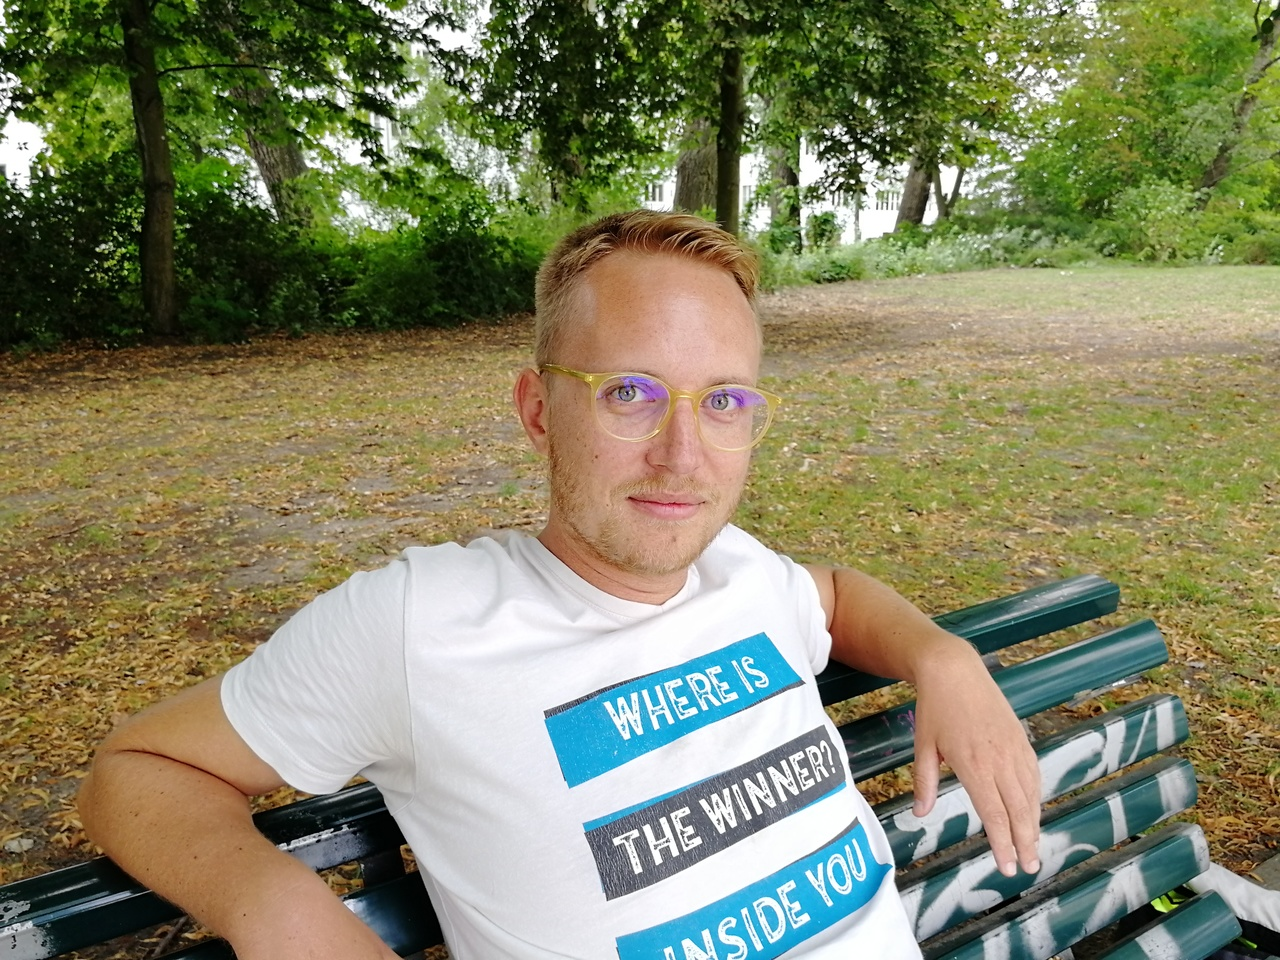
\includegraphics[width=\textwidth]{resources/content/content/ich.jpg}
    \end{subfigure}
    \begin{subfigure}[h]{0.32\textwidth}
        \centering
        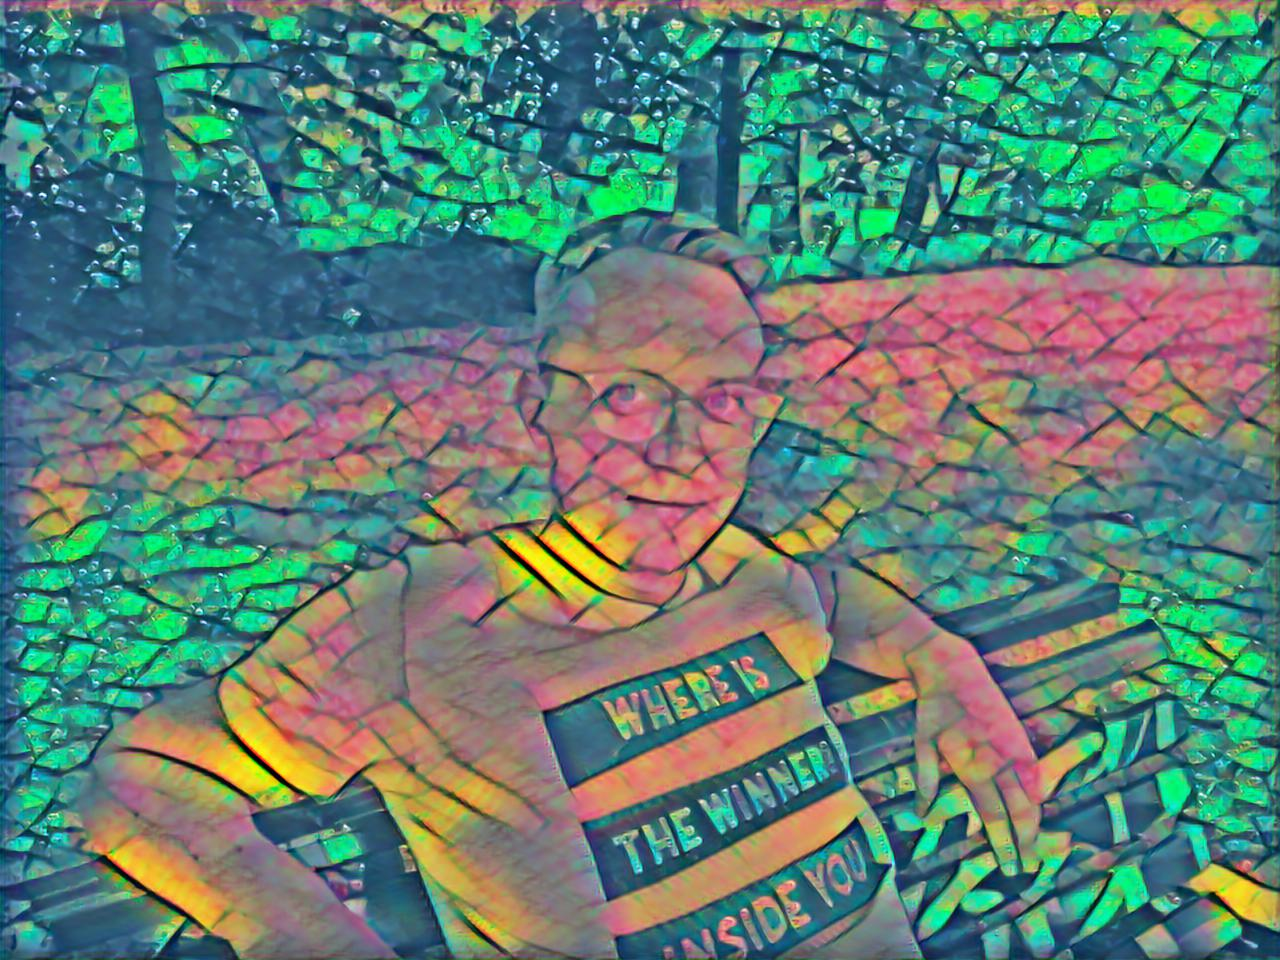
\includegraphics[width=\textwidth]{resources/content/experiments/ich-vgg16_crystal_glass_on_a_colorful_background.jpg}
    \end{subfigure}
    \begin{subfigure}[h]{0.32\textwidth}
        \centering
        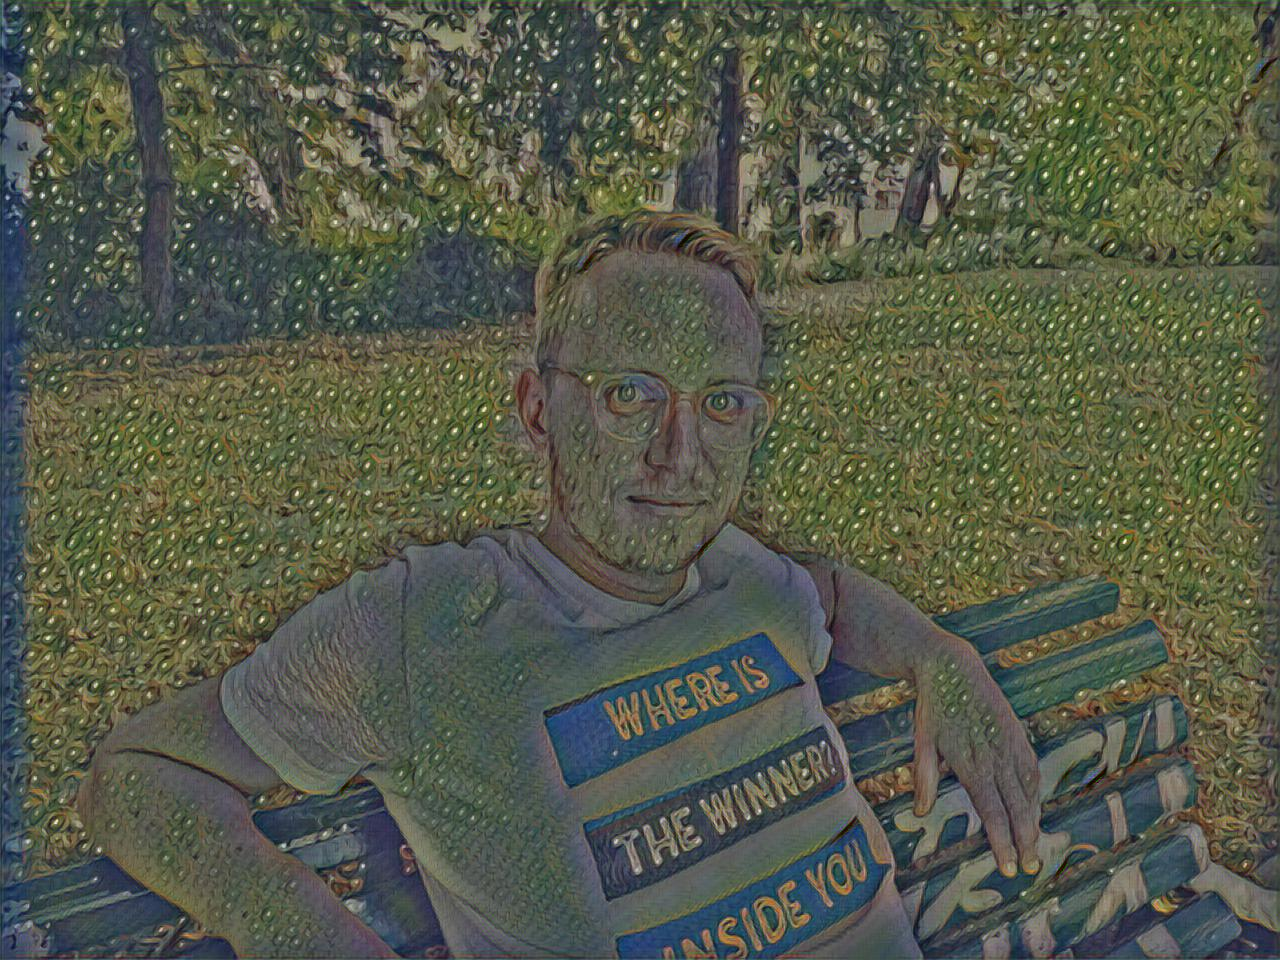
\includegraphics[width=\textwidth]{resources/content/experiments/ich-vgg16_portrait_of_joseph_roulin.jpg}
    \end{subfigure}


    \begin{subfigure}[h]{0.32\textwidth}
        \centering
        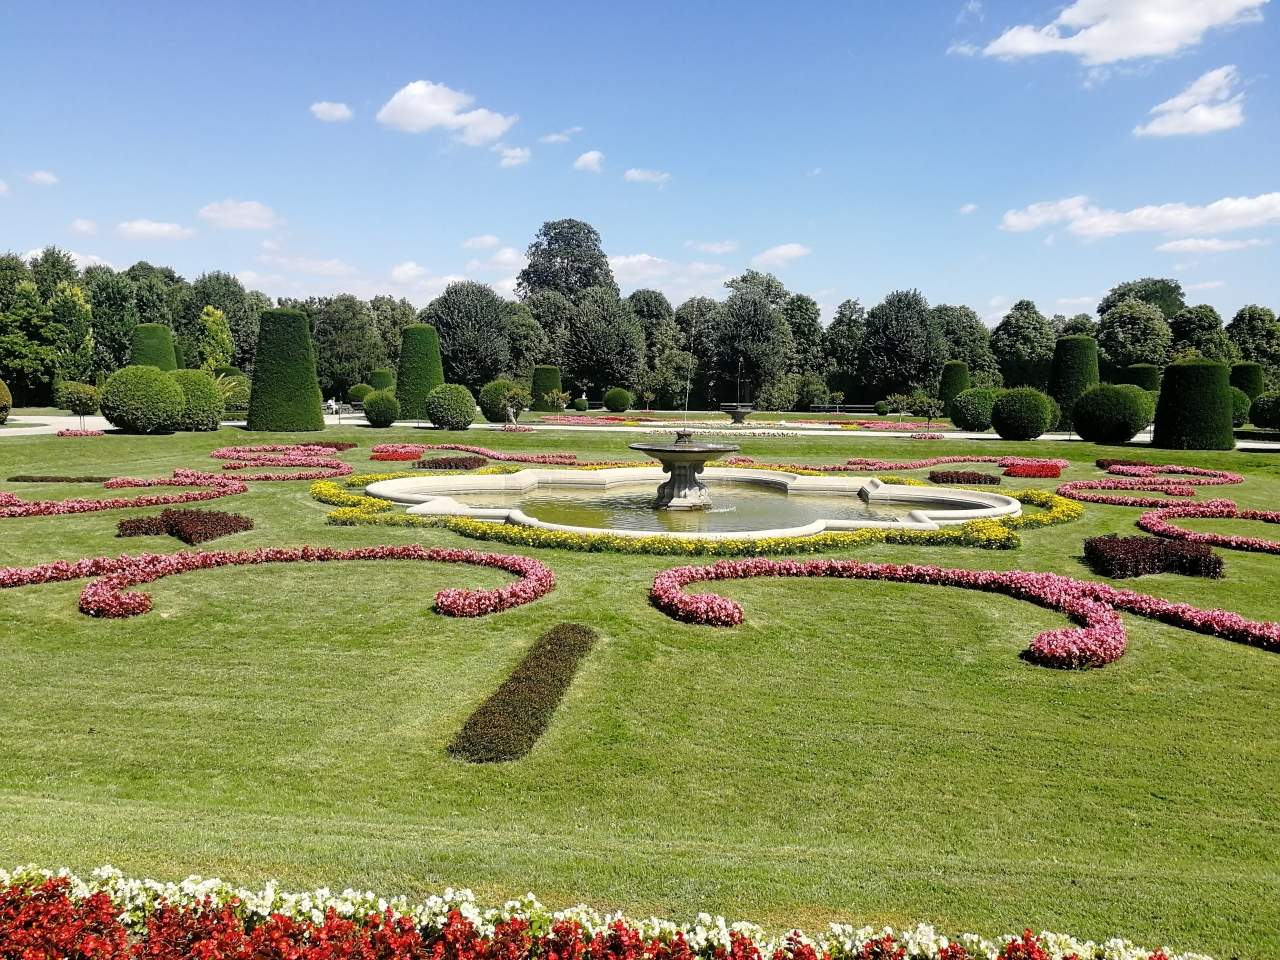
\includegraphics[width=\textwidth]{resources/content/content/garden.jpg}
    \end{subfigure}
    \begin{subfigure}[h]{0.32\textwidth}
        \centering
        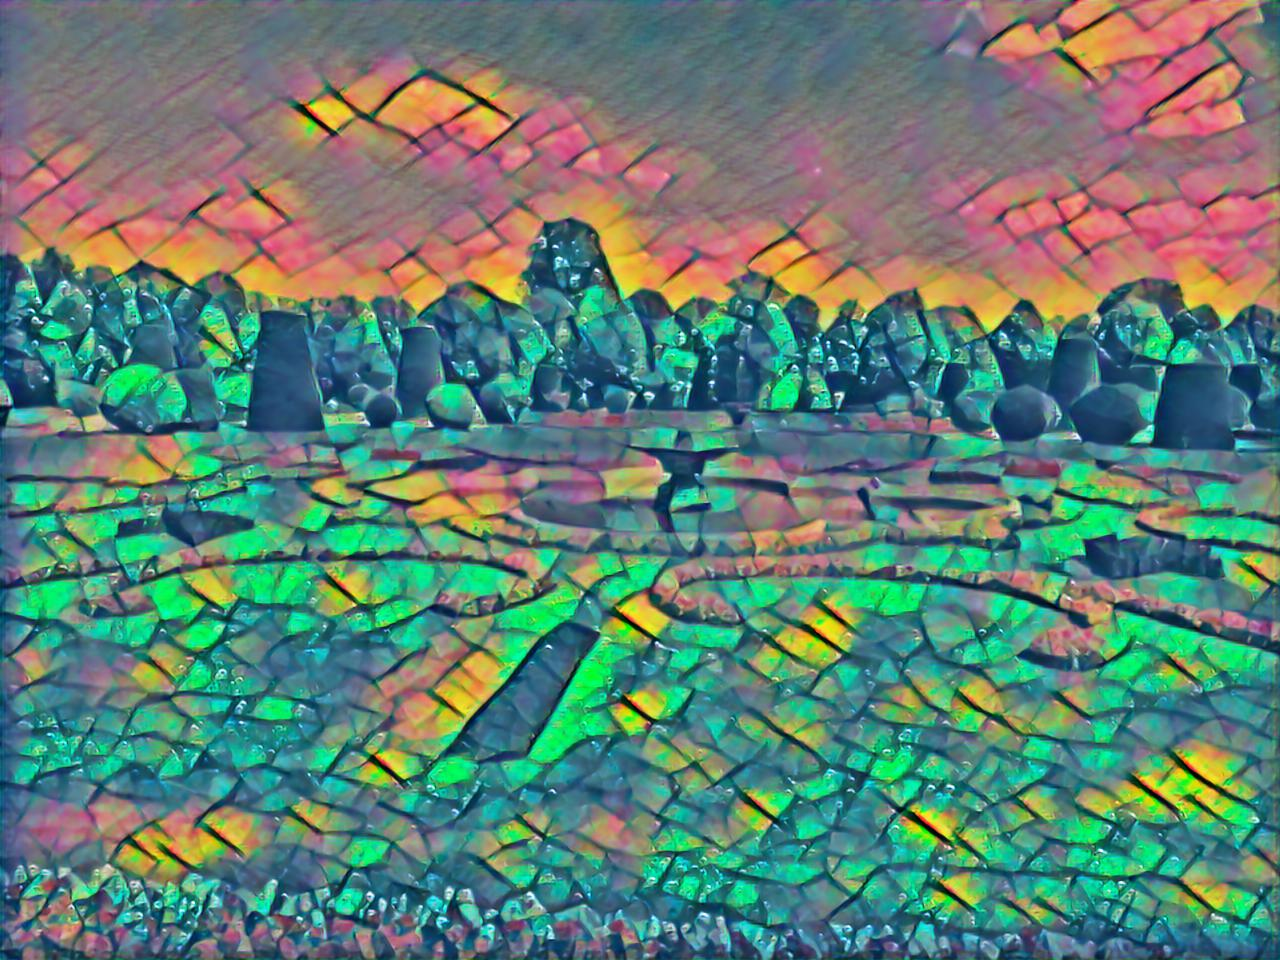
\includegraphics[width=\textwidth]{resources/content/experiments/garden-vgg16_crystal_glass_on_a_colorful_background.jpg}
    \end{subfigure}
    \begin{subfigure}[h]{0.32\textwidth}
        \centering
        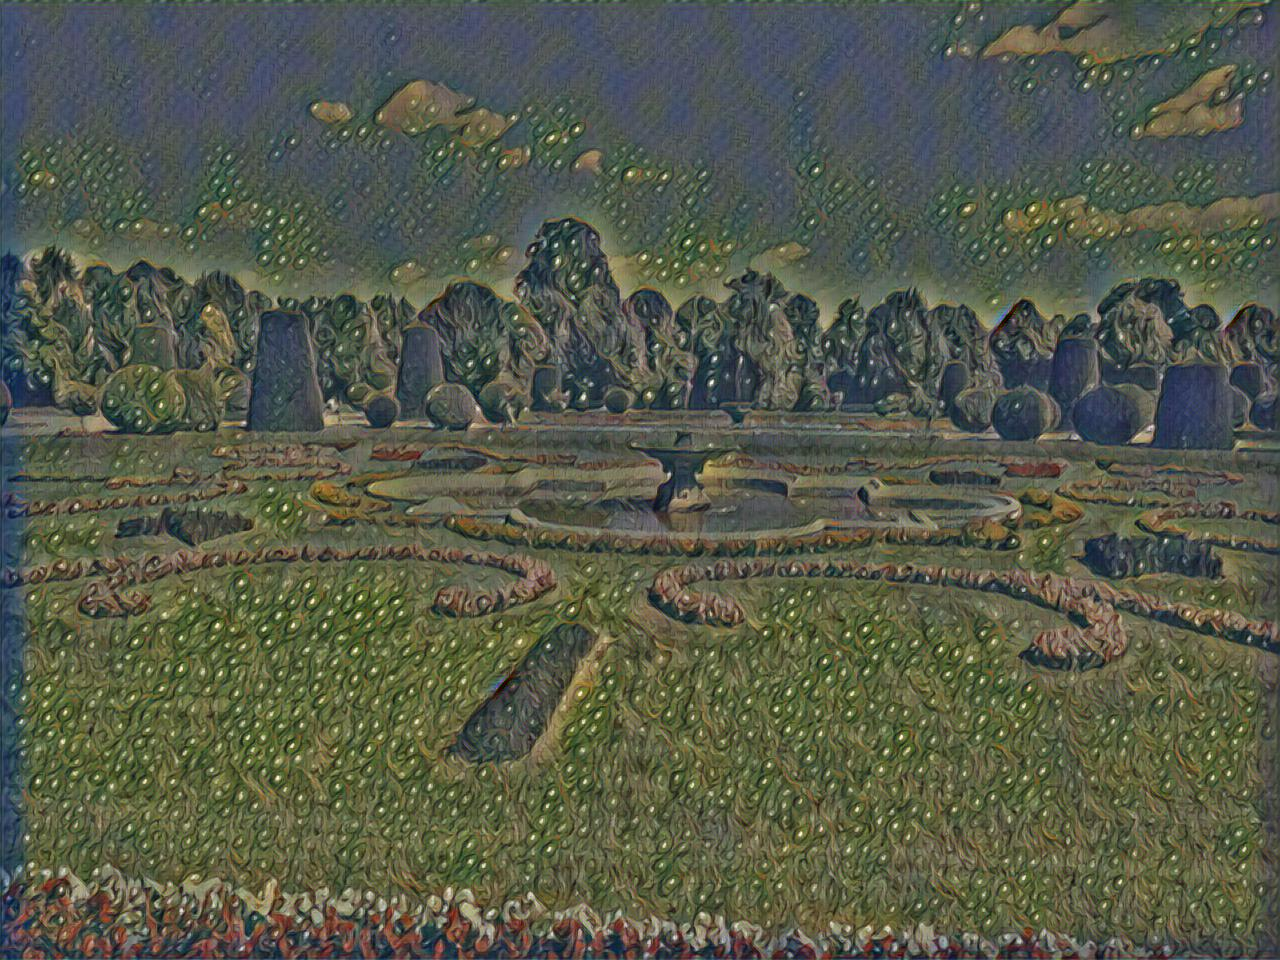
\includegraphics[width=\textwidth]{resources/content/experiments/garden-vgg16_portrait_of_joseph_roulin.jpg}
    \end{subfigure}

    \caption{Eigene Abbildungen kombiniert mit verschiedenen Stilen: \cite{crystal_glass_on_a_colorful_background_img}, \cite{portrait_of_joseph_roulin_img}}
    \label{img:trained_models1}
\end{figure}

\begin{figure}[H]
    \centering

    \begin{subfigure}[h]{0.32\textwidth}
        \centering
        \quad
    \end{subfigure}
    \begin{subfigure}[h]{0.32\textwidth}
        \centering
        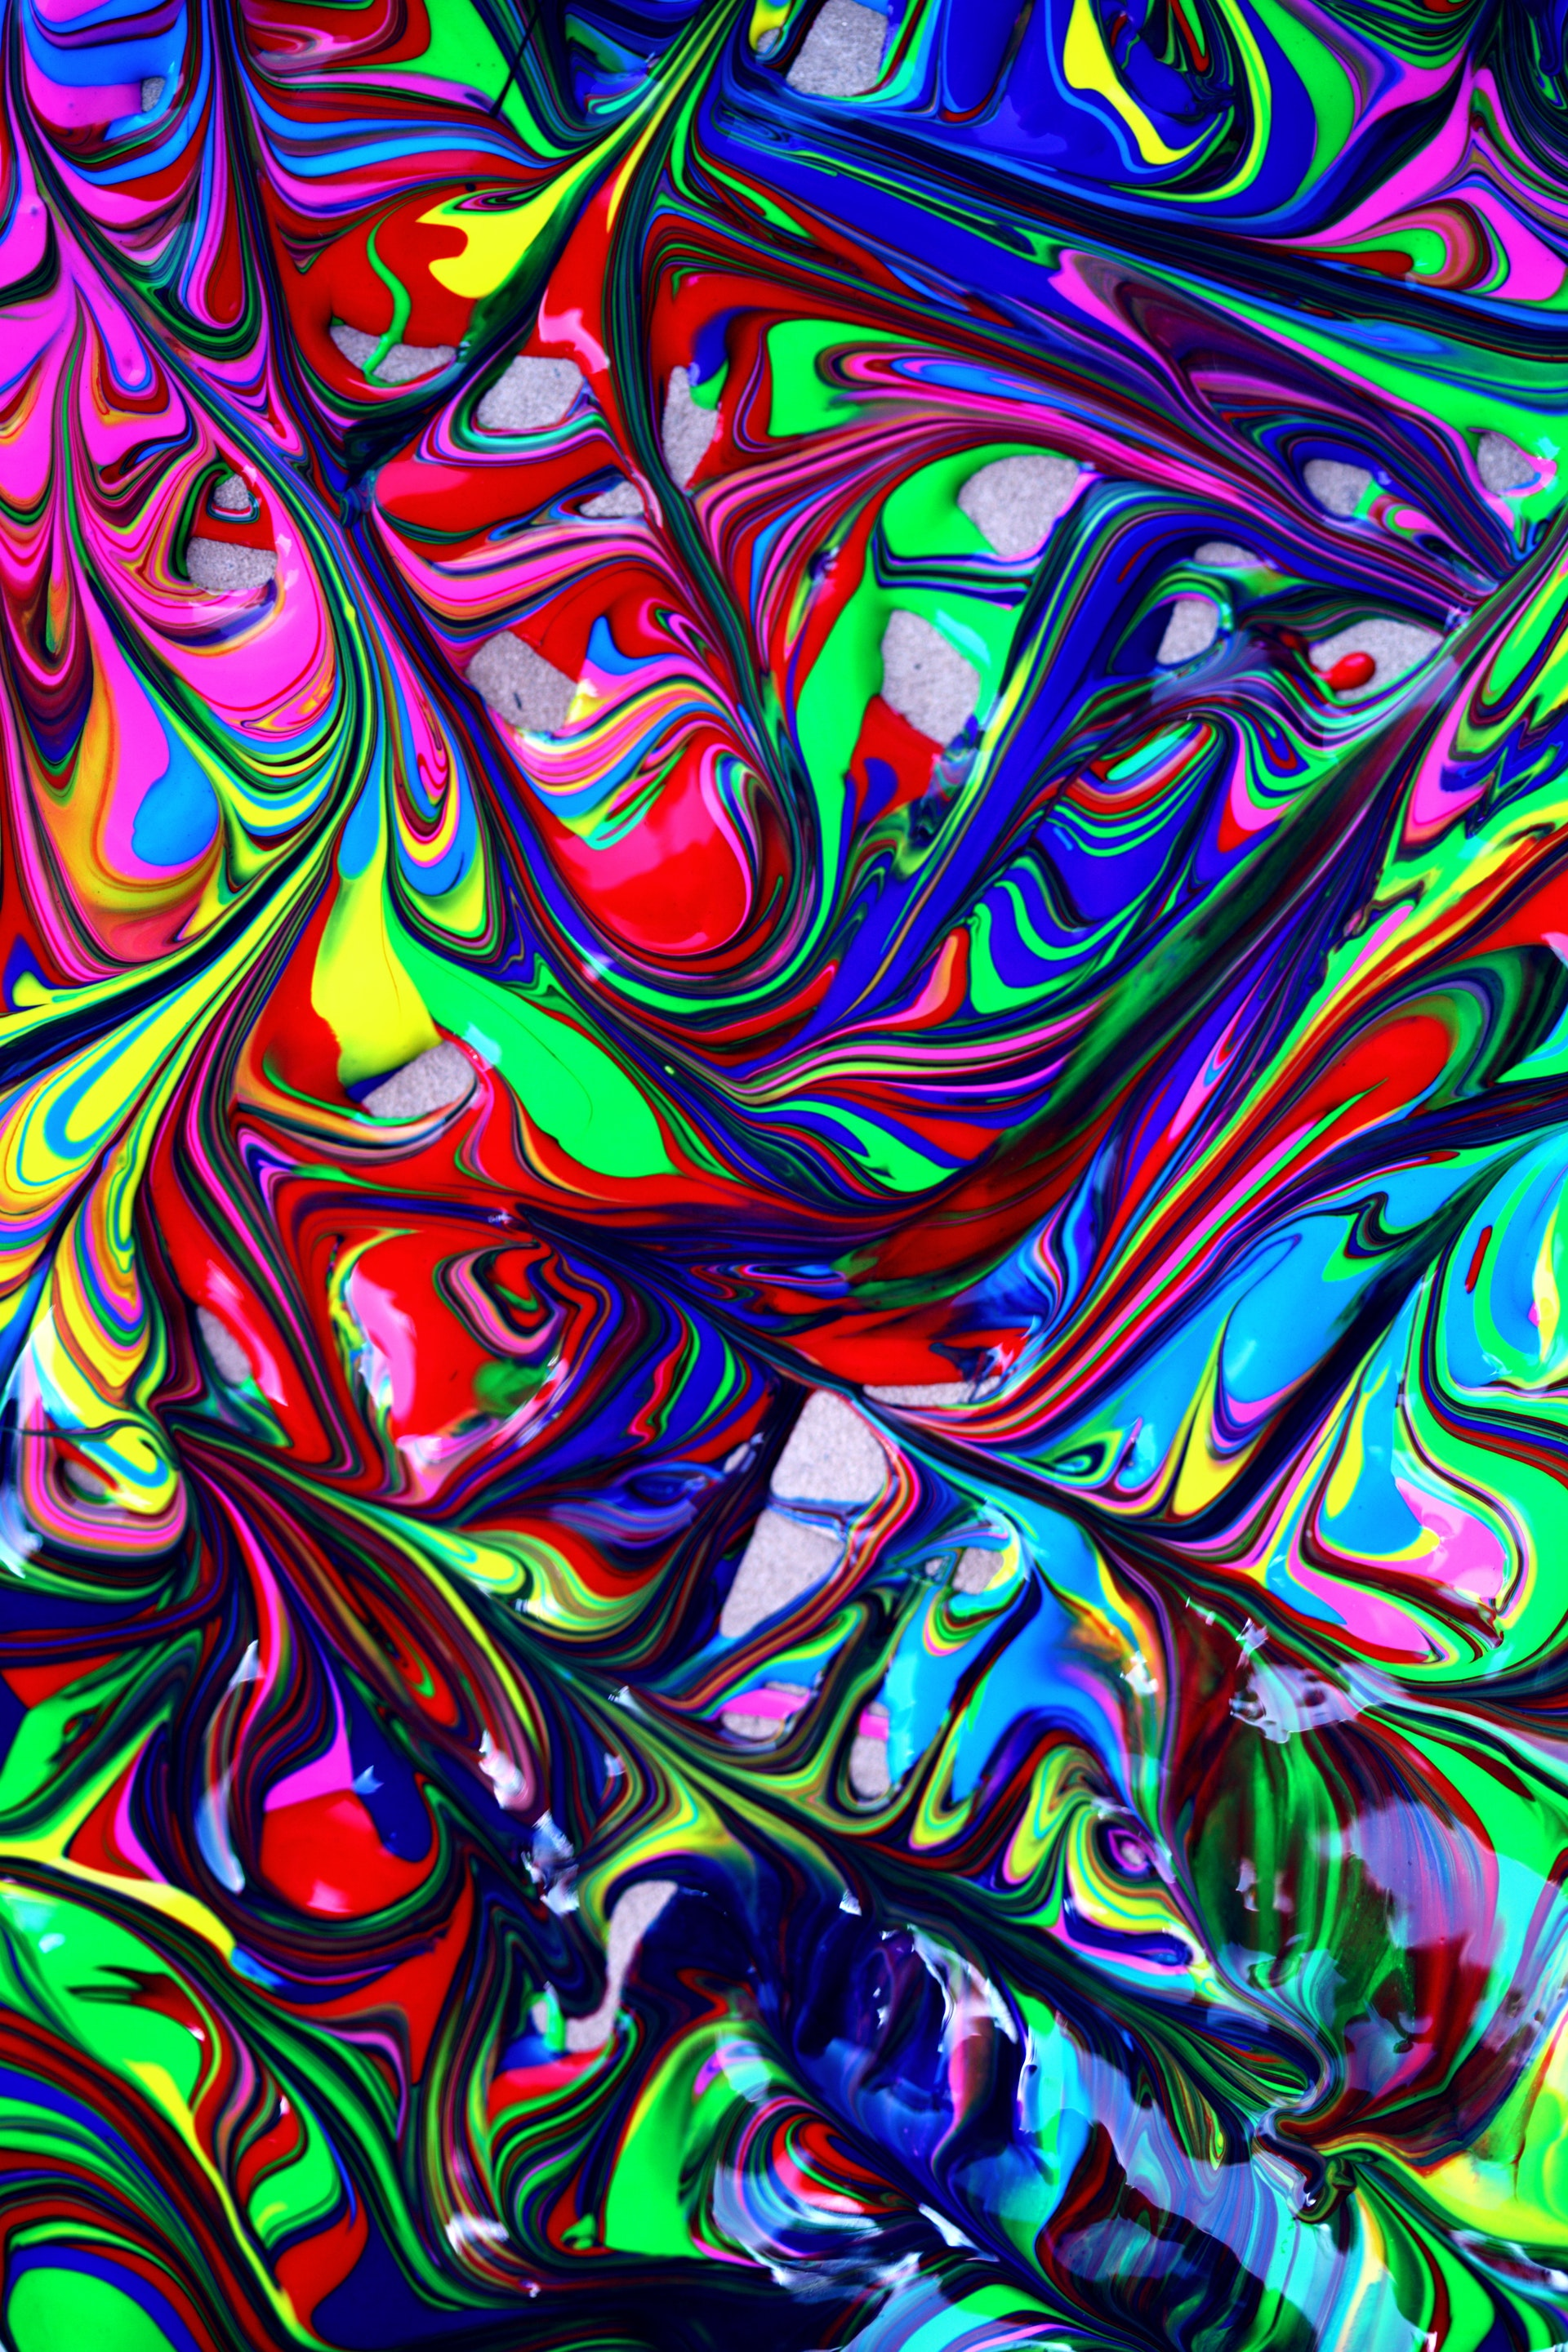
\includegraphics[width=\textwidth]{resources/content/style/multicolored_abstract_artwork.jpg}
    \end{subfigure}
    \begin{subfigure}[h]{0.32\textwidth}
        \centering
        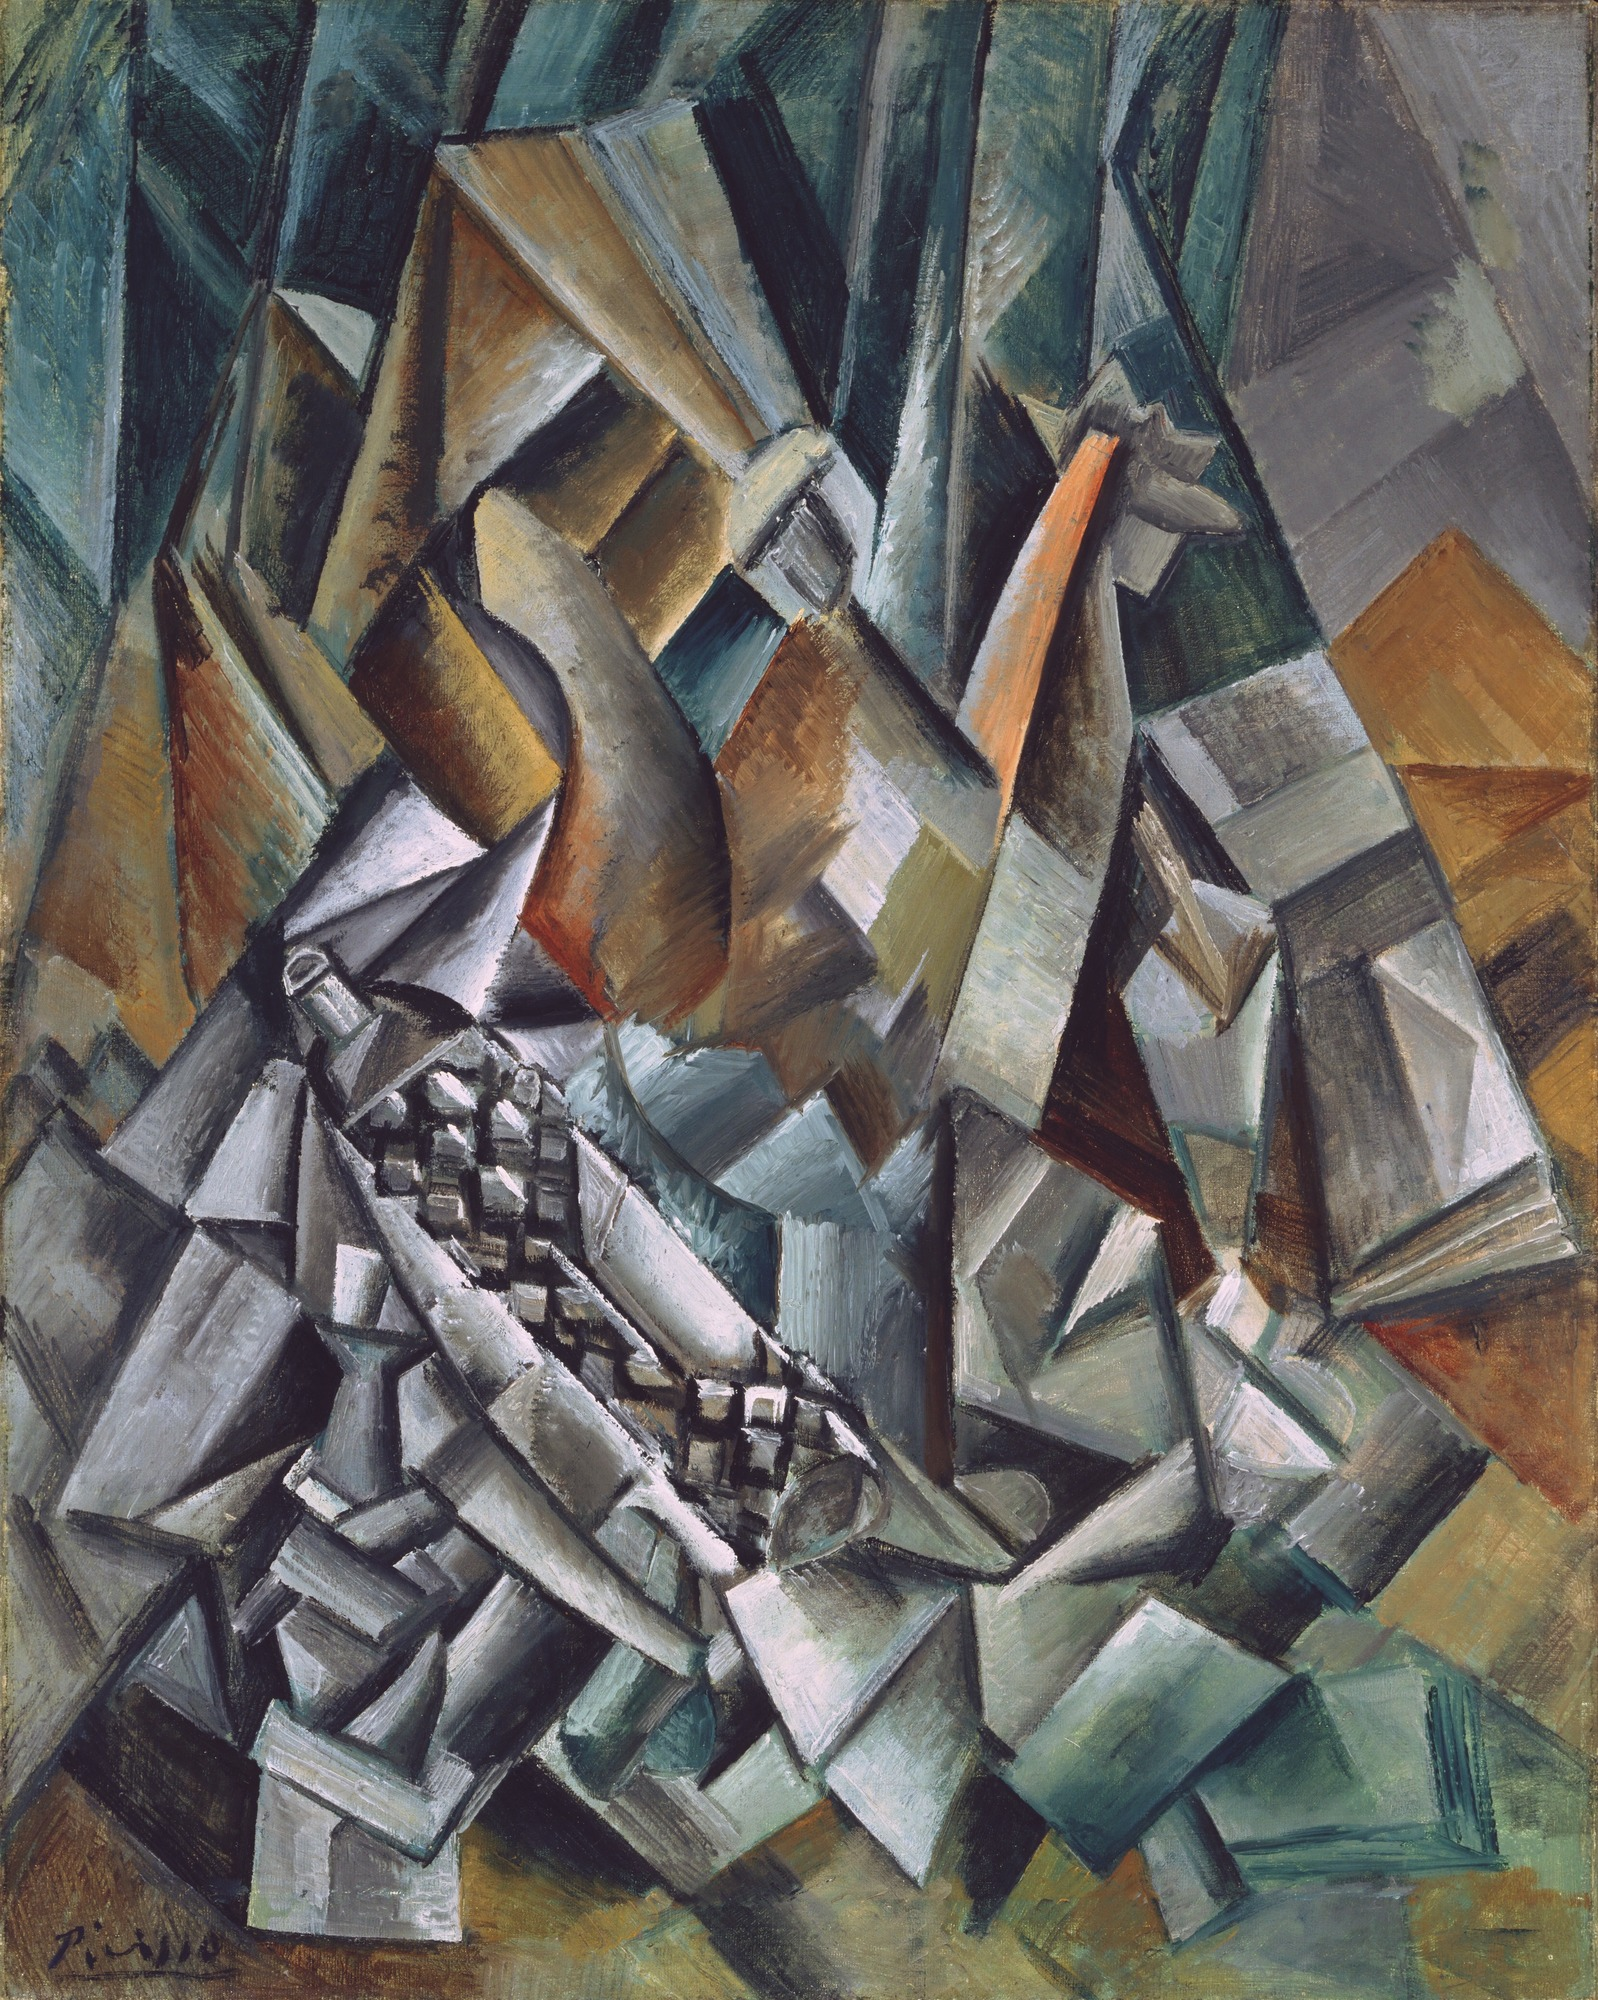
\includegraphics[width=\textwidth]{resources/content/style/still_life_with_liqueur_bottle.jpg}
    \end{subfigure}



    \begin{subfigure}[h]{0.32\textwidth}
        \centering
        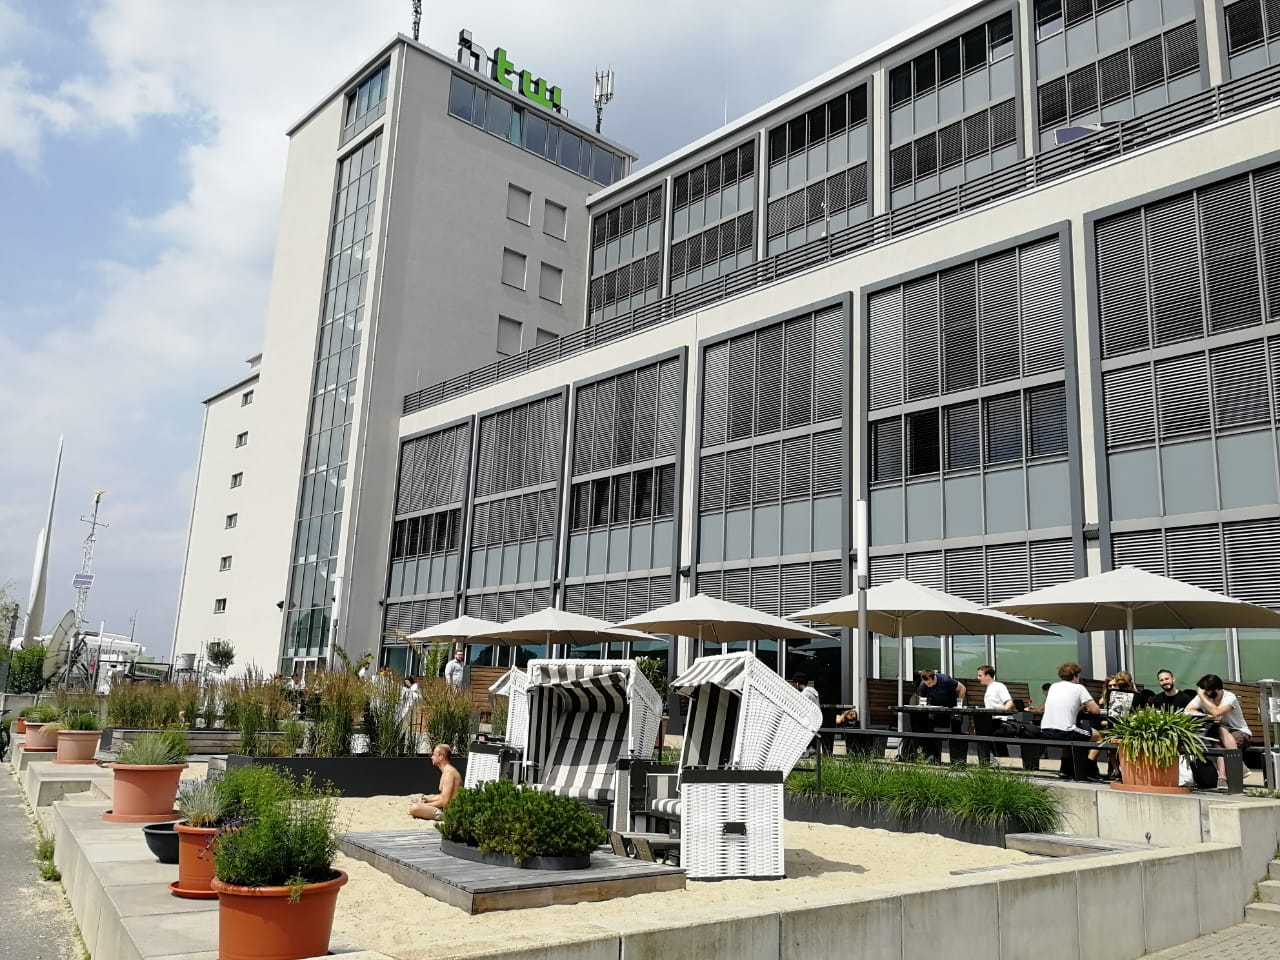
\includegraphics[width=\textwidth]{resources/content/content/htw.jpg}
    \end{subfigure}
    \begin{subfigure}[h]{0.32\textwidth}
        \centering
        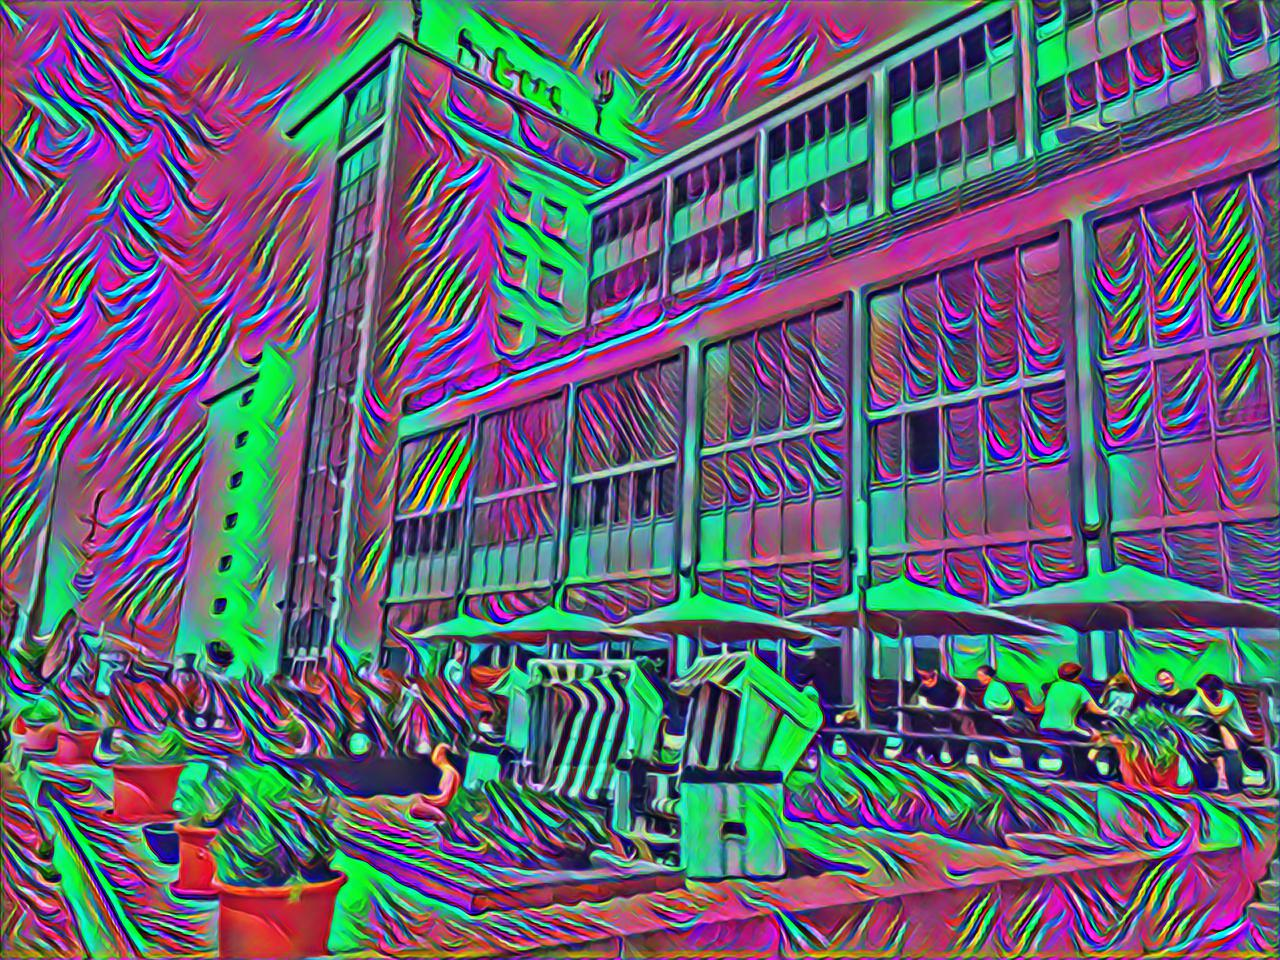
\includegraphics[width=\textwidth]{resources/content/experiments/htw-vgg16_multicolored_abstract_artwork.jpg}
    \end{subfigure}
    \begin{subfigure}[h]{0.32\textwidth}
        \centering
        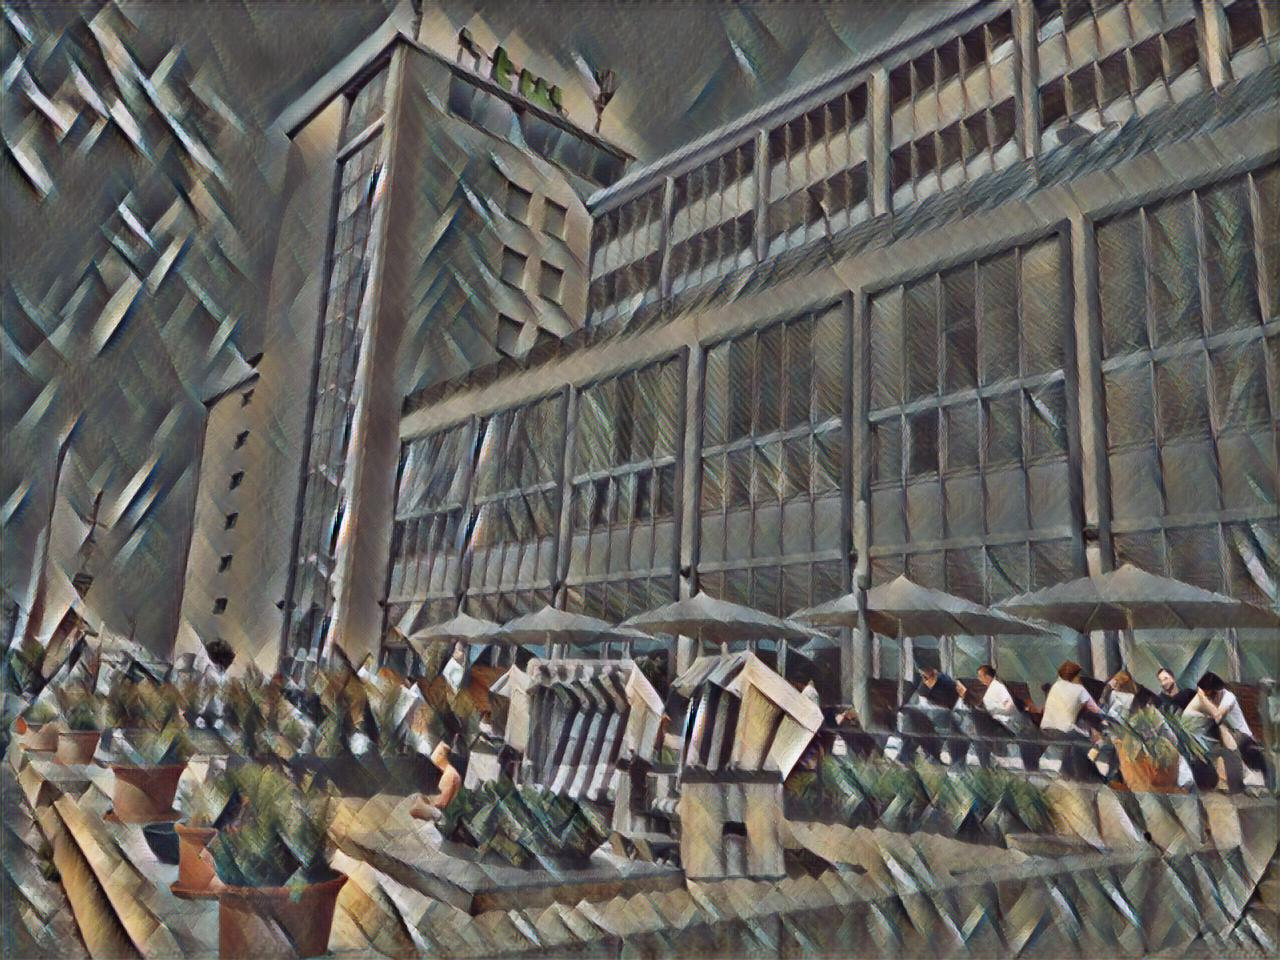
\includegraphics[width=\textwidth]{resources/content/experiments/htw-vgg16_still_life_with_liqueur_bottle.jpg}
    \end{subfigure}


    \begin{subfigure}[h]{0.32\textwidth}
        \centering
        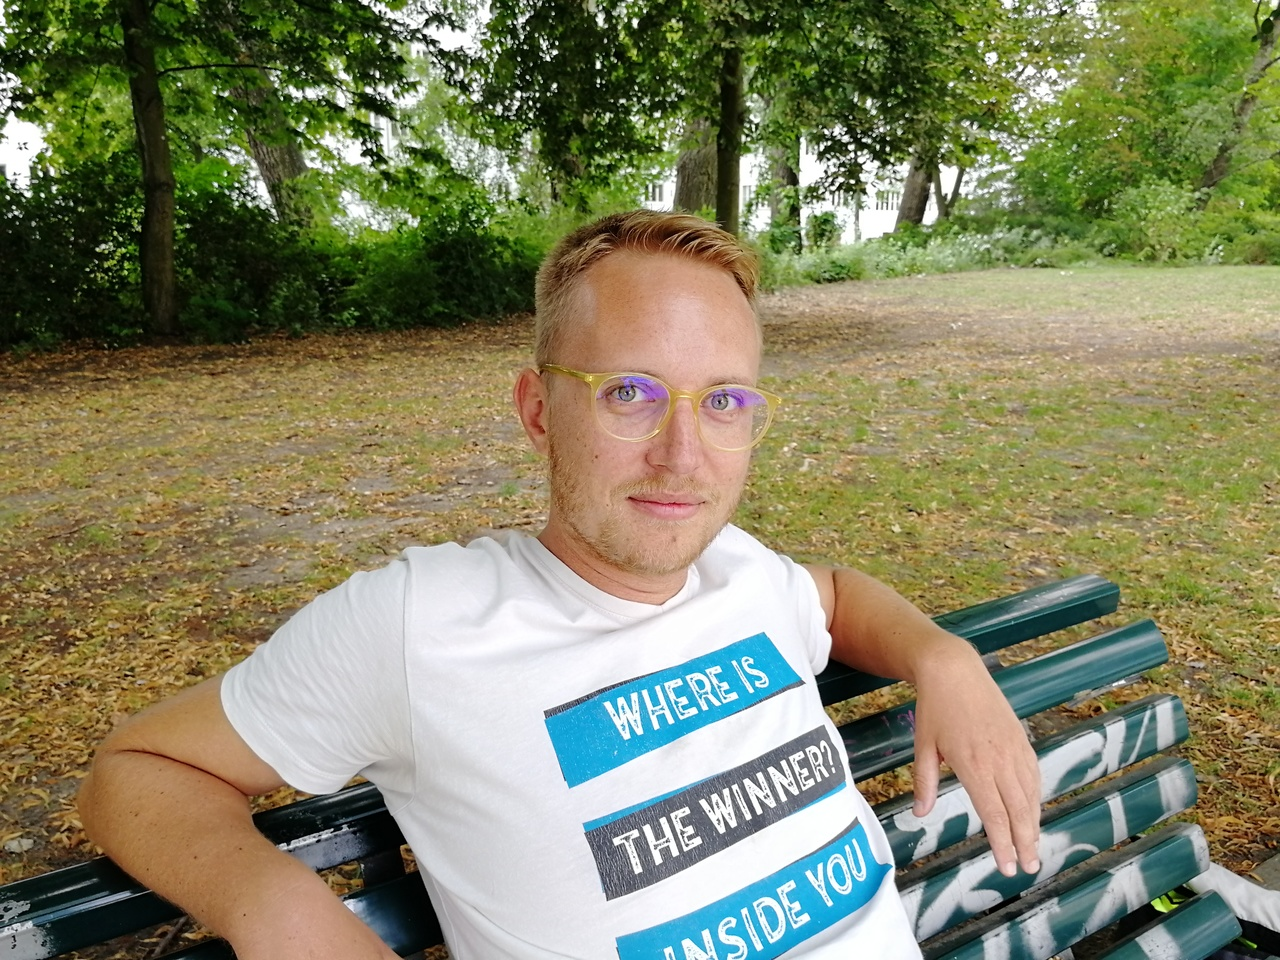
\includegraphics[width=\textwidth]{resources/content/content/ich.jpg}
    \end{subfigure}
    \begin{subfigure}[h]{0.32\textwidth}
        \centering
        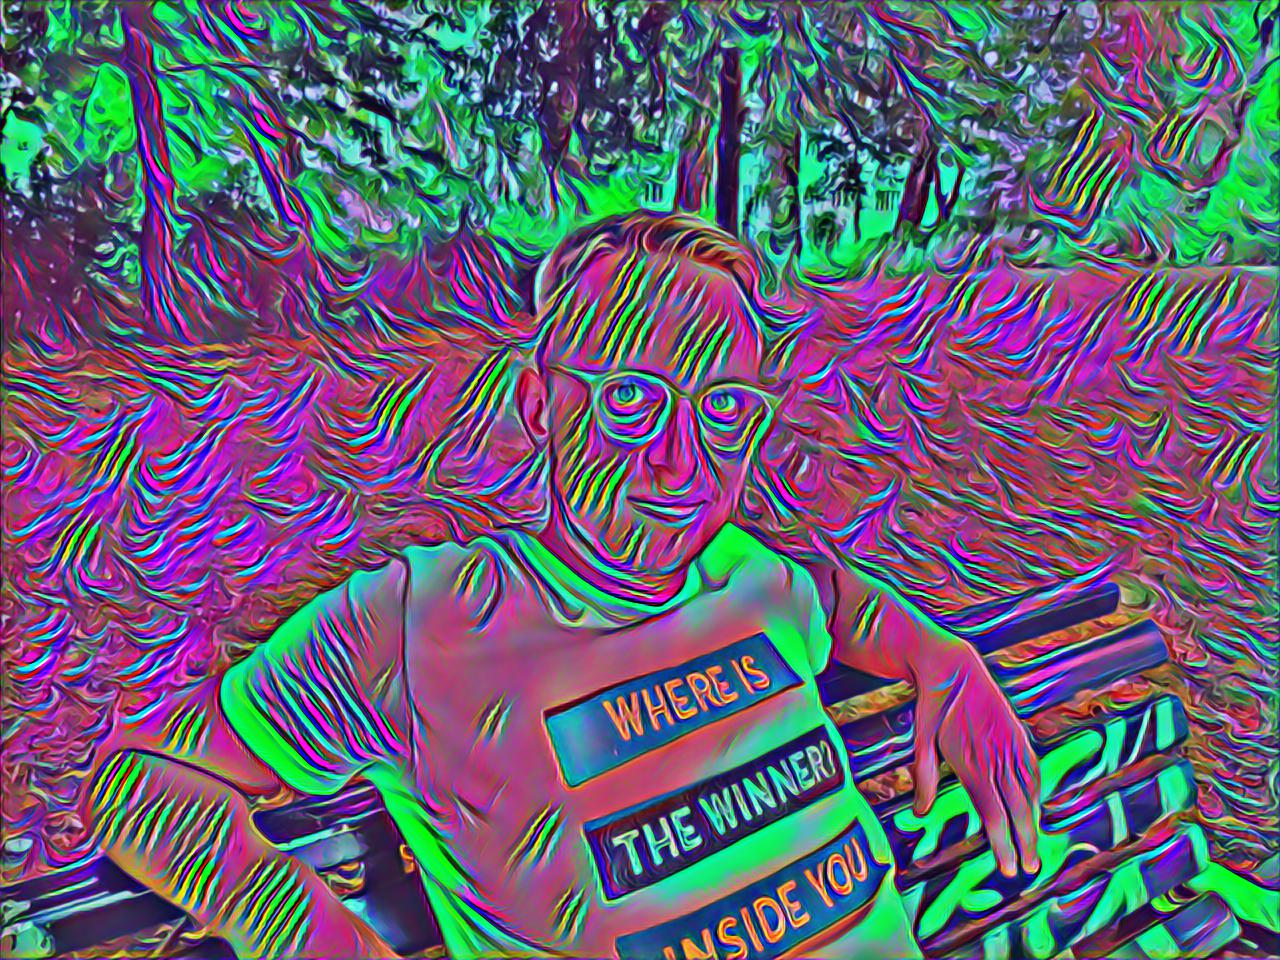
\includegraphics[width=\textwidth]{resources/content/experiments/ich-vgg16_multicolored_abstract_artwork.jpg}
    \end{subfigure}
    \begin{subfigure}[h]{0.32\textwidth}
        \centering
        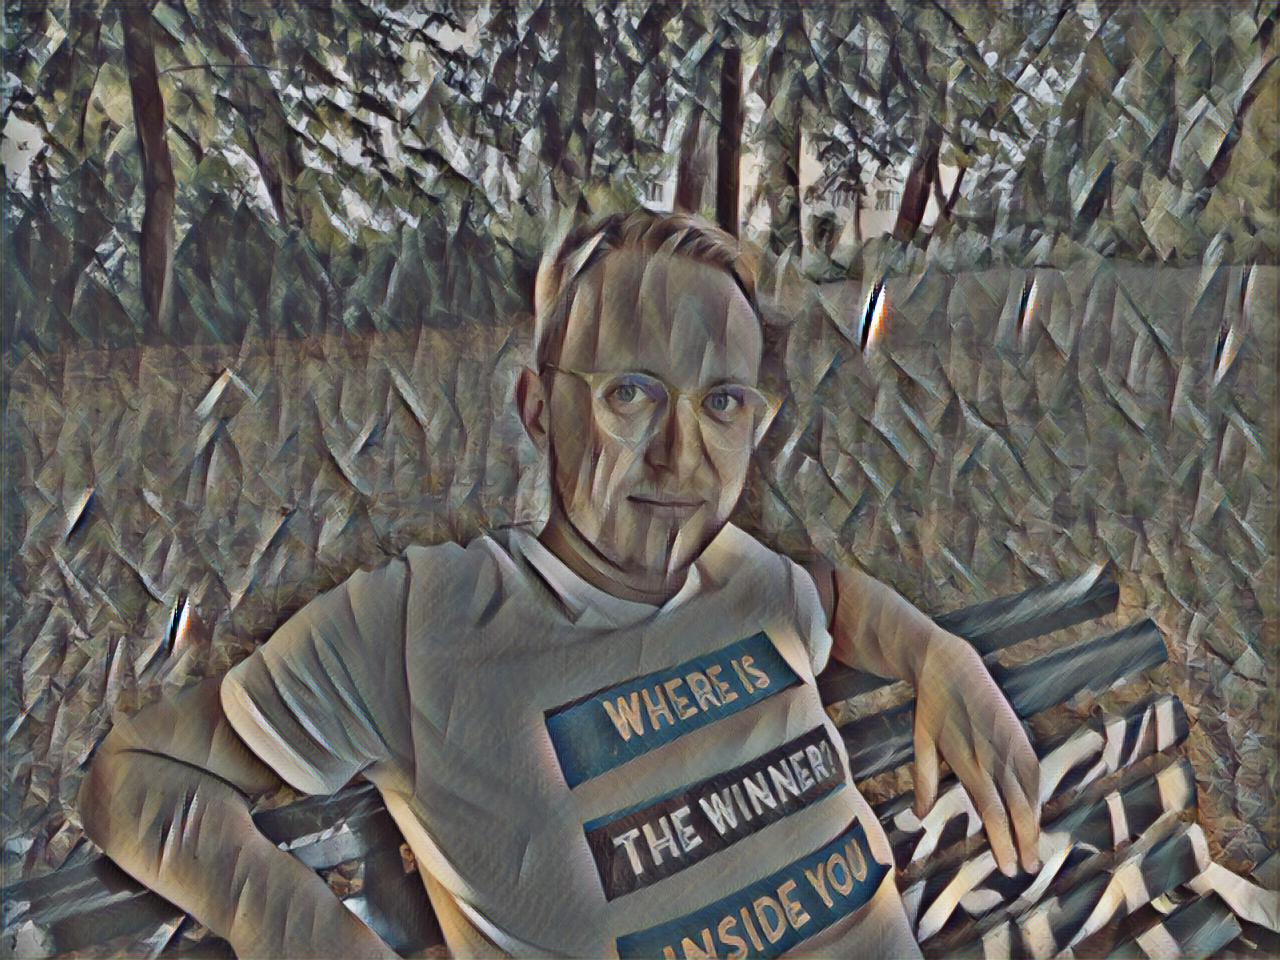
\includegraphics[width=\textwidth]{resources/content/experiments/ich-vgg16_still_life_with_liqueur_bottle.jpg}
    \end{subfigure}



    \begin{subfigure}[h]{0.32\textwidth}
        \centering
        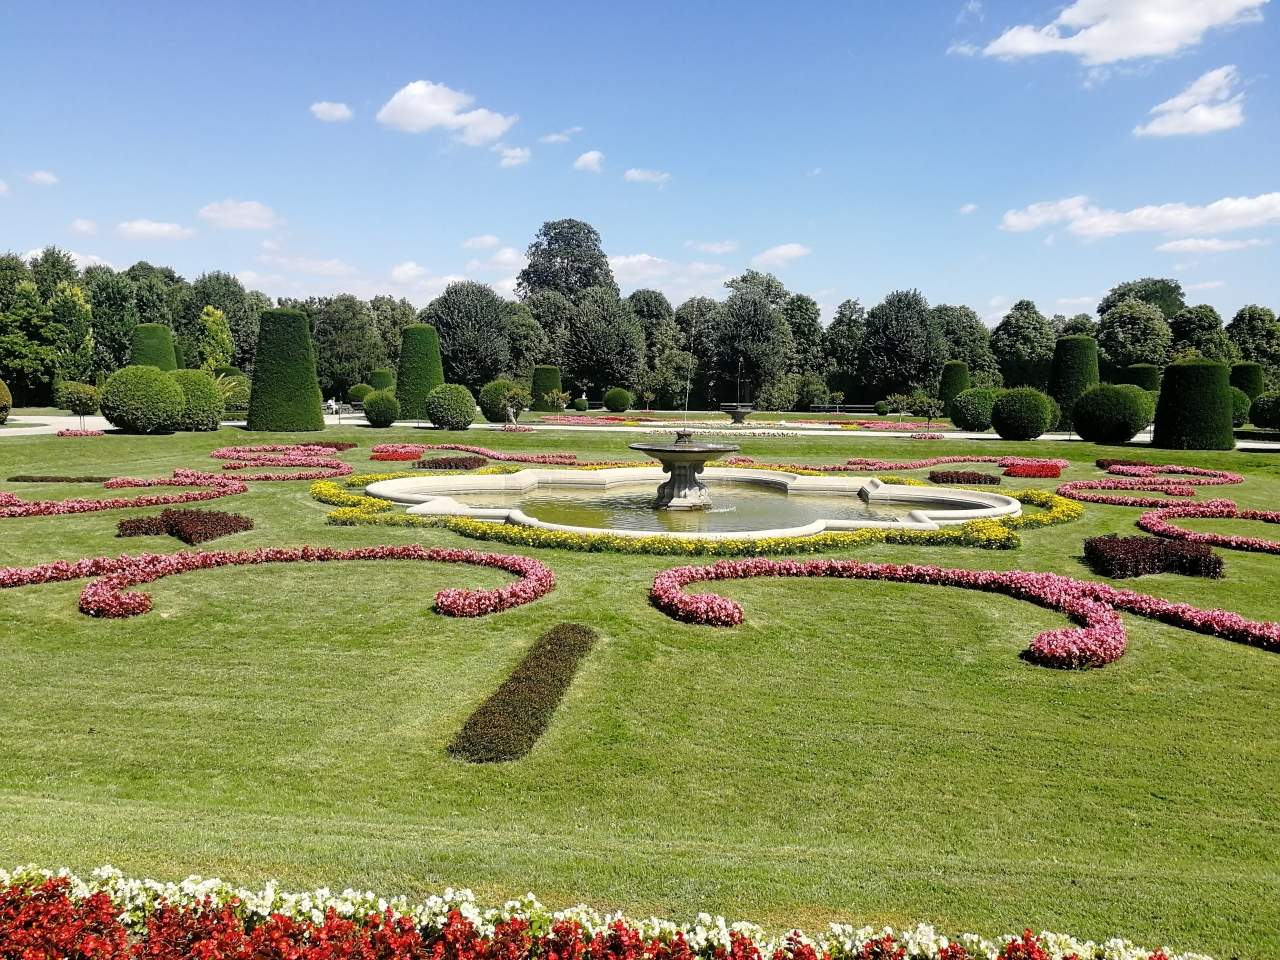
\includegraphics[width=\textwidth]{resources/content/content/garden.jpg}
    \end{subfigure}
    \begin{subfigure}[h]{0.32\textwidth}
        \centering
        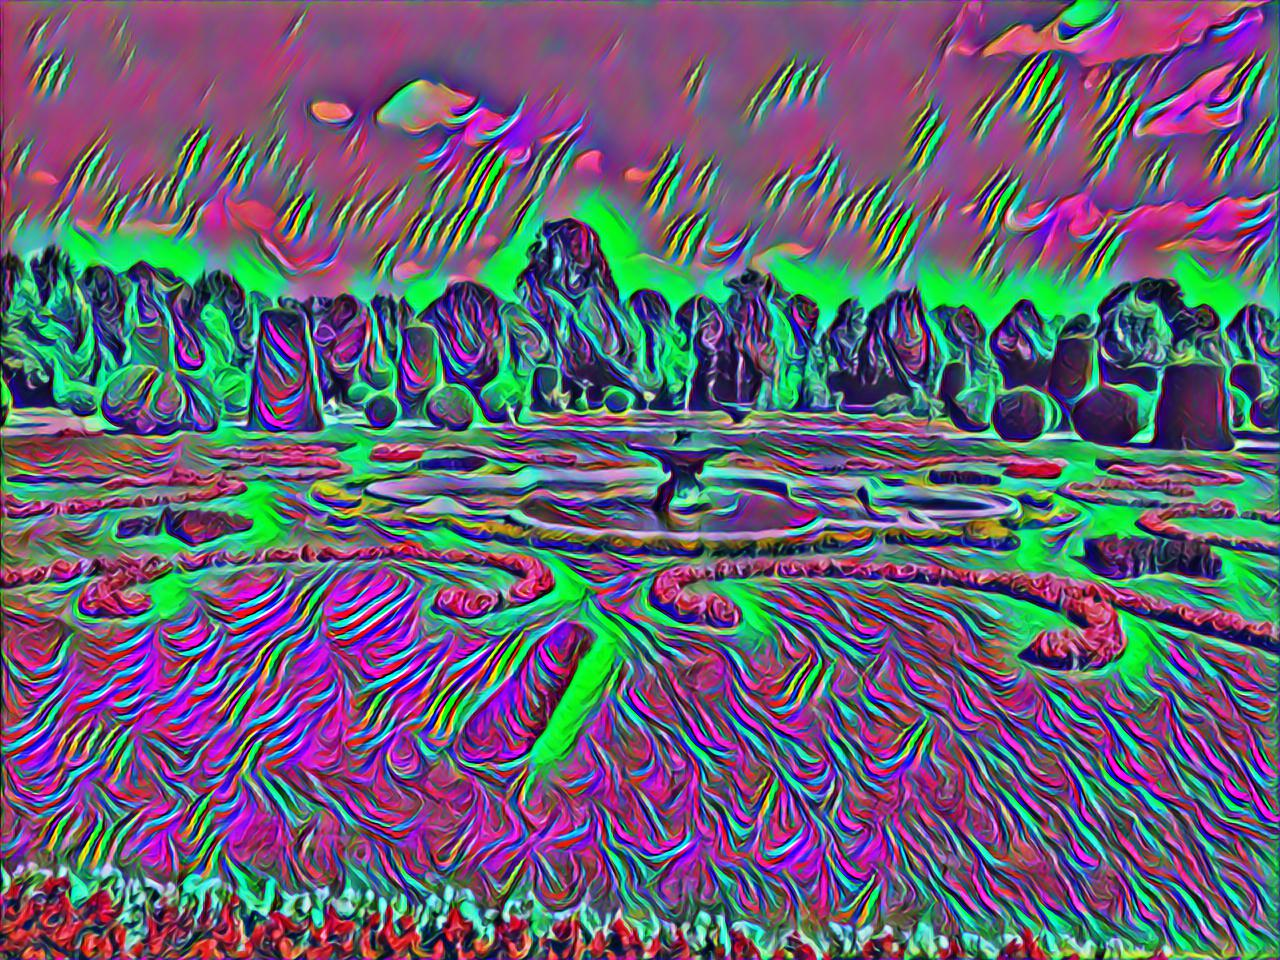
\includegraphics[width=\textwidth]{resources/content/experiments/garden-vgg16_multicolored_abstract_artwork.jpg}
    \end{subfigure}
    \begin{subfigure}[h]{0.32\textwidth}
        \centering
        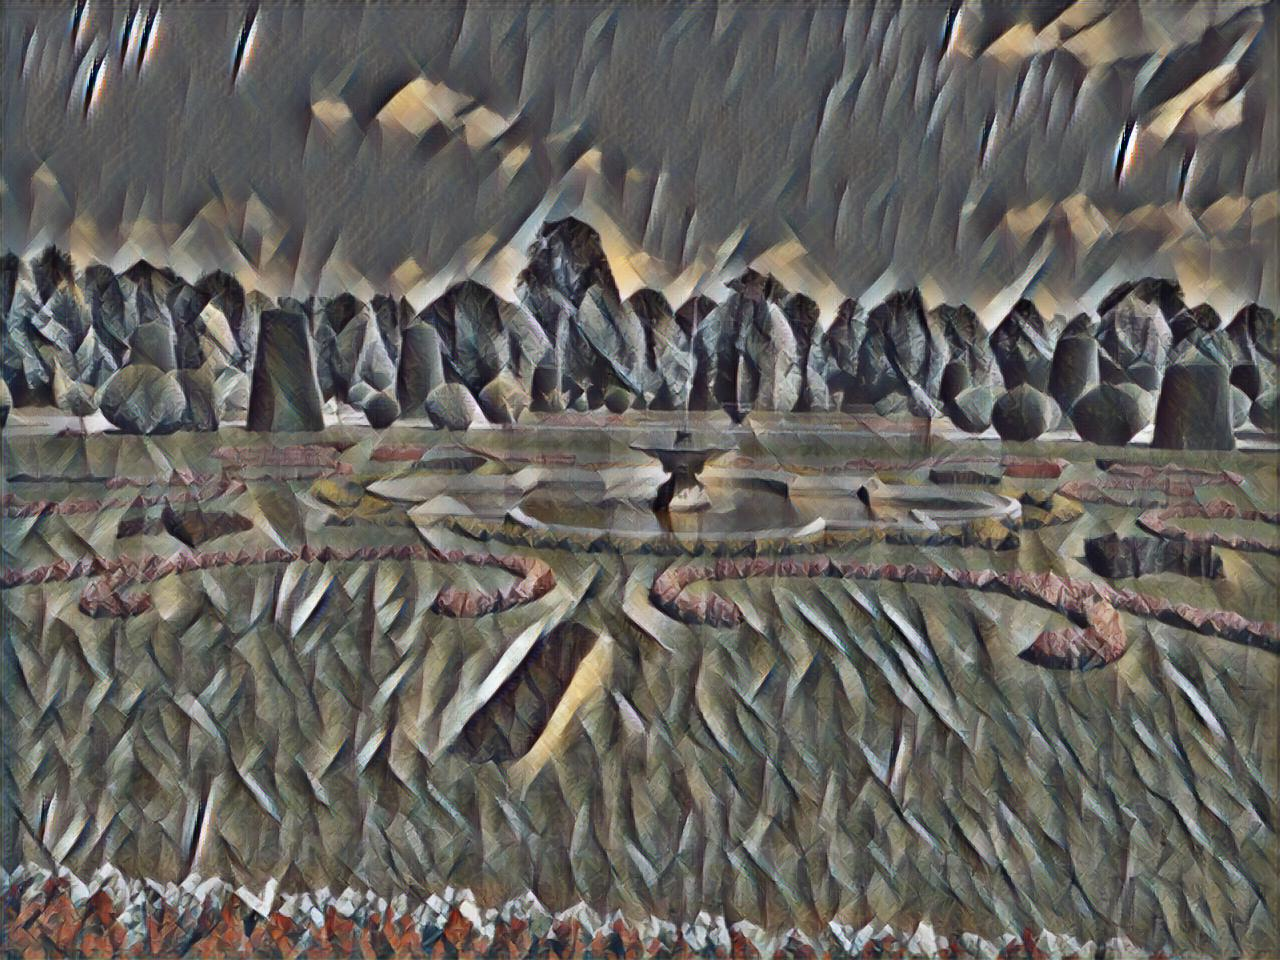
\includegraphics[width=\textwidth]{resources/content/experiments/garden-vgg16_still_life_with_liqueur_bottle.jpg}
    \end{subfigure}

    \caption{Eigene Abbildungen kombiniert mit verschiedenen Stilen: \cite{multicolored_abstract_artwork_img}, \cite{still_life_with_liqueur_bottle_img}}
    \label{img:trained_models2}
\end{figure}



\begin{figure}[H]
    \centering

    \begin{subfigure}[h]{0.32\textwidth}
        \centering
        \quad
    \end{subfigure}
    \begin{subfigure}[h]{0.32\textwidth}
        \centering
        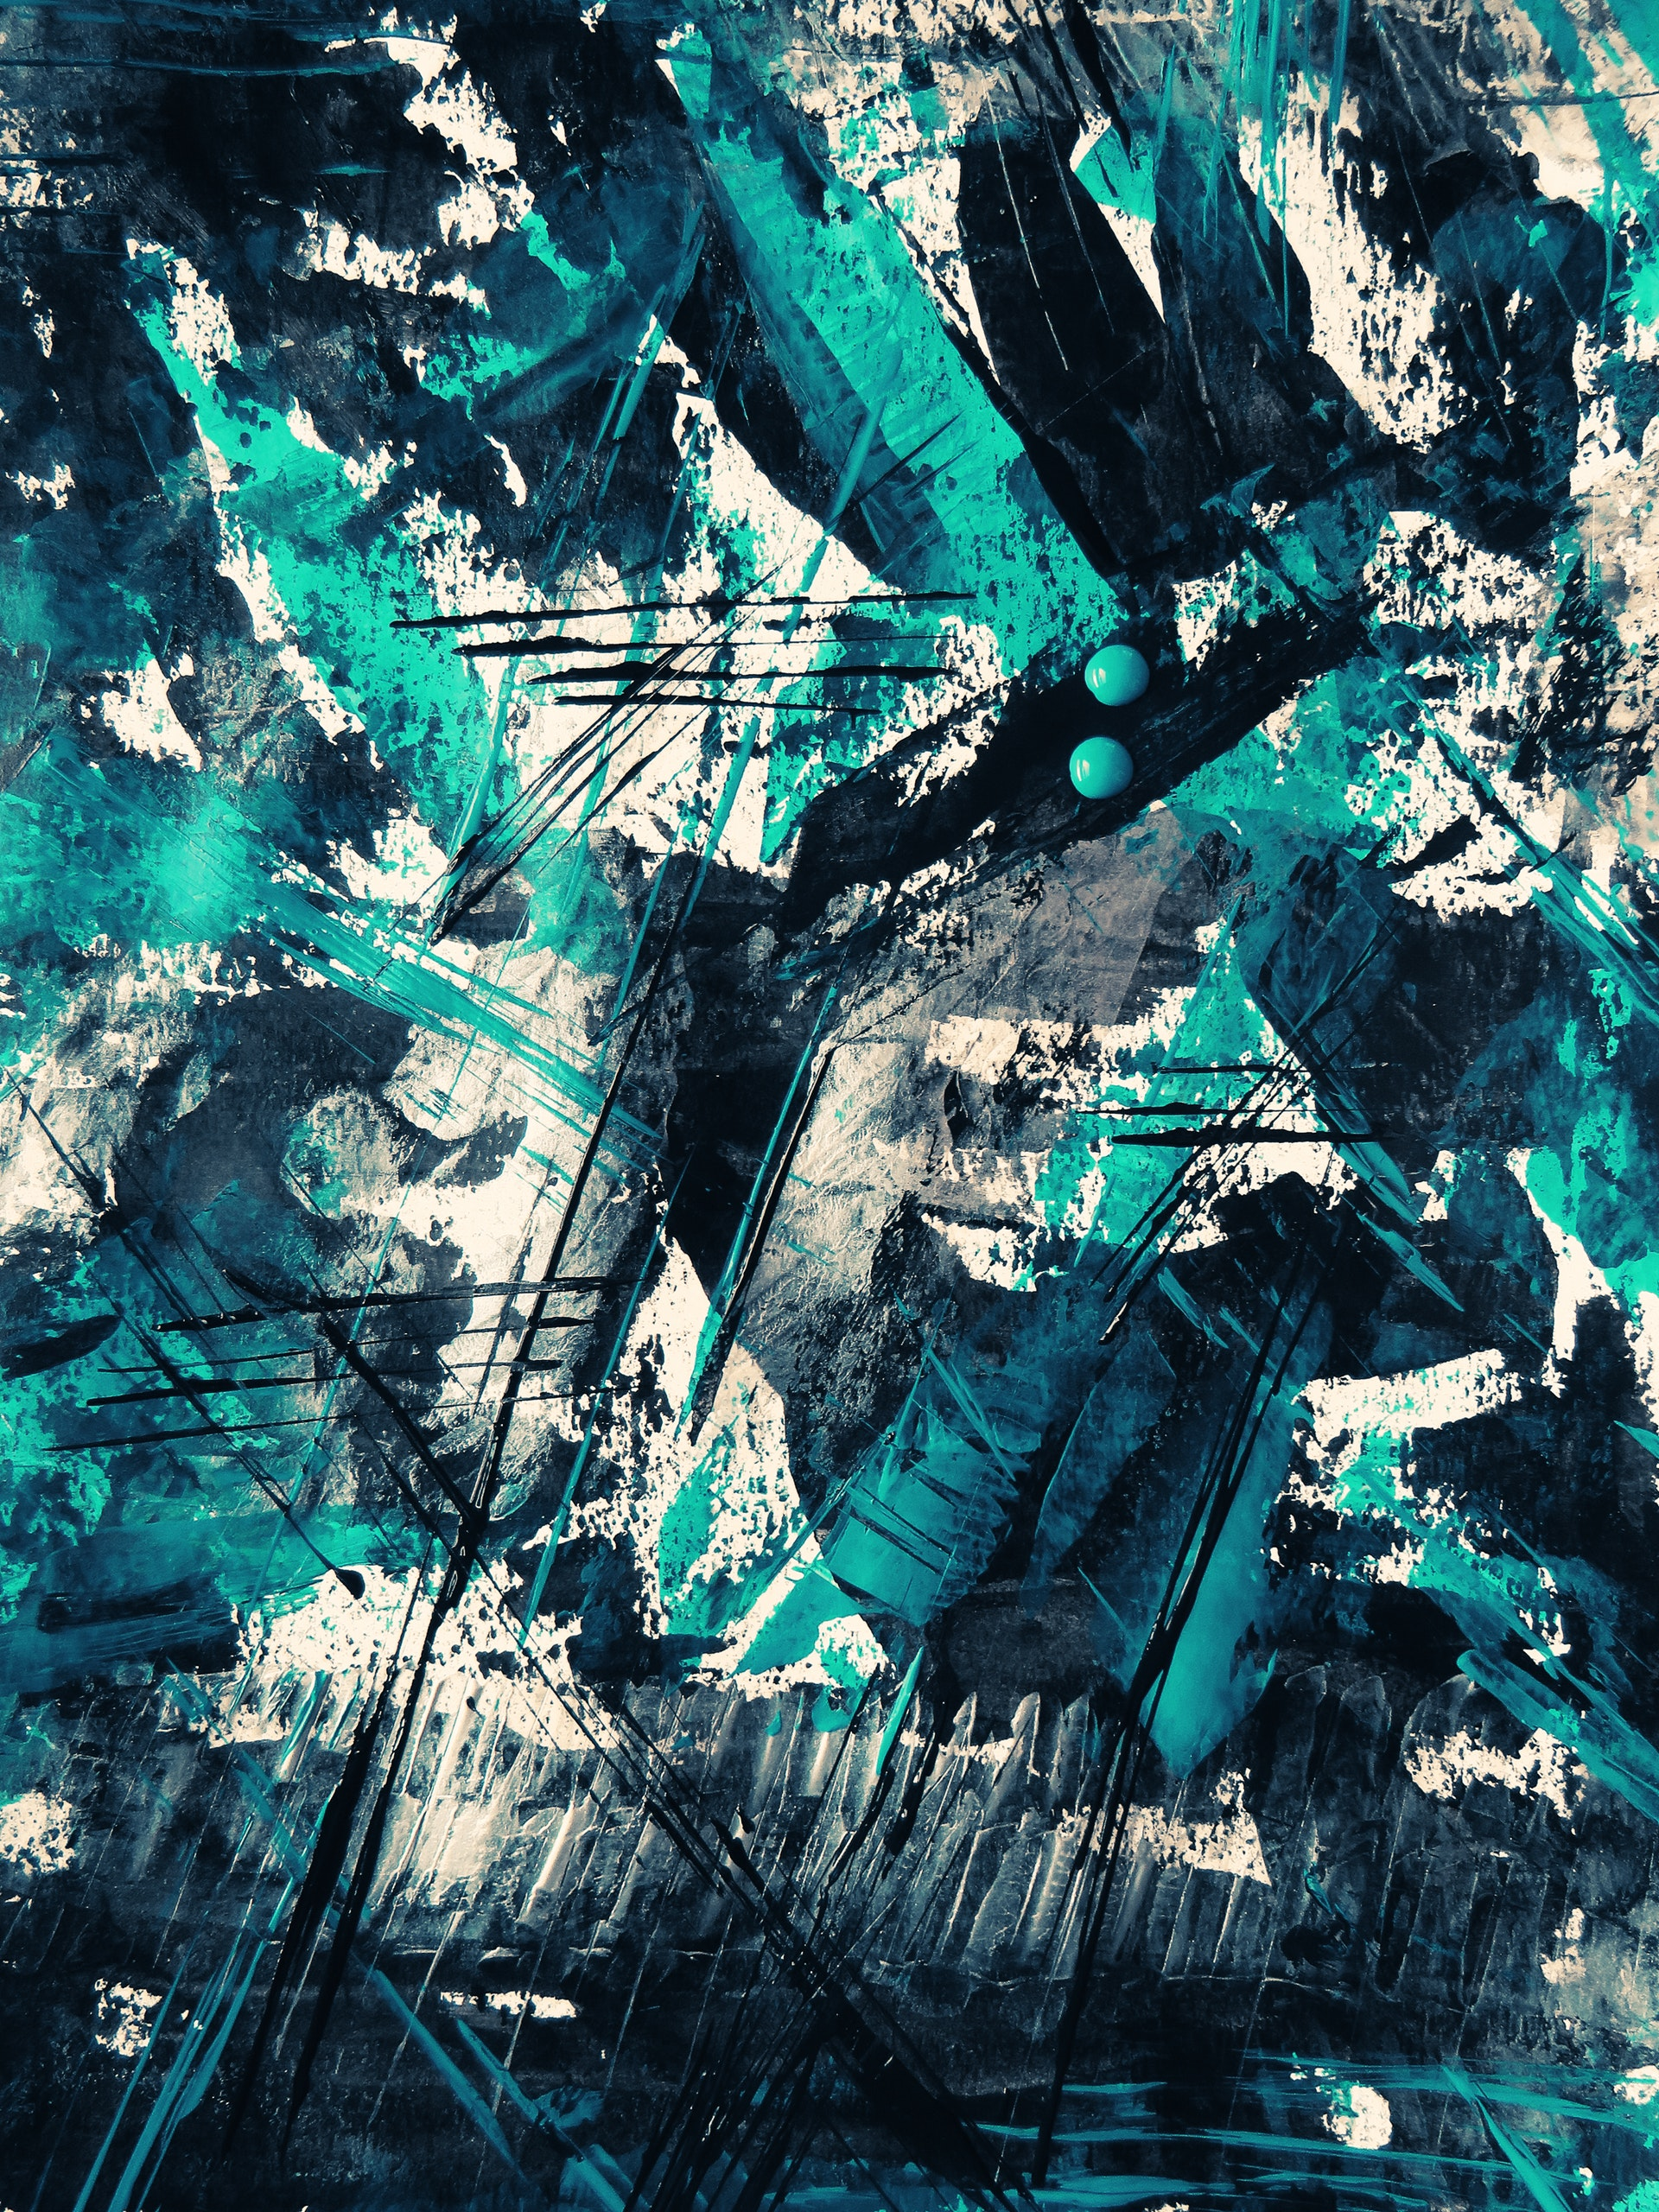
\includegraphics[width=\textwidth]{resources/content/style/teal_and_black_abstract_painting.jpg}
    \end{subfigure}
    \begin{subfigure}[h]{0.32\textwidth}
        \centering
        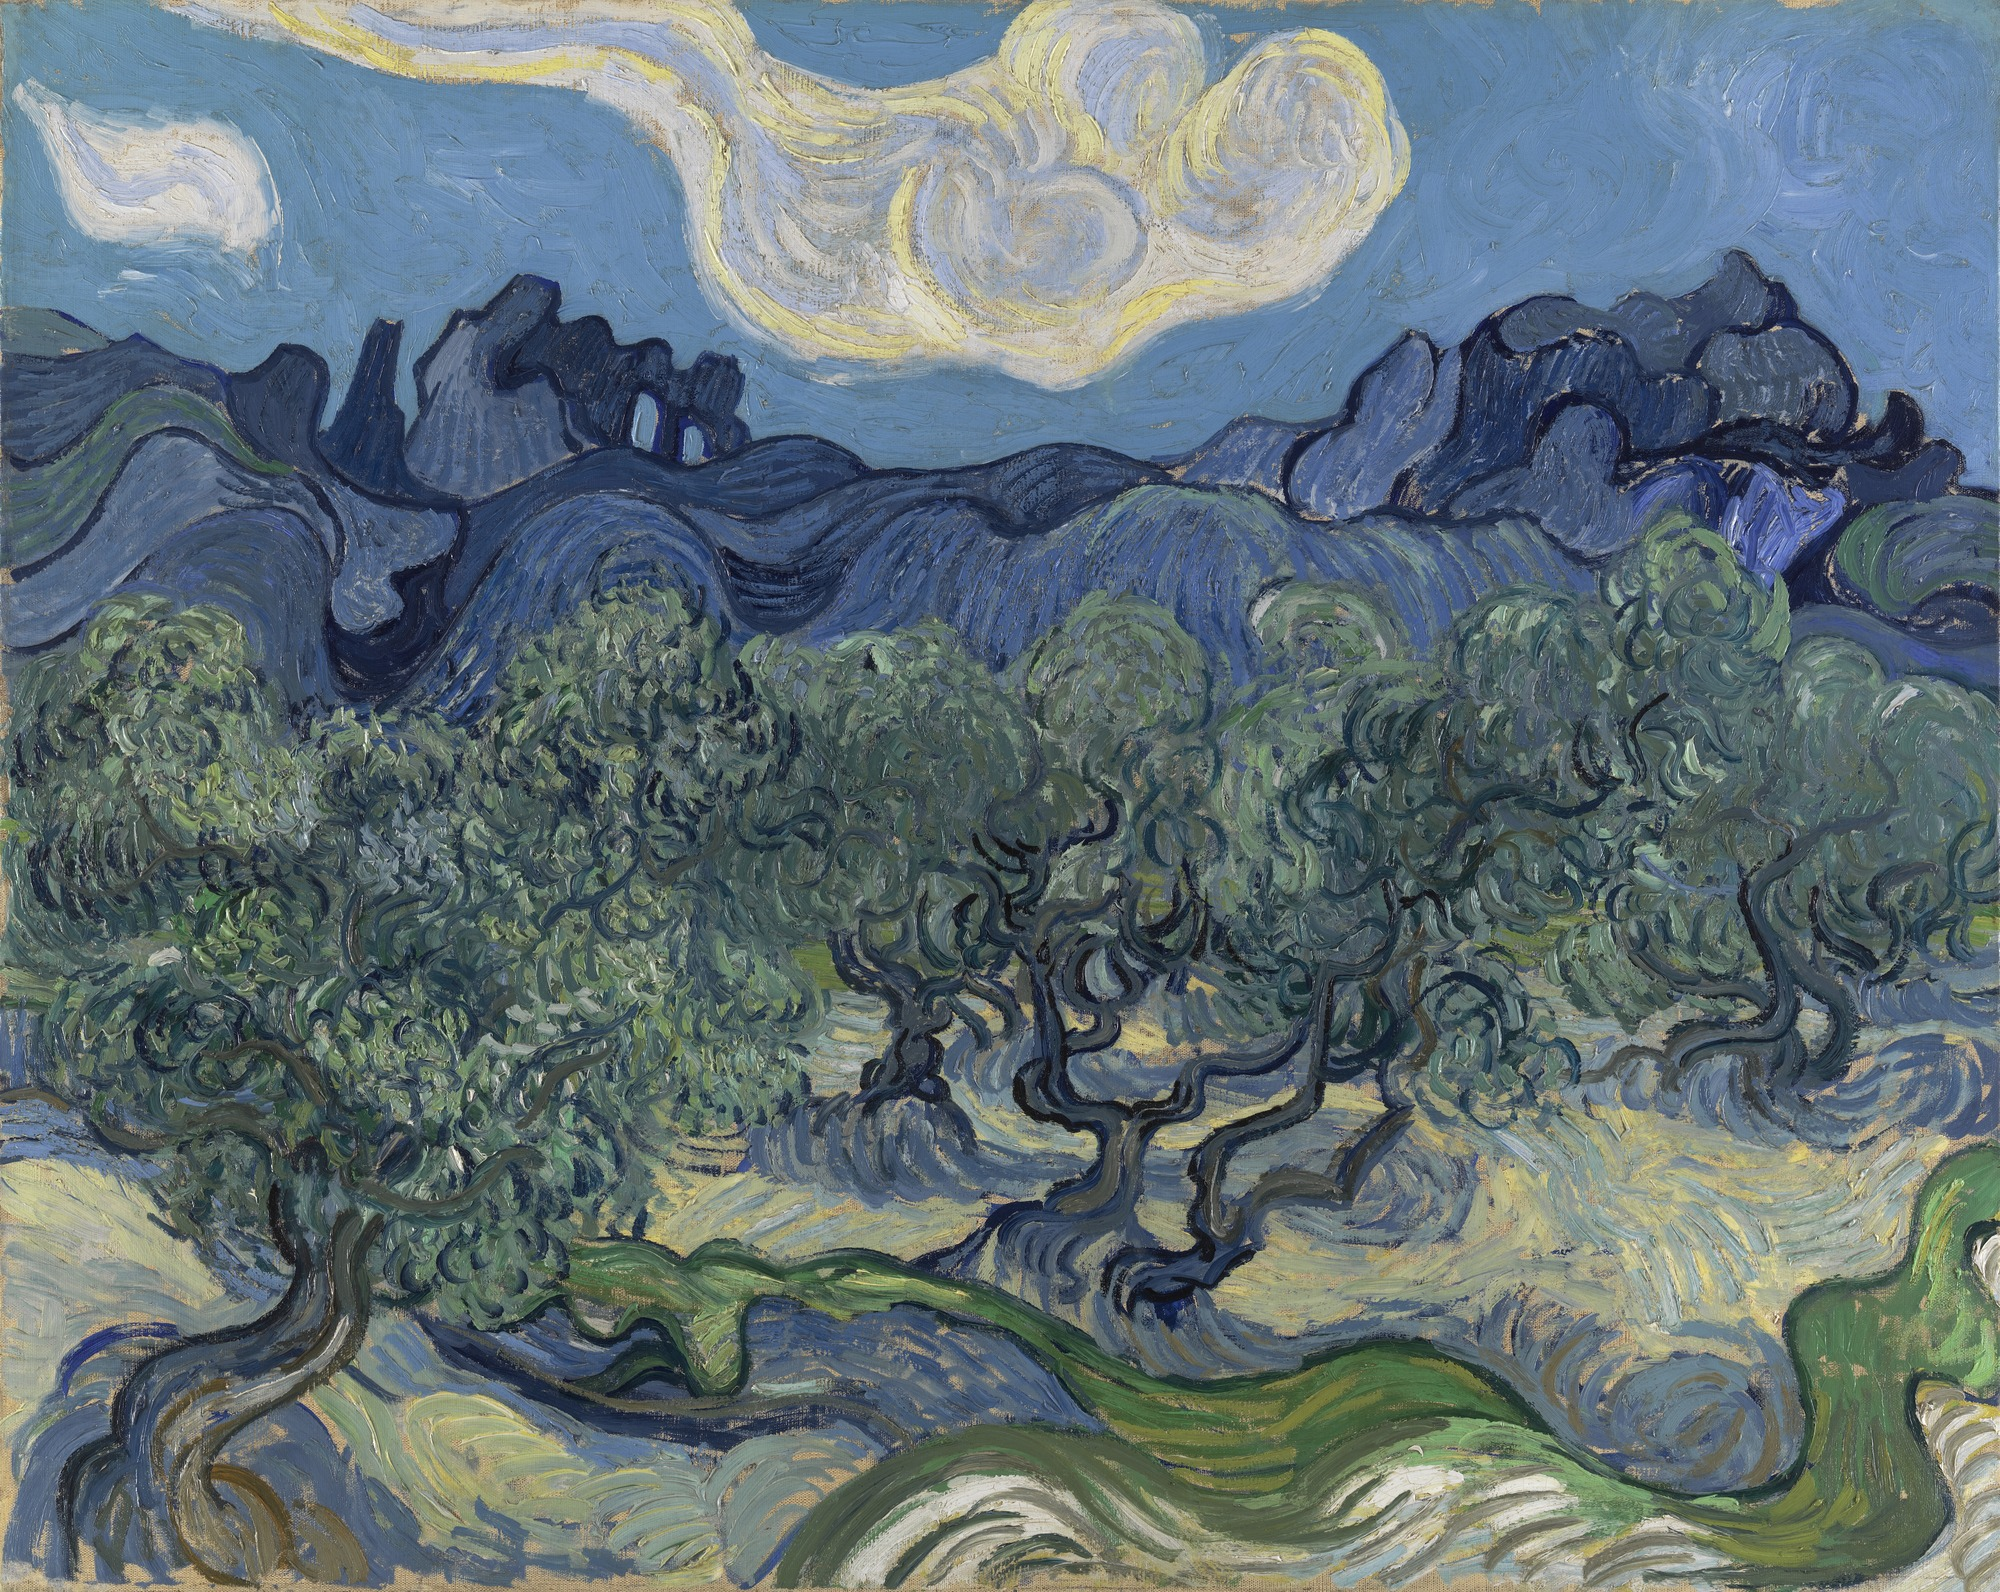
\includegraphics[width=\textwidth]{resources/content/style/the_olive_trees.jpg}
    \end{subfigure}



    \begin{subfigure}[h]{0.32\textwidth}
        \centering
        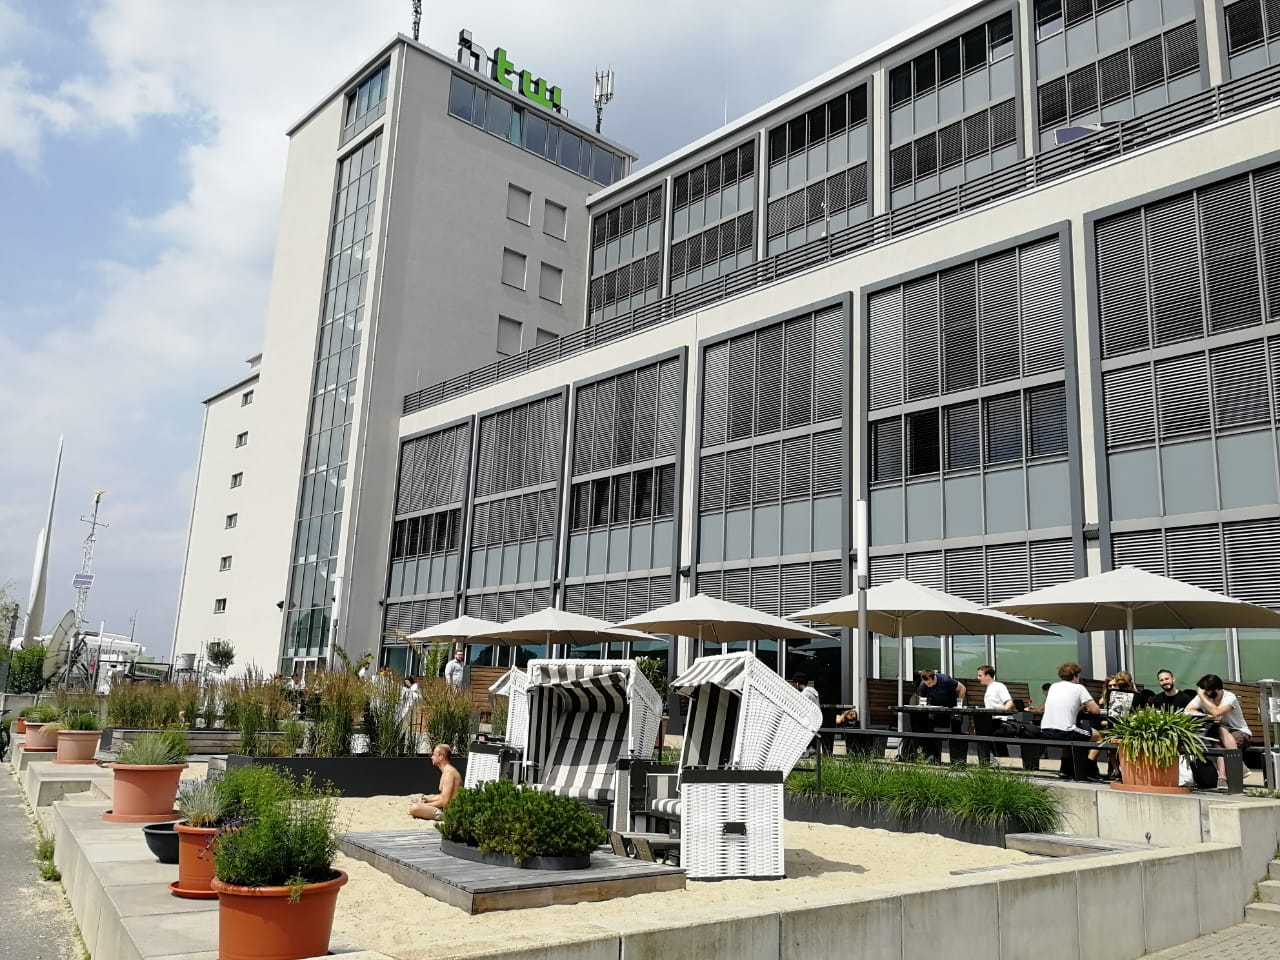
\includegraphics[width=\textwidth]{resources/content/content/htw.jpg}
    \end{subfigure}
    \begin{subfigure}[h]{0.32\textwidth}
        \centering
        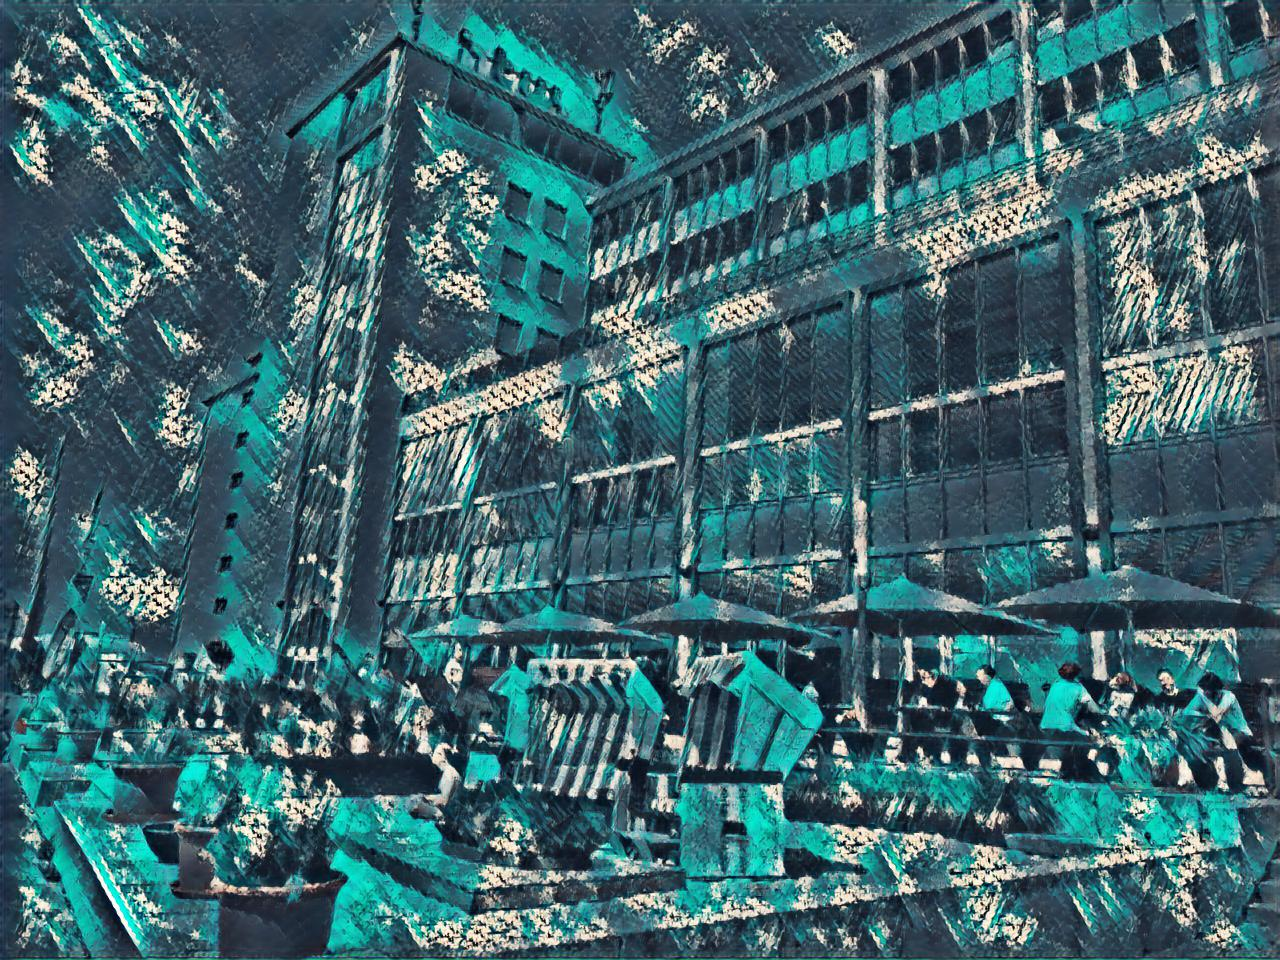
\includegraphics[width=\textwidth]{resources/content/experiments/htw-vgg16_teal_and_black_abstract_painting.jpg}
    \end{subfigure}
    \begin{subfigure}[h]{0.32\textwidth}
        \centering
        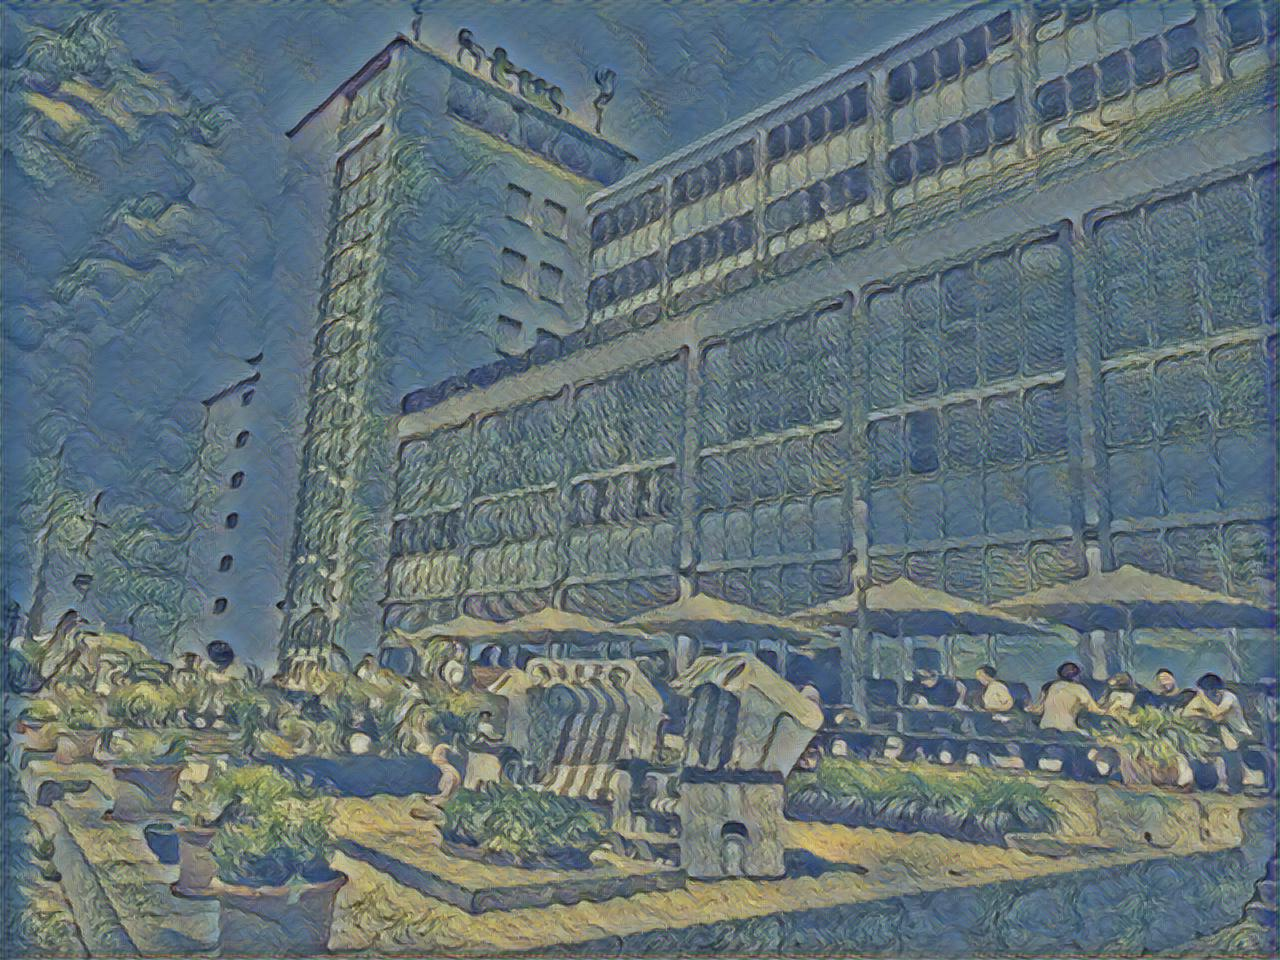
\includegraphics[width=\textwidth]{resources/content/experiments/htw-vgg16_the_olive_trees.jpg}
    \end{subfigure}


    \begin{subfigure}[h]{0.32\textwidth}
        \centering
        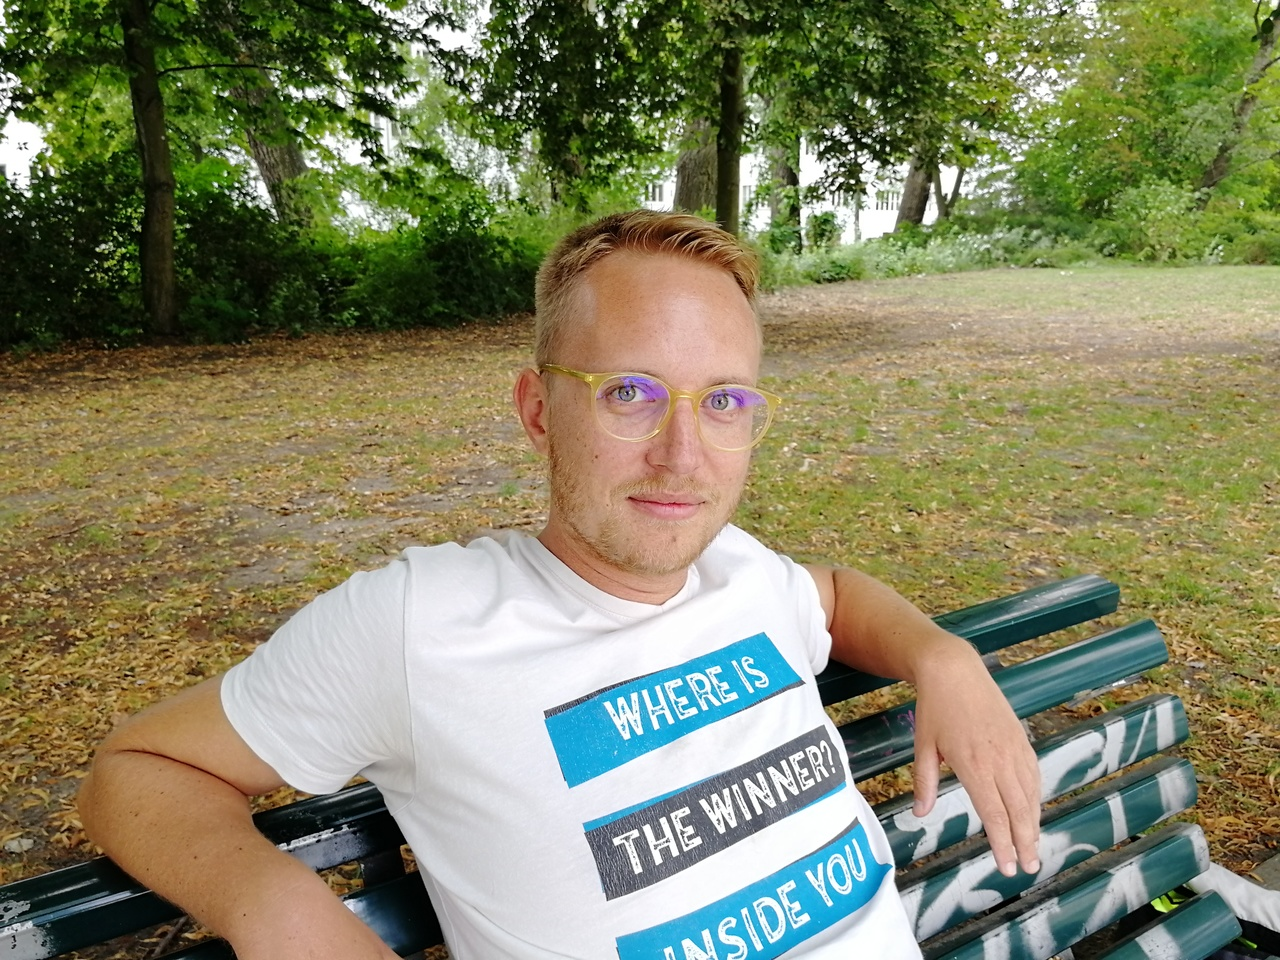
\includegraphics[width=\textwidth]{resources/content/content/ich.jpg}
    \end{subfigure}
    \begin{subfigure}[h]{0.32\textwidth}
        \centering
        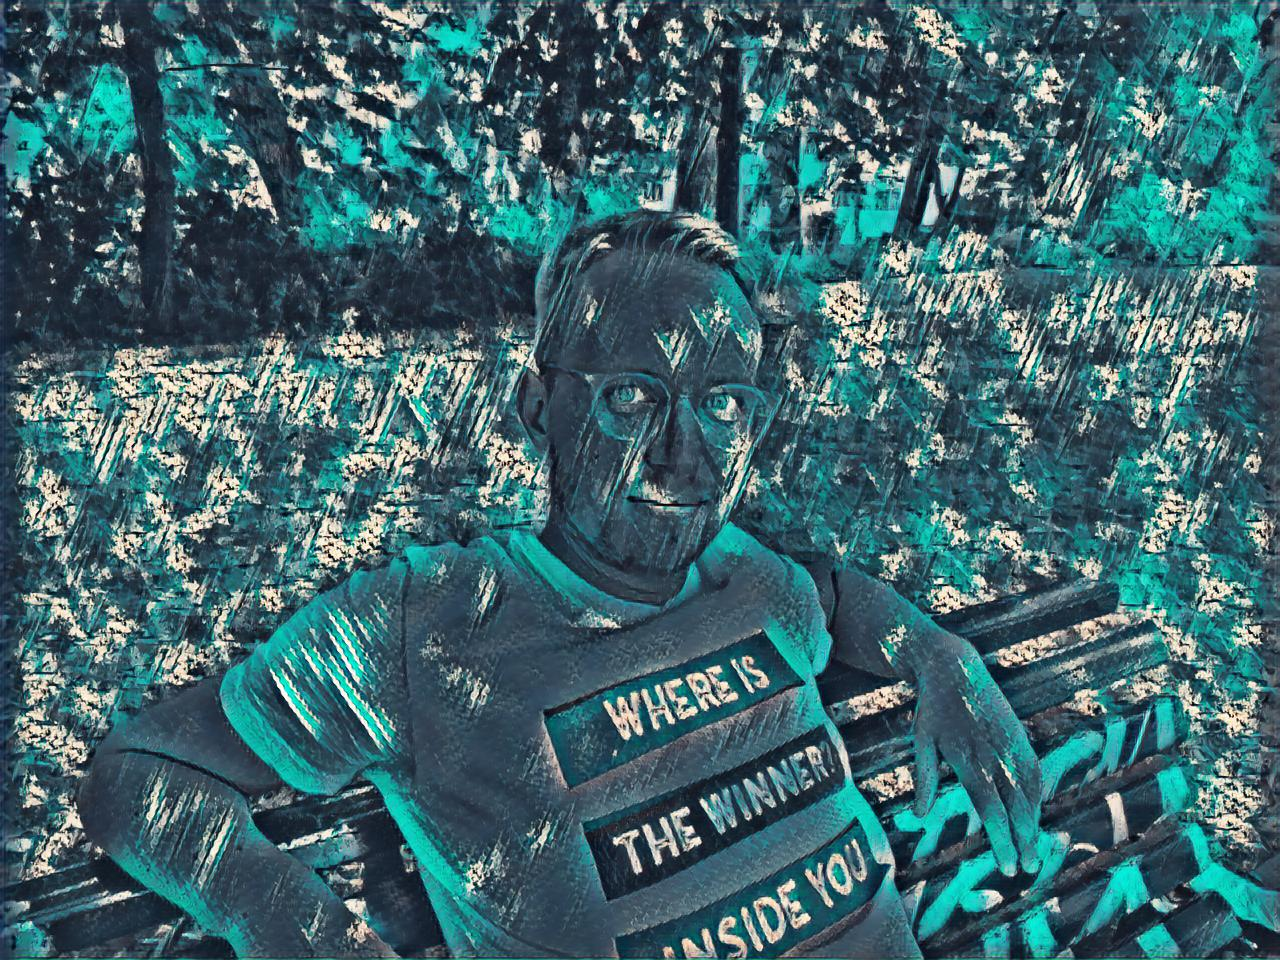
\includegraphics[width=\textwidth]{resources/content/experiments/ich-vgg16_teal_and_black_abstract_painting.jpg}
    \end{subfigure}
    \begin{subfigure}[h]{0.32\textwidth}
        \centering
        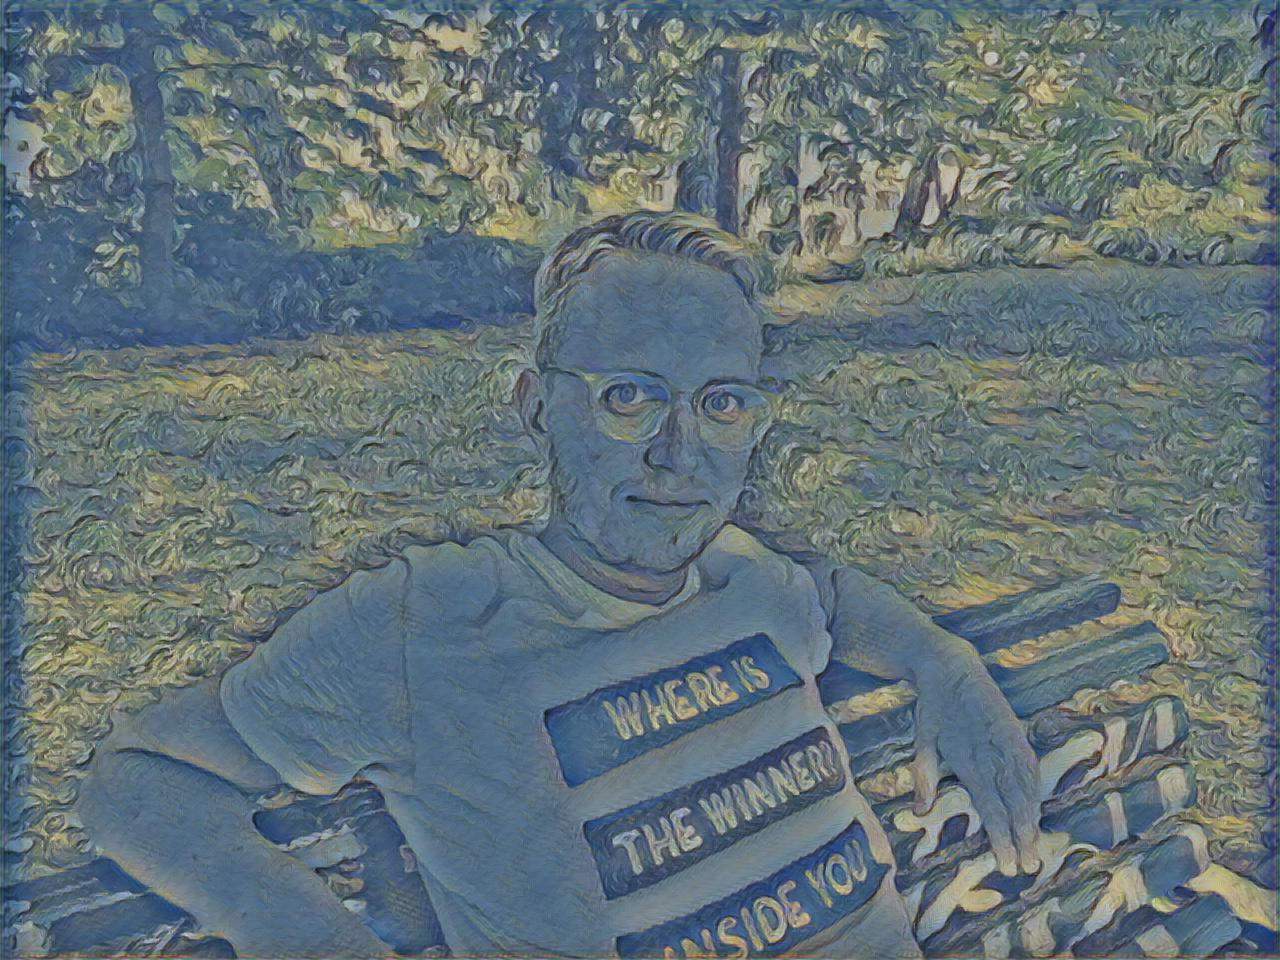
\includegraphics[width=\textwidth]{resources/content/experiments/ich-vgg16_the_olive_trees.jpg}
    \end{subfigure}

    \begin{subfigure}[h]{0.32\textwidth}
        \centering
        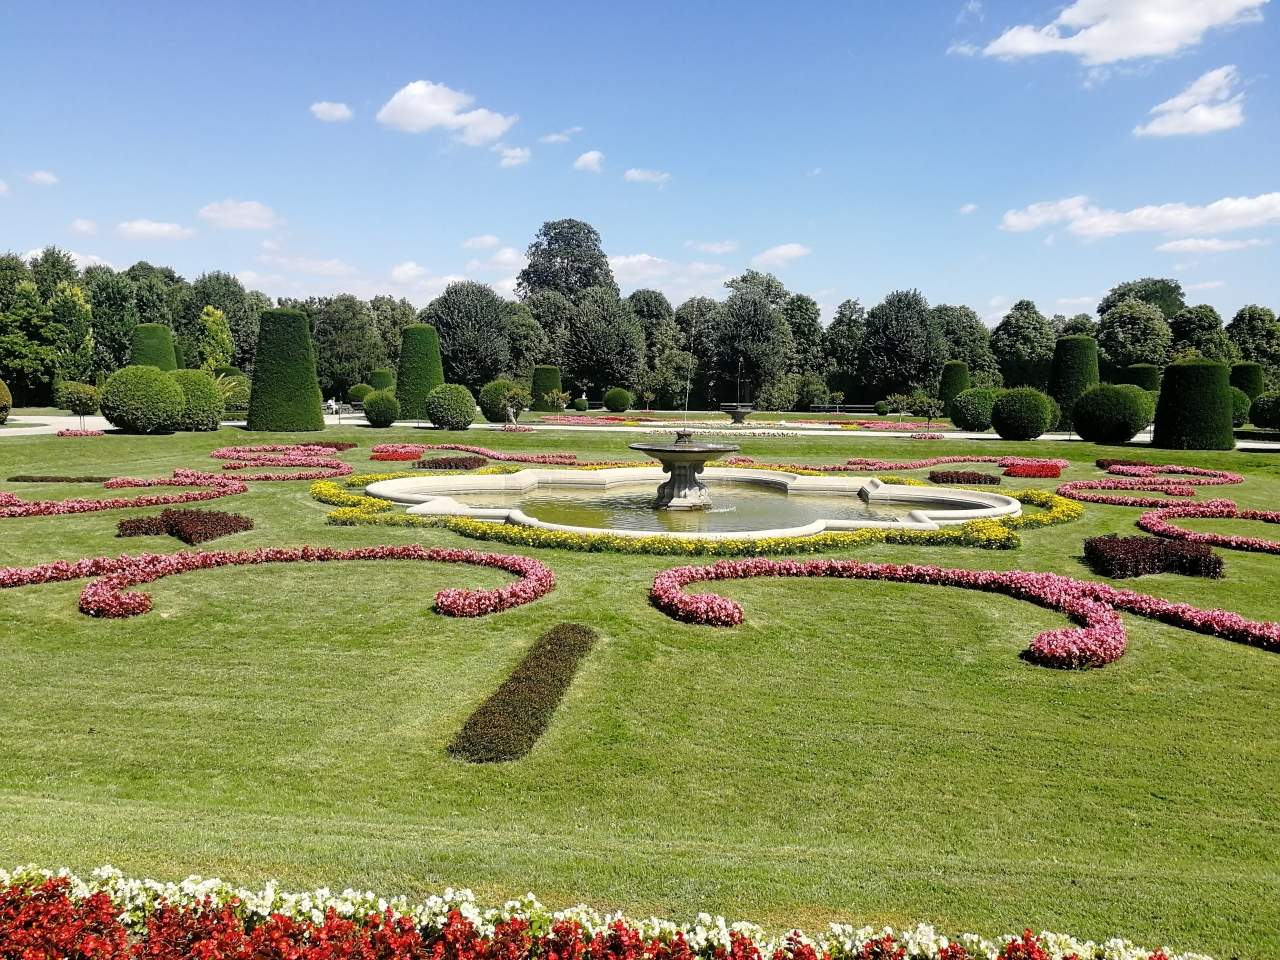
\includegraphics[width=\textwidth]{resources/content/content/garden.jpg}
    \end{subfigure}
    \begin{subfigure}[h]{0.32\textwidth}
        \centering
        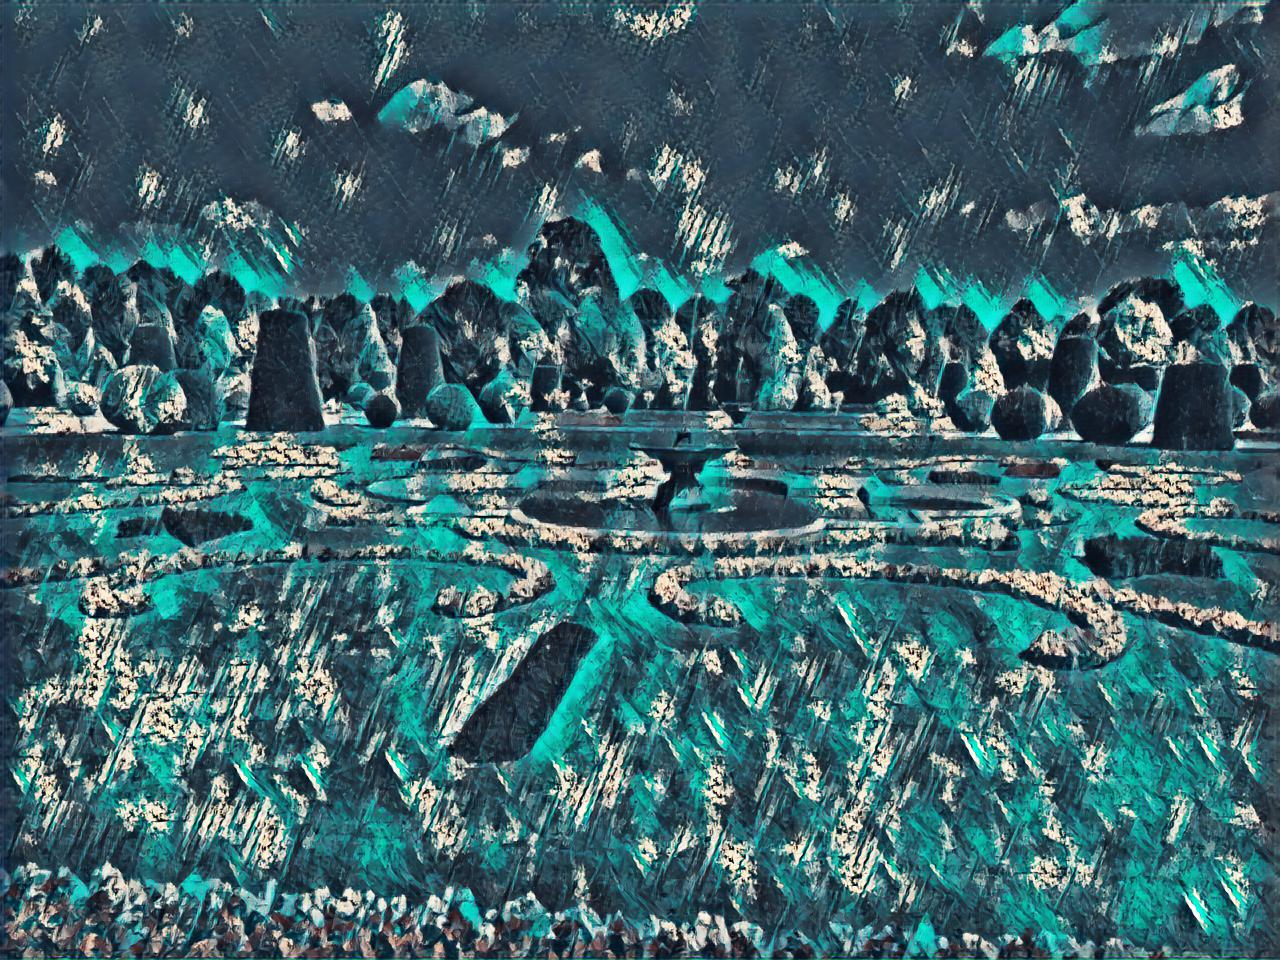
\includegraphics[width=\textwidth]{resources/content/experiments/garden-vgg16_teal_and_black_abstract_painting.jpg}
    \end{subfigure}
    \begin{subfigure}[h]{0.32\textwidth}
        \centering
        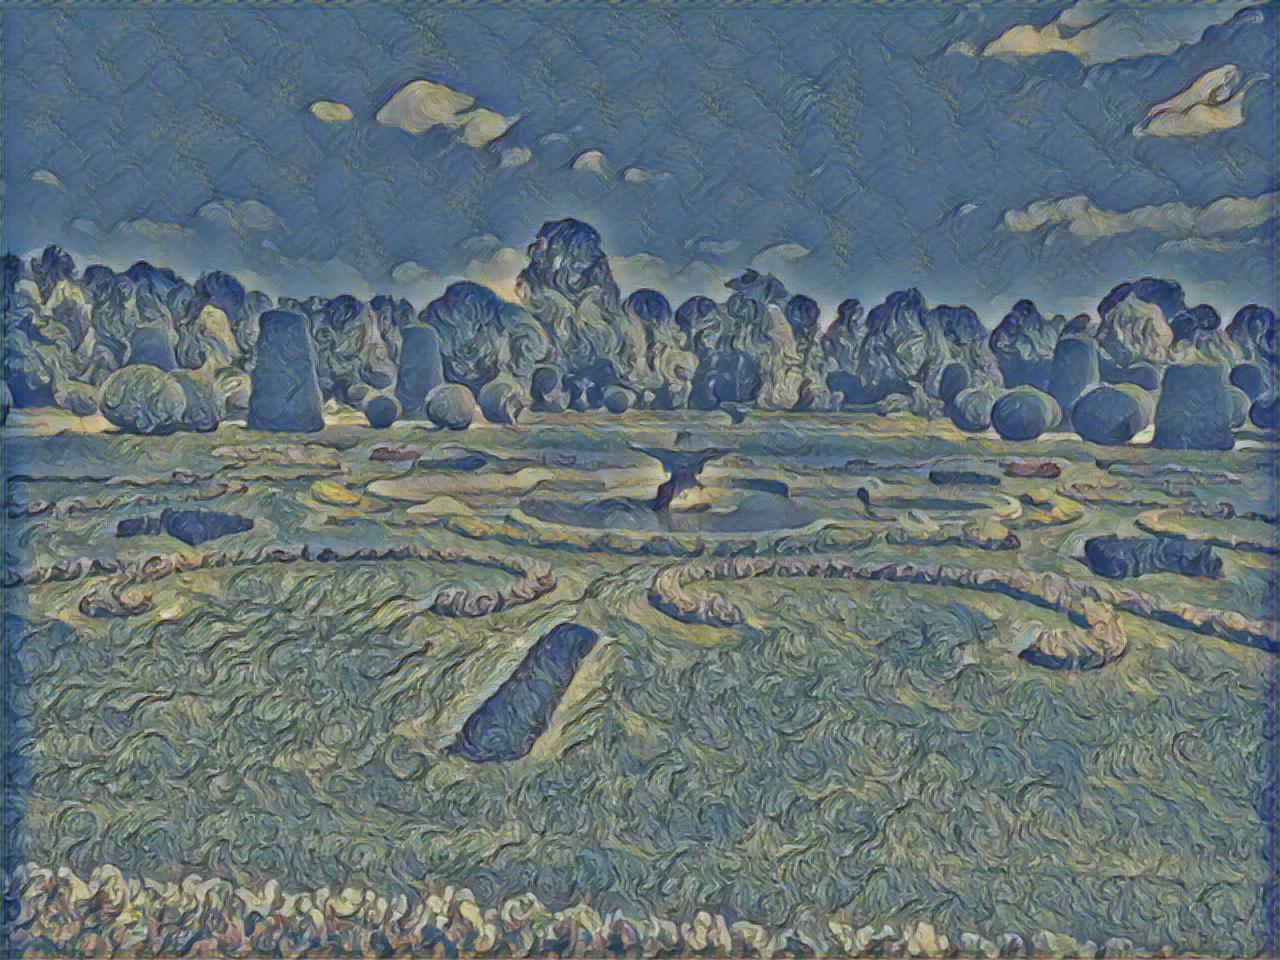
\includegraphics[width=\textwidth]{resources/content/experiments/garden-vgg16_the_olive_trees.jpg}
    \end{subfigure}

    \caption{Eigene Abbildungen kombiniert mit verschiedenen Stilen: \cite{teal_and_black_abstract_painting_img}, \cite{the_olive_trees_img}}
    \label{img:trained_models3}
\end{figure}